\documentclass{article}
\usepackage[a4paper, top=1in, bottom=1in, left=1in, right=1in]{geometry}
\usepackage[utf8]{inputenc}

\usepackage[english]{babel}
\usepackage{tikz-cd, lipsum, bm, dcolumn}
\usetikzlibrary{arrows}
\usepackage{amsmath, amssymb, amsthm, mathrsfs, mathtools, centernot, hyperref, fancyhdr, lastpage}


\renewcommand{\thispagestyle}[1]{}

\DeclareMathOperator{\Tr}{Tr}
\DeclareMathOperator{\Sym}{Sym}
\DeclareMathOperator{\Span}{span}
\DeclareMathOperator{\im}{Im}
\DeclareMathOperator{\Div}{div}
\DeclareMathOperator{\curl}{curl}
\DeclareMathOperator{\GL}{GL}
\DeclareMathOperator{\SL}{SL}
\DeclareMathOperator{\GA}{GA}
\DeclareMathOperator{\std}{std}
\DeclareMathOperator{\Cov}{Cov}
\DeclareMathOperator{\Var}{Var}
\DeclareMathOperator{\Corr}{Corr}
\DeclareMathOperator{\Int}{Int}
\DeclareMathOperator{\Id}{Id}
\DeclareMathOperator{\Lie}{Lie}
\DeclareMathOperator{\Hom}{Hom}
\DeclareMathOperator{\Alt}{Alt}
\DeclareMathOperator{\rank}{rank}
\DeclareMathOperator{\conv}{conv}
\DeclareMathOperator{\aff}{aff}
\DeclareMathOperator{\arccot}{arccot}


\newtheorem{theorem}{Theorem}[section]
\newtheorem{proposition}[theorem]{Proposition}
\newtheorem{lemma}[theorem]{Lemma}
\newtheorem{example}{Example}[section]
\newtheorem{corollary}{Corollary}[theorem]
\theoremstyle{remark}
\newtheorem*{remark}{Remark}
\theoremstyle{definition}
\newtheorem{definition}{Definition}[section]
\renewcommand{\qed}{\hfill$\blacksquare$}
\renewcommand{\footrulewidth}{0.4pt}% default is 0pt


\begin{document}
\pagestyle{fancy}

\lhead{Linear Algebra}
\chead{Muchang Bahng}
\rhead{\date{August 2021}}
\cfoot{\thepage / \pageref{LastPage}}

\title{Linear Algebra}
\author{Muchang Bahng}
\date{November 2022}

\maketitle

A multiple-year course in linear algebra at the advanced undergraduate and graduate level. The notes for this section can be a bit too abstract for someone learning linear algebra for the first time, so I suggest learning about groups, rings, and fields first. 

\section{Vector Spaces and Dual Spaces}
\begin{definition}[Vector Space]
A \textit{vector space} $V$ over a field $\mathbb{F}$ (usually $\mathbb{R}$ or $\mathbb{C}$) is a set of vectors that is algebraically closed under the operations: 
\begin{enumerate}
    \item $+: V \times V \longrightarrow V$
    \item $\times: \mathbb{F} \times V \longrightarrow V$
\end{enumerate}
It is also an additive abelian group, with additional axioms. That is, given $\lambda, \mu \in \mathbb{F}$ and $v, u \in V$, 
\begin{enumerate}
    \item $(\lambda + \mu) v = \lambda v + \mu v$
    \item $\lambda (v + u) = \lambda v + \lambda u$
    \item $(\lambda \mu) v = \lambda (\mu v) = \mu (\lambda v)$ 
\end{enumerate}
\end{definition} 

\begin{definition}
A \textit{vector} is an element of a vector space. 
\end{definition}

\begin{proposition}
There are no zero divisors of vector space $V$. That is, 
\[\lambda v = 0 \implies \lambda = 0 \text{ or } v = 0\]
\end{proposition}
\begin{proof}
$\lambda v = 0 \implies \lambda v + \lambda v = 0 + \lambda v \implies 2\lambda v = \lambda v \implies (2\lambda - \lambda ) v = 0$. But $\lambda \neq 0$, so $v$ must equal $0$. This leads to a contradiction. 
\end{proof}

We now introduce some classic interpretations of vectors. 

\begin{example}
$n$-tuples of elements of a field $\mathbb{F}$, that is, in the form
\[(a_1, a_2, ..., a_n)\]
are elements of a vector field, with vector addition and scalar multiplication defined component-wise. 
\end{example}

\begin{example}
The set of all arrows in space, with addition defined by the parallelogram rule and scalar multiplication defined as the stretching/compressing of the arrow from the origin, forms the vector space of arrows. 
\end{example}

We define some more vector spaces that are often used. 

\begin{example}
The set of all polynomials of degree strictly less than $n$ with coefficients in $\mathbb{F}$ defines a vector space over $\mathbb{F}$. 
\end{example}

\begin{definition}
A subset $Y$ of a linear space $X$ is called a \textit{subspace} if sums and scalar multiples of elements of $Y$ belong to $Y$. Note that $\{ 0 \}, X$ are subspaces of $X$. 
\end{definition}

\begin{definition}
Given vector spaces $U, V$ over the same field $\mathbb{F}$, a mapping $f: V \longrightarrow U$ that has properties 
\[ f(v_1 + v_2) = f(v_1) + f(v_2), \; \; f(c v) = c f(v), (c \in \mathbb{F})\]
is called a \textit{homomorphism}. The set of all homomorphisms from $V$ to $U$ is denoted Hom$(V, U)$. If $f$ is bijective, then $f$ is called an \textit{isomorphism}, and $U$ is said to be \textit{isomorphic} to $V$, denoted $U \simeq V$. Elements of Hom$(U,U)$, denoted End$(U)$, are called \textit{endomorphisms} of $U$, and an endomorphism of $U$ that is also an isomorphism is called an \textit{automorphism}. The set of all automorphisms of $U$ is denoted Aut$(U)$. 
\end{definition}

\subsection{Basis and Dimension}
\begin{definition}
A \textit{linear combination} of $j$ vectors $v_1, v_2, ..., v_j$ of a linear space is a vector of the form 
\begin{equation}
    c_1 v_1 + c_2 v_2 + c_3 v_3 + ... + c_j v_j, c_1, ..., c_j \in \mathbb{F}
\end{equation}
\end{definition}

\begin{definition}
The \textit{span} of a collection of vectors $v_1, v_2, ..., v_j \in V$ is the set
\[\Span \{ v_1, v_2, ..., v_j \} \equiv \{ c_1 v_1 + c_2 v_2 + c_3 v_3 + ... + c_j v_j\; | \; c_1, ..., c_j \in \mathbb{F}\} \]
That is, $\Span \{v_1, v_2, ..., v_j\}$ is the smallest subspace of $V$ that contains all $v_1, ..., v_j$. 
\end{definition}

It clearly follows that $v_1, ..., v_n$ span the whole space $V$ if every vector in $V$ can be expressed as a linear combination of the $v_i$'s. 

\begin{definition}
Vectors $v_1, ..., v_j$ are \textit{linearly independent} if 
\[ c_1 v_1 + c_2 v_2 + c_3 v_3 + ... + c_j v_j = 0 \implies c_1, ..., c_j = 0\]
They are \textit{linearly dependent} if there exists nonzero $c_1, ..., c_j$ such that the equality holds true, which is equivalent to saying that there is at least one vector $v_i, 1 \leq i \leq j,$ such that it can be represented as a linear combination of all the other vectors. 
\end{definition}

\begin{definition}
A set of linearly independent vectors $v_1, ..., v_n$ that span vector space $V$ is called a \textit{basis} of $V$. These vectors $v_i$ are called \textit{basis vectors}. Note that this basis is not unique; it is actually highly un-unique. 
\end{definition}

\begin{definition}
The basis $e_i$ of $\mathbb{F}^n$ are the vectors with every element equal to $0$ except for the $i$th element, which is equal to $1$. 
\end{definition}

\begin{proposition}
Every possible basis of a vector space $V$ has the same number of vectors.
\end{proposition}

\begin{proposition}
Any maximal linearly independent subset $\{ e_1, e_2, ..., e_k\}$ of a set $S$ is a basis of $\Span S$. 
\end{proposition}

\begin{definition}
The number of vectors in a basis of vector space $V$ is called the \textit{dimension} of $V$, denoted $\dim{V}$. 
\end{definition}

\begin{theorem}
Every $n$-dimensional vector space $V$ over $\mathbb{F}$ is isomorphic to $\mathbb{F}^n$, the set of $n$-tuples of elements in $\mathbb{F}$. 
\end{theorem}

\begin{corollary}
Vector spaces of the same field are isomorphic if and only if their dimensions are the same. 
\end{corollary}

\begin{example}
The field of complex numbers $\mathbb{C}$, regarded as a vector space over $\mathbb{R}$, has dimension $2$. The algebra of quaternions $\mathbb{H}$ has dimension $4$. 
\end{example}

\begin{definition}
A $(n - 1)$-dimensional subspace of an $n$-dimensional space is called a \textit{hyperplane}. 
\end{definition}

\begin{definition}
The sum of subspaces $U_1, U_2, ..., U_n \subset V$, denoted
\[U_1 + U_2 + U_3 + ... + U_n\]
is called the \textit{sum} of the subspaces $U_1, ..., U_n$. It is the set of all vectors that can be expressed as the sum of vectors in each of its respective space. That is, 
\[ \sum_{i=1}^n U_i \equiv \Big\{ \sum_{i = 1}^n u_i \;|\; u_i \in U_i\Big\}\]

\end{definition}

\begin{definition}[Direct Sum of Spaces]
Given subspaces $V_1, V_2, ..., V_n \subset V$ where the intersection between two $V_i$'s are pairwise disjoint, the \textit{direct sum} of the subspaces is the set of vectors that can be expressed uniquely as the sum of vectors in each of its respective spaces. That is, 
\[\bigoplus_{i=1}^n V_i \equiv \Big\{ \sum_{i=1}^n v_i \; | \; v_i \in V_i\Big\}\]
$V_1 \oplus V_2 \oplus ... \oplus V_n$ is also a vector space. 
\end{definition}

The crucial difference between the sum and the direct sum is that the direct sum requires the subspaces to be disjoint except for at the origin, which allows the expression of each vector in $V_1 \oplus ... \oplus V_n$ to be unique. It is also worth noting that the Cartesian product of vector spaces is merely just the set of tuples of vectors that are in each respective space and is \textit{not} a vector space (since addition and multiplication is not defined on that new set). If we define the operations component-wise, then 
\[ \prod_{i=1}^n V_i = \sum_{i=1}^n V_i\]

Note that we can also define the direct sum of spaces $U$ and $V$ by their basis. That is, given that the basis for $U$ is $\{e_i\}_{i=1}^n$ and the basis for $V$ is $\{f_j\}_{j=1}^n$, the basis for $U \oplus V$ is
\[\{(e_1, 0), (e_2, 0), ..., (e_n, 0), (0, f_1), ..., (0, f_m)\} \]

\begin{proposition}
\[\dim{\bigoplus_{i=1}^n V_i} = \sum_{i=1}^n \dim{V_i}\]
\end{proposition}
\begin{proof}
This follows from the basis construction of the direct sum of $V_i$'s. 
\end{proof}

\begin{definition}[Congruence Relations on Vector Spaces]
Given vector space $X$ and subspace $Y$ we say that two vectors $x_1$ and $x_2$ are \textit{congruent modulo $Y$}, denoted 
\[ x_1 \equiv x_2 \pmod{Y}\]
if $x_2 - x_1 \in Y$. This congruence is a \textit{relation}, meaning that it is symmetric, reflective, and transitive (elaborated in the abstract algebra chapter). The \textit{congruence classes} $\{ y\}$ is the set of all vectors that are congruent modulo $Y$ to $y$. 
\end{definition}

\begin{definition}[Quotient Vector Space]
The \textit{quotient space} modulo $Y$, denoted $ X / Y$, is the set of all congruence classes modulo $Y$. We can define addition and scalar multiplication on this set as such 
\[ \{ x\} + \{ y\} = \{ x + y\}\]
\end{definition}

\begin{proposition}
Given vector space $X$, $Y$ a subspace of $X$. Then, 
\[ X \simeq Y \oplus \frac{X}{Y}\]
\end{proposition}

Vector spaces over one field can be interpreted as a vector space over another field. This is most common when interpreting complex vector spaces as real ones. For example, given a complex vector space $Z$ with basis $\{z_1, z_2, ..., z_n\}$, every vector can be expressed as
\[z = \sum_{j=1}^n c_j z_j, \; c_j \in \mathbb{C}\]
We can set $c_j = a_j + b_j i$ uniquely, with $a, b \in \mathbb{R}$, and rewrite
\[z = \sum_{j=1}^n a_j z_j + b_j (i z_j)\]
$\implies \{ z_j\} \cup \{ i z_j\}$ forms a basis of $Z$ as a \textit{real vector space}. 

\subsection{Dual Spaces}
\begin{definition}
A \textit{linear map} is a homomorphism between vector spaces. That is, a linear map $f: X \longrightarrow Y$ has the properties 
\begin{align*}
    & \forall u, v \in X \; f(u + v) = f(u) + f(v) \\
    & \forall u \in X, c \in \mathbb{F} \; f(c u) = c f(u) 
\end{align*}
\end{definition}

\begin{definition}[Dual Space]
Given a vector space $V$ over $\mathbb{F}$, the \textit{dual vector space} $V^*$ is the set of all linear maps that, given a vector in $V$, outputs a scalar in $\mathbb{F}$. That is, 
\[ V^* \equiv \{ l \text{ linear} \; | \; l: V \longrightarrow \mathbb{F}\}\]
or equivalently, 
\[V^* \equiv \text{Hom}(V, \mathbb{F})\]
The addition and scalar multiplication of $V^*$ is defined pointwise. That is, given $l, m \in V^*$, 
\[(l + m) (x) = l(x) + m(x), \; (c l)(x) = c l(x)\]
\end{definition}

\begin{theorem}
\[ \dim{V} = n \implies \dim{V^*} = n\]
\end{theorem}

While we initially view elements of $V$ as "things" and elements of $V^*$ as linear functions, this thought is actually erroneous. Given $l \in V^*$, we see that 
\[l: V \longrightarrow \mathbb{F}\]
But since both $V$ and $V^*$ are vector spaces, we can also see that given $x \in V$, $x$ is also a linear function 
\[x: V^* \longrightarrow \mathbb{F}, \text{ where } x(l) \equiv l(x)\]
But this means that $x$ is an element of $V^{**}$ the dual of $V$! This statement is elaborated with the following theorem. 

\begin{theorem}[Canonical Isomorphisms of Double Duals]
$V^{**}$ is \textit{naturally, or canonically, isomorphic} to vector space $V$. However, $V$ is not naturally isomorphic to $V^*$. 
\end{theorem}

\begin{proof}
What we mean by natural is that we do not need to select a basis in either vector space to define the isomorphism. We fix a vector $l \in V^*$, and given $x \in V, \phi \in V^{**}$, we define
\[ \phi(l) \equiv l(x) \]
This defines a one-to-one correspondence between $V$ and $V^{**}$. On the contrary, there is no way to define an isomorphism between $V$ and $V^*$ without further structure on $V$. 
\end{proof}

It is important to be aware of this \textit{duality} between elements $x \in V$ and $l \in V^*$, and thus we should interpret $x \in V$ as a linear function of $V^*$ and $l \in V^*$ as a linear function of $V$.

\begin{definition}
Given a basis $\{ e_1, e_2, ..., e_n\}$ of $V$, the \textit{dual basis} $\{f_1, f_2, ..., f_n\}$ of $V^*$ has vectors satisfying 
\[ f_j (e_i) = \delta_{i j} = 
\begin{cases}
0 & i \neq j \\
1 & i = j
\end{cases}\]
where $\delta_{i j}$ is called the \textit{Kronecker delta function}. 
\end{definition}

\begin{definition}[Annihilator]
Let $Y$ be a subspace of $X$. Then the set of functions in $X^*$ that vanish on $Y$, that is, satisfy
\[l(y) = 0 \text{ for all } y \in Y\]
is called the \textit{annihilator} of $Y$, denoted $Y^0$. If $Y = X$, then it is easy to see that $Y^0$ is trivial. 
\end{definition}

\begin{theorem} Given subspace $Y$ of $X$ 
\[ Y^0 \simeq (X / Y)^*\]
\end{theorem}

\begin{proof}
The isomorphism is defined as such. Given $l \in Y^0$, we define $L \in (Y/X)^*$ as 
\[L\{x\} \equiv l(x)\]
\end{proof}

\begin{corollary}
\[\dim Y^0 + \dim Y = \dim X\]
\end{corollary}

\begin{corollary}
\[Y^{0 0} = Y\]
\end{corollary}

\begin{theorem}
Let $l$ be an interval on $\mathbb{R}$ containing $t_1, t_2, ..., t_n$ $n$ distinct points. Then, given any polynomial $p$ with degree $< n$, there exist $n$ real numbers $c_1, c_2, ..., c_n$ such that
\[ \int_l p(t) d t = c_1 p(t_1) + c_2 p(t_2) + ... + c_n p(t_n)\]
called the \textit{quadrature formula} suffices. That is, the integral of any polynomial over $l$ can be expressed as a linear combination of the polynomials evaluated at $n$ distinct points in $l$. 
\end{theorem}

\begin{proof}
The space of all polynomials with degree $< n$ is an $n$-dimensional vector space, denote it $V$. We define the basis of the dual space $V^*$ as 
\[\phi_i (p) \equiv p(t_i), \; i = 1, 2, ..., n\]
with addition and scalar multiplication defined
\begin{align*}
    & (\phi + \gamma) (p) \equiv \phi(p) + \gamma(p) \\
    & (c \phi) (p) \equiv c \phi (p) 
\end{align*}
We can see that the $\phi$'s are indeed linear since, given $p, q \in \mathbb{R}[t]$
\begin{align*}
    & \phi_i (p + q) = (p + q) (t_i) = p(t_i) + q(t_i) = \phi_i (p) + \phi_i (q) \\
    & \phi_i (c p) = (c p) (t_i) = c p(t_i) = c \phi_i (p)
\end{align*}
We claim that all the $phi_i$'s are linearly independent. Assume that \[\sum_{i=1}^n c_i \phi_i (p) = \sum_{i=1}^n c_i p(t_i) = 0\]
Since the $\phi$'s must be linearly independent for every polynomial $p$, set it equal to
\[q_k (t) \equiv \prod_{j \neq k} (t - t_j), \; k = 1, 2, ..., n\]
$p = q_k$ must imply that all $\phi_i (p) = 0$ for all $i \neq k$, which implies that $c_k = 0$ in the linear combination. Repeating this for $k = 1, 2, ..., n$ results in all $c_i = 0$, implying that the $\phi_i$'s form a basis of $V^*$. Clearly, the function of definite integration over $l$ is a linear mapping from $V \longrightarrow \mathbb{R}$, meaning that it is in $V^*$. Therefore, it can be expressed as a linear combination of $\phi_i$'s. 
\end{proof}

\section{Linear Maps}
Remember that a linear transformation is just a homomorphism between vector spaces. That is, given linear transformation $T: U \longrightarrow V$, 
\[T \in \text{Hom}(U,V)\]
We can visualize all linear transformations as "transforming" the axes as shown below. 
\begin{center}
    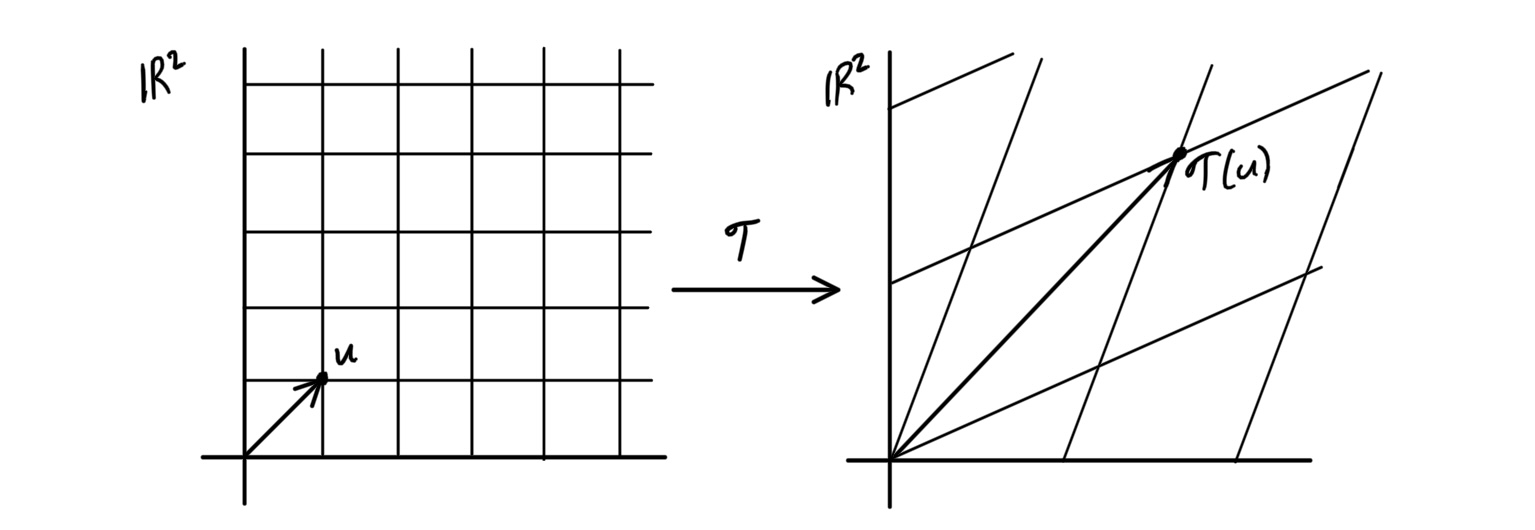
\includegraphics[scale=0.25]{Images/Linear_Map.PNG}
\end{center}

\begin{definition}[Image]
The \textit{image or range} of $T: U \longrightarrow V$ is the image of $U$ under $T$, denoted Im$T$. 
\[\im{T} \equiv \{ T(u) \; | \; u \in U\} \subset V\]
The \textit{kernel or nullspace} of $T$ is the subset of $U$ that is mapped onto $0$, denoted ker$T$. 
\[\text{ker}\,T \equiv \{ u \in U \; | \; T(u) = 0\} \]
\end{definition}

\begin{example}
Let $U_1$ be a subspace of $U$ and given the quotient map
\[ \pi: U \longrightarrow U / U_1\]
Then, 
\[\text{ker}\,\pi = U_1, \; \im{\pi} = U / U_1\]
Note that a quotient map is always surjective. 
\end{example}

\begin{theorem}[Rank Nullity Theorem]
Let $T: U \longrightarrow V$ be linear. Then, 
\[ \dim \ker T + \dim \im T = \dim U\]
This theorem is quite intuitive, if we visualize the map. We just have to realize that given a linear transformation mapping from a $n$-dimensional $V$ to a $m$-dimensional $U$, every vector in $V$ will either get mapped to $0 \in U$ or will get mapped to a nonzero vector in $U$. 
\begin{center}
    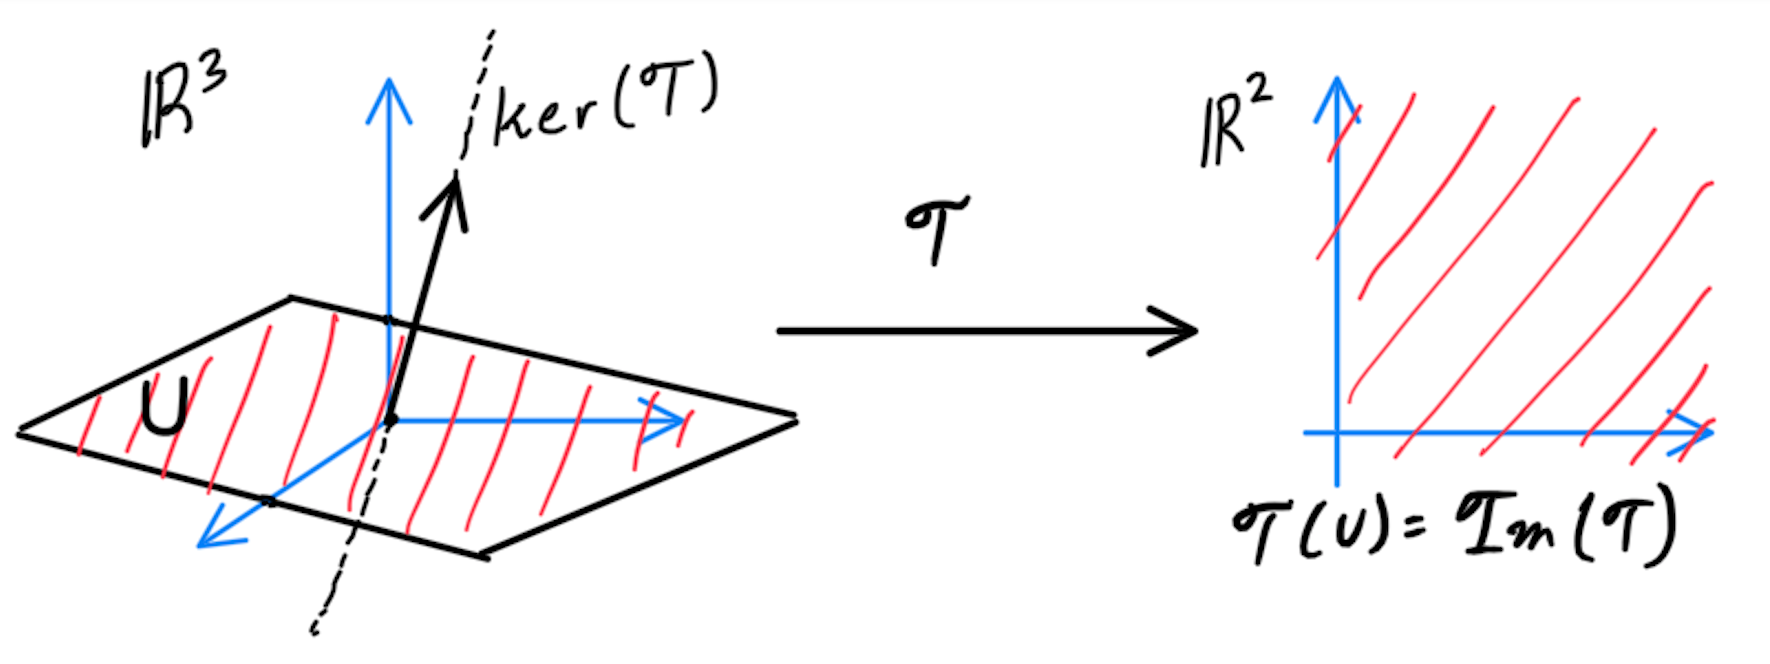
\includegraphics[scale=0.4]{Images/Rank_Nullity.PNG}
\end{center}
\end{theorem}

\begin{proposition}
Hom$(U, V)$ is the vector space of linear mappings, with addition and scalar multiplication defined
\begin{align*}
    & (S + T) (x) \equiv S(x) + T(x) \\
    & (c T) (x) \equiv c T(x)
\end{align*}
\end{proposition}

\begin{definition}
The \textit{composition} of linear functions, denoted with $\circ$, is defined
\[ (S \circ T) (x) \equiv S\big( T(x)\big) \]
Given $T \in $ Hom$(U, V)$ and $S \in $ Hom$(V, W)$, then $S \circ T \in $ Hom$(U, W)$. For simplicity, we also denote the composition as 
\[ S \circ T \equiv S T\]
\end{definition}

\begin{proposition}
Composition is (right and left) distributive with respect to the addition of linear maps. That is, 
\begin{align*}
    & (R + S) \circ T = R \circ T + S \circ T \\
    & T \circ (R + S) = T \circ R + T \circ S 
\end{align*}
\end{proposition}

\begin{definition}
An \textit{algebra} $A$ is a vector space with the additional operation of vector multiplication. That is, $A$ is closed under 
\[\circ: A \times A \longrightarrow A\] 
An algebra is \textit{associative} if multiplication is associative. That is, given $R, S, T \in A$
\[ R \circ (S \circ T) = (R \circ S) \circ T \]
Note that multiplication is not necessarily commutative. 
\end{definition}

\begin{proposition}
End$(V)$ is an associative, noncommutative algebra. 
\end{proposition}

\begin{example}
A rotation around any axis or a flip across any hyperplane is an element of End$(\mathbb{R}^n)$. 
\end{example}

\begin{definition}
A \textit{projection mapping} is a linear mapping $P$ where 
\[ P = P^2\]
\end{definition}

\begin{example}
Let $P$ be an orthogonal projection mapping onto a subspace $Y$ of $X$. $\im P = Y$, and $\ker P = Y^\perp$ or the span of vectors in $X$ that are "orthogonal" to $Y$. Note that we haven't actually endowed a structure onto $X$ to even define orthogonality yet, so this definition is purely visual and not mathematically rigorous. 
\end{example}

\begin{example}
Reflections, projections, shears, and rotations are all linear maps. Differentiation and integration are also examples of linear mappings. 
\end{example}

\begin{remark}
Linear maps over vector spaces over different fields are generally not well defined since the definition of homomorphisms do not cover the fields in which vector spaces are associated with. 
\end{remark}

\begin{theorem}
Given $A: V \longrightarrow U$ a linear mapping between vector spaces and $b \in U$, all solutions to the equation $Ax = b$ is in $a + \ker A$, that is, of the form 
\[ x = a + y, \; y \in \ker A\]
where $x = a$ is one solution. 
\end{theorem}

\begin{corollary}
A linear map $A$ is injective if and only if $\ker A = 0$.
\end{corollary}

\begin{definition}
The \textit{rank} of a linear map $A$ is the dimension of its image. 
\end{definition}

\subsection{Factorization of Linear Maps}
\begin{definition}
Let $\varphi: U \longrightarrow V$ be a linear mapping and let $U_1 \subset U, V_1 \subset V$ be subspaces. Such that \[\varphi u \in V \text{ for all } u \in U\]
Then, the linear mapping 
\[\varphi_1: U_1 \longrightarrow V_1, \; \varphi_1 u = \varphi_u, u \in U_1\]
is called the \textit{restriction} of $\varphi$ to $U_1, V_1$. It suffices the identity
\[\varphi \circ i_U = i_V \circ \varphi_1\]
where $i_U: U_1 \longrightarrow U, i_V: V_1 \longrightarrow V$ are canonical injections. Equivalently, we say that the diagram below is \textit{commutative}. 
\[
  \begin{tikzcd}
    U \arrow{r}{\varphi} & V \\
    U_1 \arrow{u}{i_U} \arrow{r}{\varphi_1} & V_1 \arrow{u}{i_V}
  \end{tikzcd}
\]
We can also define 
\[\varphi_1 \equiv i_v^{-1} \varphi i_U\]
\end{definition}

The construction of the restriction is an enormously helpful tool for many proofs and very useful for factoring linear mappings. 

\begin{definition}
Given $\varphi: U \longrightarrow V$ with quotient maps 
\[\pi_U: U \longrightarrow U / U_1, \; \pi_V: V \longrightarrow V / V_1 \]
the \textit{induced mapping of the quotient spaces} is the unique mapping $\bar{\varphi}: U/U_1 \longrightarrow V / V_1$ such that 
\[\bar{\varphi} \circ \pi_U = \pi_V \circ \varphi\]
or equivalently, the following diagram commutes. 
\[\begin{tikzcd}
    U \arrow{r}{\varphi} \arrow{d}{\pi_U} & V \arrow{d}{\pi_V}\\
    U / U_1 \arrow{r}{\bar{\varphi}} & F / F_1
\end{tikzcd}\]
\end{definition} 

\begin{theorem}
Every linear mapping can be written as the composition of a surjective mapping followed by an injective mapping. That is, every $A$ can be factored into 
\[A = A_{inj} \circ A_{surj}\]
\end{theorem}
\begin{proof}
We can induce a quotient mapping to construct a factoring of a linear mapping. We can define the unique mapping 
\[\bar{\varphi}: U / \ker{U} \longrightarrow F\]
such that, $\varphi = \bar{\varphi} \circ \pi_U$, or that 
\[\begin{tikzcd}
     U \arrow{r}{\varphi} \arrow{d}{\pi_U} & V \\
     U / \ker{\varphi} \arrow{ru}{\bar{\varphi}}
\end{tikzcd} \]
commutes. Clearly, $\bar{\varphi}$ is injective since if it were not, $\bar{\varphi} \pi_U x = 0 \implies \varphi x = 0 \implies x \in \ker{\varphi} \implies \pi_U x = 0$. This also means that the restriction of $\bar{\varphi}$ to $U / \ker{\varphi}$
\[\bar{\bar{\varphi}}: U / \ker{\varphi} \longrightarrow \im{\varphi}\]
is a linear isomorphism. Thus, for any $\varphi$, it can be written as $\bar{\varphi} \circ \pi_U$, with $\bar{\varphi}$ injective and $\pi_U$ surjective. 
\end{proof}

\begin{proposition}
Given $E_1, E_2$ subspaces of $E$. Then, 
\[\frac{E_1}{E_1 \cap E_2} \simeq \frac{E_1 + E_2}{E_2}\]
In fact, they are naturally isomorphic. 
\end{proposition}
\begin{proof}
$E_1 + E_2$ can be decomposed to $E_1^\prime \oplus (E_1 \cap E_2) \oplus E_2^\prime$, where $E_1^\prime$ consists of the subspace of vectors $x$ that can only be expressed as $x = x_1, x_1 \in E_1$ and $E_2^\prime$ are vectors that can only be expressed as $x = x_2, x_2 \in E_2$. Define the projection mapping
\[\text{proj}: E_1 + E_2 \longrightarrow E_1^\prime\]
Since $E_1 = E_1^\prime \oplus (E_1 \cap E_2)$, we can define the natural isomorphism 
\[\kappa: E_1^\prime \longrightarrow \frac{E_1}{E_1 \cap E_2}, \; \kappa{x} = \{x\}\]
We now define the mapping $\varphi: E_1^\prime \longrightarrow (E_1 + E_2) / E_2$ such that
\[\pi = \varphi \text{proj}\]
given by the diagram 
\[\begin{tikzcd} 
    E_1 + E_2 \arrow{d}{proj} \arrow{r}{\pi} & \frac{E_1 + E_2}{E_2} \\
    E_1^\prime \arrow{ru}{\varphi} \arrow{r}{\kappa} & \frac{E_1}{E_1 \cap E_2}
\end{tikzcd}\]
Such a $\varphi$ exists because proj is surjective and can thus be inverted. We now claim that $\varphi$ is an isomorphism. $\ker{\text{proj}} = \ker{\pi} = E_2 \implies \kappa$ is injective. Given $x = x_1 + y + x_2 \in E_1 + E_2$ such that $x_1 \in E_1^\prime, y \in E_1 \cap E_2, x_2 \in E_2^\prime$, 
\[\pi(x) = \pi(x_1 + y + x_2) = \pi(x_1) = \varphi \text{proj} (x_1) = \varphi (x_1)\]
meaning that for every vector $v \in (E_1 + E_2) / E_2$, it can be expressed as $v = \pi (x) = \varphi (x_1)$, meaning that there exists a $x_1 \in E_1^\prime$ mapping to $v$ under $\varphi \iff \varphi$ is surjective. So, $\varphi$ is an isomorphism $\implies \varphi \kappa^{-1}$ is an isomorphism.  
\end{proof}

\begin{corollary}
In the special case when $E_1 \oplus E_2 = E$, then the proposition states that 
\[E_1 \simeq \frac{E}{E_2}\]
\end{corollary}

Let $f_1, f_2, ..., f_n$ be any $n$ linear functionals of $U$. Define the subspace $F \subset E$ as 
\[ F \equiv \bigcap_{i=1}^n \ker{f_i}\]
and define linear map 
\[\phi: U \longrightarrow \mathbb{F}^n, \;\phi(x) \equiv (f_1(x), f_2(x), ..., f_n(x))\]
$\implies \ker{\phi} = F$. So, $\phi: U \longrightarrow \mathbb{F}^n$ defines the isomorphism 
\[\bar{\phi}: U / F \longrightarrow \im{\phi}\]

\begin{proposition}
Given linear mappings $\phi: E \longrightarrow F$, $\psi: E \longrightarrow G$ such that
\[\ker{\phi} \subseteq \ker{\psi}\]
Then there exists a map $\kappa$ such that 
\[ \psi = \kappa \phi\]
or equivalently, such that the diagram below commutes. 
\[\begin{tikzcd} 
    E \arrow{r}{\phi} \arrow{d}{\psi} & F \arrow{dl}{\kappa} \\
    G 
\end{tikzcd}\]
\end{proposition}

Now, we introduce the concept of exact sequences which is useful in the factoring of linear maps. Note that exact sequences are used in group theory to factor transformation groups. 

\begin{definition}
A sequence of linear mappings 
\[F \xrightarrow{\varphi} E \xrightarrow{\psi} G\]
is \textit{exact at E} if
\[ \im{\varphi} = \ker{\psi}\]
\end{definition}

Notice that if we have an exact sequence 
\[0 \xrightarrow{\varphi} E \xrightarrow{\psi} G\]
then, $0 = \im{\varphi} = \ker{\psi} \implies \psi$ is injective. If we have exact sequence 
\[F \xrightarrow{\varphi} E \xrightarrow{\psi} 0\]
then, $\im{\varphi} = \ker{\psi} = E \implies \varphi$ is surjective. 

\begin{definition}
A \textit{short exact sequence} is a sequence of the form
\[0 \xrightarrow{} F \xrightarrow{\varphi} E \xrightarrow{\psi} G \xrightarrow{} 0\]
such that it is exact at $F, E$, and $G$. It is clear that the first and last maps are the zero maps. With this definition, we can easily prove that

i) $\varphi$ is injective

ii) $\psi$ is surjective

iii) $E / \im{F} \simeq G$
\end{definition}

\begin{example}
The sequence 
\[0 \xrightarrow{} E_1 \xrightarrow{i} E \xrightarrow{\pi} E / E_1 \xrightarrow{} 0\]
is exact, where $i$ denotes the canonical injection and $\pi$ the canonical projection. This example is the only example of an exact sequence between vector spaces up to isomorphism. 
\end{example}

\begin{definition}
A commutative diagram of the form
\[\begin{tikzcd}
    0 \arrow{r} & F_1 \arrow{d}{\alpha} \arrow{r}{\varphi_1} & E_1 \arrow{d}{\beta} \arrow{r}{\psi_1} & G_1 \arrow{d}{\gamma} \arrow{r} & 0 \\
    0 \arrow{r} & F_2 \arrow{r}{\varphi_2} & E_2 \arrow{r}{\psi_2} & G_2 \arrow{r} & 0 
\end{tikzcd}\]
where both horizontal sequences are short exact sequences and $\alpha, \beta, \gamma$ are homomorphisms between linear spaces is a \textit{homomorphism of exact sequences}. If $\alpha, \beta, \gamma$ are linear isomorphisms, then this is an \textit{isomorphism of exact sequences}. 
\end{definition}

\begin{proposition}
A short exact sequence of vector spaces
\[0 \xrightarrow{} F \xrightarrow{\varphi} E \xrightarrow{\psi} G \xrightarrow{} 0\]
is split if it essentially presents $E$ as the direct sum of groups $F$ and $G$. That is, there exists an isomorphism of exact sequences.
\[\begin{tikzcd}
    0 \arrow{r} & F \arrow{d}{\alpha} \arrow{r}{\varphi_1} & E \arrow{d}{\beta} \arrow{r}{\psi_1} & G \arrow{d}{\gamma} \arrow{r} & 0 \\
    0 \arrow{r} & F \arrow{r}{\varphi_2} & F \oplus G \arrow{r}{\psi_2} & G \arrow{r} & 0 
\end{tikzcd}\]
or equivalently, there exists an isomorphism between $E$ and $F \oplus G$. 
\end{proposition}

\begin{definition}
Given a short exact sequence
\[0 \xrightarrow{} F \xrightarrow{\varphi} E \xrightarrow{\psi} G \xrightarrow{} 0\]
if there exists a map $\kappa: G \longrightarrow E$, such that $ \psi \circ \kappa = I$, then the sequence is said to be a \textit{split short exact sequence}, written
\[0 \xrightarrow{} F \xrightarrow{\varphi} E \xleftrightarrow{\psi, \kappa} G \xrightarrow{} 0\]
\end{definition}

\begin{proposition}
Every short exact sequence can be split. 
\end{proposition}
\begin{proof}
It will be proved later that $\psi$ is surjective $\implies$ $\psi$ is left invertible. 
\end{proof}

\begin{definition}
Given $\varphi: E \longrightarrow E$, a subspace $E_1 \subset E$ is called \textit{stable} 
\[x \in E_1 \implies \varphi x \in E_1\]
That is, the restriction of $\varphi$ to $E_1$, denoted
\[\varphi: E_1 \longrightarrow E_1\]
is well-defined. Clearly, $\im{\varphi}$ and $\ker{\varphi}$ is stable, and the induced map 
\[\bar{\varphi}: E / E_1 \longrightarrow E / E_1\]
is a linear endomorphism of $E / E_1$. 
\end{definition}

We end this subsection by defining the induced linear map from the direct sum of spaces. 
\begin{definition}
Given linear maps $A_i \in$ End$(V_i)$ for $i = 1, 2, ..., n$, the induced linear map
\[\bigoplus_{i =1}^n A_i: \bigoplus_{i=1}^n V_i \longrightarrow \bigoplus_{i=1}^n V_i\]
is defined
\[(\bigoplus_{i=1}^n A_i)(\bigoplus_{i=1}^n x_i) \equiv \bigoplus_{i=1}^n A_i x_i\]
\end{definition}

\subsection{Invertibility and Transpose}
We now introduce the concepts of left and right invertibility of linear mappings. 

\begin{theorem}
A linear mapping $T: U \longrightarrow V$, with $\dim{U} = n, \dim{V} = m$, is \textit{left-invertible}. That is, there exists linear $S$ such that 
\[S T = I\]
if and only if $T$ is injective $\iff$ rank$(T) = n$. Linear $T$ is \textit{right-invertible}, that is, there exists linear $S$ such that 
\[T S = I\]
if and only if $T$ is surjective $\iff$ rank$(T) = m$. 
\end{theorem}
\begin{proof}
We will only prove the case for left-invertibility. Right invertibility follows analogously. \\
$(\leftarrow)$ $T$ is injective $\implies$ rank$(T) = \dim{U} = \dim{\im{T}}$. Let $(\im{T})^\prime$ exist such that 
\[\im{T} \oplus (\im{T})^\prime = V\]
We define the isomorphism 
\[\Tilde{T}: V \longrightarrow \im{T}\]
and then define $S$. Given that $v = w + w^\prime \in V$, with $w \in \im{T}, w^\prime \in (\im{T})^\prime$, 
\[S : V \longrightarrow U, \; S(v) \equiv \Tilde{T}^{-1} (v)\]
$\implies S T (u) = \Tilde{T}^{-1} T (u) = u \iff S T = I$. \\
$(\rightarrow)$ We prove the contrapositive. $T$ is not injective $\implies \dim{\ker{T}} > 0 \implies $ there exists 2 linearly independent vectors $x, y \in U$ such that
\[T x = T y\]
Assume that a left inverse $S$ exists. Then 
\[x = S T x = S T y = y \implies x = y\]
leading to a contradiction $\implies$ the left-inverse does not exist. 
\end{proof}

\begin{definition}
The inverse of a linear map $A$, denoted $A^{-1}$ is a unique linear map satisfying 
\[ A A^{-1} = A^{-1} A = I\]
where $I$ is the identity map. 
\end{definition}

\begin{corollary}
A linear map is invertible if and only if it is an isomorphism. 
\end{corollary}

We finally end this section by defining the transpose of a linear mapping. 

\begin{definition}
Given a linear mapping $A: U \longrightarrow V$, let there exist a certain $\varphi \in V^*$. Then, there exists a corresponding $l \in U^*$ such that 
\[ l \equiv \varphi A \]
This mapping $A^T: V^* \longrightarrow U^*$ that assigns every $\varphi$ to a corresponding $l$ is called the \textit{transpose} of $A$. Note that the transpose is canonically formed when defining any linear map. We do not need any additional structure on $U$ or $V$ to define $A^T$.
\[
  \begin{tikzcd}
    U \arrow{r}{A} \arrow[swap]{dr}{l = \varphi A} & V \arrow{d}{\varphi} \\
    & \mathbb{F}
  \end{tikzcd}
\]
\end{definition}

It is worth mentioning that $A^T$ maps every element in the annihilator $V^0$ to an element in $U^0$, but not necessarily the other way around. 

\begin{theorem}
\[ (\im A)^0 = \ker A^T \text{ or equivalently, } \im A = (\ker A^T)^0\]
\end{theorem}

\section{Metrics, Norms, and Inner Products} 
Given a vector space $V$, we can induce different structures on it to allow us to conduct different measurements on it. For example, the endowment of the basis structure on $V$ allows us to represent vector as an $n$-tuple of scalars. Some structures may induce other structures, such as the inner product inducing a norm or a metric inducing a norm. We will begin by defining these structures. It must be further noted that in order to induce such structures on $V$, its base field $\mathbb{F}$ must be ordered. We will treat $\mathbb{F} = \mathbb{C}$ for the following definitions. 

\begin{definition}
A \textit{metric} on a vector space $V$ over field $\mathbb{C}$ is a mapping
\[d: V \times V \longrightarrow \mathbb{R} \]
satisfying three properties 
\begin{enumerate}
    \item $d(x, y) = d(y, x)$
    \item $d(x, y) \geq 0$, with $d(x,y) = 0 \iff x=y$
    \item $d(x, y) + d(y,z) \geq d(x,z)$
\end{enumerate}
A metric allows us to define some notion of distance in $V$. A vector space $V$ with a metric is called a \textit{metric space}, denoted $(V, d)$. 
\end{definition}

\begin{definition}
A \textit{norm} on a vector space $V$ over field $\mathbb{C}$ is a mapping 
\[\rho: V \longrightarrow \mathbb{R}\]
satisfying three properties 
\begin{enumerate}
    \item $\rho (x) \geq 0$, with $\rho(x) = 0 \iff x = 0$
    \item For $a \in \mathbb{C}$, $\rho (a x) = |a| \rho(x)$ 
    \item $\rho(x + y) \leq \rho(x) + \rho(y)$ 
\end{enumerate}
A norm allows us to define some notion of a magnitude or length on each vector in $V$. A vector space $V$ with a norm is called a \textit{normed space}, denoted $(V, \rho)$. 
\end{definition}

\begin{example}[Absolute Value]
The absolute value function $|\cdot|: \mathbb{C} \longrightarrow \mathbb{R}_+$ is an example of a norm on the 1 dimensional space $\mathbb{C}$. 
\end{example}

\begin{example}[Euclidean Norm, $L_2$-Norm]
The Euclidean norm of a vector $x \equiv (x_1, x_2, ..., x_n)^T \in \mathbb{R}^n$ is defined
\[ ||x||_2 \equiv \bigg( \sum_{i=1}^n x_i^2 \bigg)^{\frac{1}{2}}\]
This is the most commonly used norm in $\mathbb{R}^n$. 
\end{example}

\begin{example}[Taxicab Norm, Manhattan Norm]
The Taxicab norm of $x \equiv (x_1, x_2, ..., x_n)^T \in \mathbb{R}^n$ is defined
\[ ||x||_1 \equiv \sum_{i=1}^n |x_i|\]
\end{example}

\begin{example}[Infinity Norm, $L_\infty$-Norm]
The Infinity norm of vector $x \equiv (x_1, x_2, ..., x_n)^T \in \mathbb{R}^n$ is defined
\[ ||x||_\infty \equiv \max{\{|x_1|, |x_2|, ..., |x_n|\}}\]
\end{example}

\begin{example}[p-norm, $L_p$-Norm]
Let $p\geq 1$ be a real number. The p-norm of a vector $x \equiv (x_1, x_2, ..., x_n)^T \in \mathbb{R}^n$ is defined
\[ ||x||_p \equiv \bigg( \sum_{i=1}^n x_i^p \bigg)^{\frac{1}{p}}\]
For $0<p<1$, this function could be of some use, but it is not considered a norm since it violates the triangle inequality. When $p = 1$ and $p =2$, the norm is the Taxicab norm and Euclidean norm, respectively, and 
\[ \lim_{p \rightarrow \infty} ||\cdot||_p = ||\cdot||_\infty\]
\end{example}

\begin{definition}
A \textit{seminorm}, or a pseudo-norm, has the same properties except that $\rho(x) = 0$ does not necessarily imply that $x = 0$. That is, nonzero vectors can have norms of $0$. 
\end{definition}

\begin{proposition}
Every norm induces a metric in the following way
\[ d(x, y) \equiv \rho(x-y)\]
However, a metric does not necessarily induce a norm because the definition
\[\rho(x) \equiv d(x, 0)\]
is not guaranteed to have all properties of the norm. 
\end{proposition}

\begin{definition}
An \textit{inner product} on a vector space $V$ over field $\mathbb{C}$ is a mapping 
\[(\cdot, \cdot): V \times V \longrightarrow \mathbb{R}\]
satisfying three properties 
\begin{enumerate}
    \item First Argument Linearity: $(\lambda x + \mu y, z) = \lambda (x, z) + \mu (y, z)$
    \item Conjugate symmetry: $(x, y) = \bar{(y, x)}$
    \item $(x, y) \geq 0$, with $(x, y) = 0 \iff x = y$
\end{enumerate}
An inner product allows us to define some notion of an angle between two vectors in $V$. A vector space $V$ with an inner product is called an \textit{inner product space}. Note that when the field is $\mathbb{C}$, the inner product is \textit{sesqui-linear}, that is, linear with respect to the first argument and \textit{skew linear} with respect to the second. When $\mathbb{R}$, it is bilinear. 
\end{definition}

\begin{remark}
The inner product of a vector space $V$ over $\mathbb{R}$ is an element of $V^* \otimes V^*$. This concept of the metric tensor occurs when studying Riemannian manifolds in general relativity. 
\end{remark}

\begin{definition}
An inner product induces a norm in the following way
\[||x|| \equiv \sqrt{(x,x)} \]
\end{definition}

\begin{theorem}[Schwarz Inequality]
For all $x, y \in V$, 
\[ |(x, y)| \leq ||x|| ||y||\]
\end{theorem}

\begin{example}[Dot Product]
Given vectors $x, y \in \mathbb{R}^n$, 
\[ x \cdot y \equiv  \begin{pmatrix}
x_1\\x_2\\\vdots\\x_n
\end{pmatrix} \cdot \begin{pmatrix}
y_1\\y_2\\\vdots\\y_n
\end{pmatrix} \equiv \sum_{i=1}^n x_i y_i\]
\end{example}

\begin{example}[Integral Product]
Let $C^0[a, b]$ be the space of all continuous real-valued functions defined over the interval $[a,b] \subset \mathbb{R}$. Given $f, g \in C^0[a,b]$, 
\[(f, g) \equiv \int_a^b f(x)g(x) d x\]
is an inner product on $C^0[a, b]$. 
\end{example}

\begin{theorem}[Pythagorean Theorem]
\[ ||x||^2 + ||y||^2 = ||x+y||^2\]
\end{theorem}

\begin{theorem}
\[||x|| = \max_{||y||=1} (x, y)\]
\end{theorem}

\begin{definition}
Two vectors $x, y$ of an inner product space are said to be \textit{orthogonal} if 
\[(x, y) = 0\]
\end{definition}

Note that the definition of orthogonality is dependent on the definition of the inner product. If the inner product is defined differently, then orthogonality will be defined differently. In the case when the inner product is defined to be the dot product, orthogonality is defined to be the "normal" perpendicularity between vectors. We can further define subspaces to be orthogonal. 

\begin{definition}
Two subspaces $Y, Z$ of inner product space $Z$ are said to be orthogonal to each other if 
\[(y, z) = 0 \text{   for every } y \in Y, z \in Z\]
\end{definition}

\begin{definition}
Given a subspace $Y$ of inner product space $X$, the \textit{orthogonal complement} of $Y$, denoted $Y^\perp$, is defined
\[ \{ x \in X \; | \; (x, y) = 0 \;\;\; \forall y \in Y\}\]
which is the set of all vectors in $X$ orthogonal to every vector in $Y$. Clearly, $Y \oplus Y^\perp = X$. 
\end{definition}

The concept of orthogonality also allows us to define orthogonal projections onto a vector or subspace. 

\begin{definition}
Let $x \in X$ and let $Y$ be a subspace of $X$. Then $x$ can be decomposed into the form $x = y + z, \; y \in Y, z \in Y^\perp$. The \textit{orthogonal projection} of $x$ onto $Y$ is then defined as 
\[\text{proj}_Y (x) = y\]
Orthogonal projections are linear transformations. 
\end{definition}

\begin{proposition}
Given that $x \in \mathbb{R}^n$ is projected onto a 1-dimensional subspace $Y$. The orthogonal projection of $x$ onto $Y$ can be computed with the formula 
\[\text{proj}_Y (x) = \frac{x \cdot y}{||y||^2} y\]
where $y$ is an arbitrary vector in $Y$ and $\cdot$ is the dot product in $\mathbb{R}^n$. Furthermore, for a $k$-dimensional subspace $Y$, we can calculate the projection by first adding up the projections of $x$ onto a set of basis vectors of $Y$ and then adding them up. That is, given basis $r_1, r_2, ..., r_k$ of $Y$,
\begin{equation*}
    \text{proj}_Y (x) = \sum_{i=1}^k \text{proj}_{r_i} (x) = \sum_{i=1}^k \frac{x \cdot r_i}{||r_i||^2} r_i 
\end{equation*}
\end{proposition}

\begin{theorem}
Every inner product space has a basis consisting of vectors that are pairwise orthogonal, called an \textit{orthogonal basis}. Furthermore, each vector in the orthogonal basis can be scaled to have magnitude 1, forming an \textit{orthonormal basis}.  
\end{theorem}

\begin{proof}
The algorithm used to construct an orthonormal basis is called \textit{Grahm-Schmidt}. We start off with any basis, not necessarily orthonormal, of $X$, denoted $\{x_1, x_2, ..., x_n\}$. We first assign 
\[x_1 = l_1\]
Then we take $x_2$ and find the orthogonal component (with respect to $l_1$) with the equation
\[l_2 = x_2 - \text{proj}_{l_1} (x_2)\]
This creates an orthogonal basis for span$\{x_1, x_2\}$. Then we take $x_3$ and find the orthogonal component (with respect to span$\{l_1, l_2\}$. 
\[l_3 = x_3 - \text{proj}_{l_1} (x_3) - \text{proj}_{l_2} (x_3)\]
This creates an orthogonal basis for span$\{x_1, x_2, x_3\}$. We repeat this process until we complete the basis of $X$, using the general equation
\[l_k = x_k - \sum_{i=1}^{k-1} \text{proj}_{l_k} (x_k) = x_k - \sum_{i=1}^{k-1} \frac{x_k \cdot l_k}{||l_k||^2} l_k, \; k = 1, 2, ..., n\]
Finally, we take these orthogonal vectors and normalize them to magnitude 1. Note that this algorithm does not produce a unique orthonormal basis. Rather, it is highly un-unique. 
\end{proof}

Given that we have an orthonormal basis $\{r_i\}_{i=1}^k$ of subspace $Y$ in $\mathbb{R}^n$, we can more simply define 
\[ \text{proj}_Y (x) = \sum_{i=1}^k (x \cdot r_i) r_i \]

\begin{theorem}
The inner product endowed on $V$ induces a natural isomorphism between $V$ and $V^*$. 
\end{theorem}
\begin{proof}
We fix $y \in V$ and simply define the isomorphism to be. 
\[ l(y) \equiv (x, y)\]
which defines a bijection between $x \in V$ and $l \in V^*$. 
\end{proof}

Note that given vector spaces $U, V$, the set of all linear mappings $A: U \longrightarrow V$ also forms a vector space. More specifically, it is a rank (1,1) tensor product space. This means that we can define similar Euclidean structures on them. The norm of a matrix is worth mentioning. 



Note that the structures and concepts of metrics, norms, inner products, distances, magnitudes, orthogonality, and basis are not intrinsic properties of the vector space. So, we will not assume the existence of these structures unless otherwise stated or explicitly implied. 

\section{Matrices}
\subsection{Representations of Linear Maps}
We now describe the construction of the matrix realization of a linear map from $V \longrightarrow U$. In order to do this, we \textit{must} define a basis for each $V$ and $U$. If $V = U$, then we usually define the same basis for both the domain and codomain. 

Let the basis for $U$ be $\{ u_1, u_2, ..., u_n\}$ and the basis of $V$ be $\{v_1, v_2, ..., v_m\}$. In fact, the assignment of this specific basis is a linear map in of itself. That is, 
\begin{align*}
    i: U \longrightarrow \mathbb{F}^n, \; i(u_\alpha) = e_\alpha  \\
    j: V \longrightarrow \mathbb{F}^m, \; j(v_\beta) = e_\beta 
\end{align*}
However, we do not usually include this transformation in the notation. We just denote $i(u)$ as $u$ and $j(v)$ as $v$. Every vector $u \in U$ can then be represented as a linear combination
\[u = \sum_{j=1}^n c_j u_j\]
By linearity of the mapping $A: U \longrightarrow V$, 
\[ A u = A \bigg( \sum_{j=1}^n c_j u_j \bigg) = \sum_{j=1}^n c_j A u_j \]
This means that $A$ can be completely, uniquely determined by defining how it maps the $n$ basis vectors $u_j \in U$, that is, by defining the values 
\[ A u_1, A u_2, ..., A u_{n-1}, A u_n\]
Each $A u_j$ will be an element of $V$, which means that $A u_j$ can be decomposed into the linear combination of $v_i$'s. That is, 
\[ A u_j = \sum_{i=1}^m a_{i j} v_i, \; j = 1, 2, ..., n \]
We are done. Given the basis of the domain and codomain, the elements $a_{i j}$ are precisely the entries of the $m \times n$ matrix $(1 \leq i \leq m, 1 \leq j \leq n)$. 
\[ v = A u \iff 
\begin{pmatrix}
 b_1 \\ b_2 \\ \vdots \\ b_m
\end{pmatrix}
= \begin{pmatrix}
 a_{1 1} & a_{1 2} & \ldots & a_{1 n} \\
 a_{2 1} & a_{2 2} & \ldots & a_{2 n} \\
 \vdots & \vdots & \ddots & \vdots \\
 a_{m 1} & a_{m 2} & \ldots & a_{m n} 
\end{pmatrix} \begin{pmatrix}
 c_1 \\ c_2 \\ c_3 \\ \vdots \\ c_n
\end{pmatrix}\]

It is important to note that the matrix is \textit{not} $A$ in of itself. In the most rigorous sense, the matrix $A$ is really just equal to the composition of mappings $ j^{-1} A i$, but for simplicity it is just written as $A$. It is just one representation of a linear map given the two bases of the domain and codomain. Furthermore, as soon as one writes down a matrix to represent a linear map, they are automatically assuming some choice of basis given by $i$ and $j$. 

\begin{definition}
The \textit{algebra} of $n \times n$ matrices over field $\mathbb{F}$, denoted Mat$(n, \mathbb{F})$, is defined with regular matrix addition and multiplication. 
\end{definition}

Furthermore, we can define the mapping between linear operators $T: \mathbb{F}^n \longrightarrow \mathbb{F}^m$ and $m \times n$ matrices (given that there is a basis for both $\mathbb{F}^n, \mathbb{F}^m$. 

\begin{definition}
The linear mapping between the algebras 
\[\rho: \text{Hom}(\mathbb{F}^n, \mathbb{F}^m) \longrightarrow \text{Mat}(m \times n, \mathbb{F})\]
is a multiplicative group homomorphism. This mapping that assigns abstract group elements of linear mappings to matrices is called a \textit{representation}. 
\end{definition}

\begin{proposition}
Mat$(n, \mathbb{F}) \simeq $ End$(\mathbb{F}^n)$ 
\end{proposition}
\begin{proof}
A matrix is completely determined by the basis mapping $i$. By definition, a linear mapping over $\mathbb{F}$ is a basis mapping if and only if it is an element of End$(\mathbb{F}^n)$. 
\end{proof}

Note that the composition operation in the algebra of linear operators is realized as the operation of matrix multiplication. These are two distinct operations that are related only through the basis mappings $i$ and $j$. 

\begin{example}
Let $\alpha: \mathbb{R}^2 \longrightarrow \mathbb{R}^2$ be the linear transformation of the counterclockwise rotation by $\theta$ and $\beta: \mathbb{R}^2 \longrightarrow \mathbb{R}^2$ be the counterclockwise rotation of $\phi$. Then the matrix representation of $\alpha \circ \beta$ is 
\begin{align*}
    & \begin{pmatrix}
\cos{\theta} & - \sin{\theta} \\
\sin{\theta} & \cos{\theta}
\end{pmatrix} \begin{pmatrix}
\cos{\phi} & - \sin{\phi} \\
\sin{\phi} & \cos{\phi} 
\end{pmatrix} \\
 & = \begin{pmatrix}
\cos{\theta} \cos{\phi} - \sin{\theta} \sin{\phi} & - \sin{\phi} \cos{\theta} - \cos{\phi} \sin{\theta} \\
\sin{\theta} \cos{\phi} + \cos{\theta} \sin{\phi} & - \sin{\theta} \sin{\phi} + \cos{\theta} \cos{\phi}
\end{pmatrix}
\end{align*}
But the counterclockwise rotation by $\theta$ and then $\phi$ is really just a counterclockwise rotation by $\theta + \phi$, which has the matrix representation
\[\begin{pmatrix}
\cos{(\theta + \phi)} & - \sin{(\theta + \phi)} \\
\sin{(\theta + \phi)} & \cos{(\theta + \phi)}
\end{pmatrix}\]
Since both matrices must be equivalent, this produces the trigonometric identities for angle addition.
\begin{align*}
    \sin{(\theta + \phi)} = \sin{\theta} \cos{\phi} + \cos{\theta} \sin{\phi} \\
    \cos{(\theta + \phi)} = \cos{\theta} \cos{\phi} - \sin{\theta} \sin{\phi}
\end{align*}
\end{example}

\begin{proposition}
Given mappings $A_i \in$ End$(V_i)$ for $i = 1, 2, ..., n$, the matrix representation of the induced linear mapping $A_1 \oplus A_2 \oplus ... \oplus A_n$ is the block matrix 
\[\begin{pmatrix}
A_1 & & & \\
& A_2 & & \\
& & \ddots & \\
& & & A_n
\end{pmatrix}: \bigoplus_{i=1}^n V_i \longrightarrow \bigoplus_{i=1}^n V_i\]
\end{proposition}

\subsection{Change of Basis}
\begin{definition}
A linear transformation $A$ that maps every vector from $U$ to a vector in $V$ is called an \textit{active transformation}. However, a \textit{passive transformation}, or a \textit{change of basis transformation}, linearly transforms the set of basis vectors to another set of basis vectors within the same space. That is, a passive transformation takes the components of a vector $v$ with respect to basis $\{e_1, e_2, ..., e_n\}$ and merely represents $v$ with respect to another set of basis $\{f_1, f_2, ..., f_n\}$. 
\end{definition}

It is obvious that a passive transformation in $V$ is an element of End$(V)$. But note that an element of End$(V)$ could be interpreted \textit{both} as a passive and active transformation. Usually, the context will make it clear whether we are interpreting a transformation as passive or active. We now provide the construction of the change of basis. 
\\

Suppose ${e_1, e_2, ..., e_n}$ is a basis for vector space $V$ and ${f_1, f_2, ..., f_n}$ is another basis for $V$. So, every basis vector $f_i$ can be presented as a linear combination of the old basis vectors. 
\[f_j = \sum_{i =1}^{n} s_{i j} e_i \quad \text{for all i, j}\]
A general vector $x \in V$ will transform as such
\begin{equation} \label{eq1}
\begin{split}
x & = \sum_{j} y_j f_j \quad \text{for} \ y_{1}, y_{2}, ... \in \mathbb{F} \\
 & = \sum_{i,j} y_j s_{i j} e_i \\
 & = \sum_{i} \Big( \sum_{j} s_{i j} y_j \Big) e_i \\
 & = \sum_{i} x_i e_i \implies x_i = \sum_{j} s_{i j} y_j
\end{split}
\end{equation}
Similarly to the process of how we constructed matrix representations of linear operators, this process makes it clear that $s_{i j}$ are the entries of the $n \times n$ matrix representation of the passive mapping $S$. The final line of the equation above can be expressed, in terms of matrices, as 
\[\begin{pmatrix}x_1\\x_2\\...\\...\\x_n\end{pmatrix} = 
\begin{pmatrix} \\ \\ & & & S & & &  \\\\\\\end{pmatrix} \begin{pmatrix}
y_1\\y_2\\...\\...\\y_n\end{pmatrix} \]
This is a change of basis, since both the coefficients $x_i$ and $y_i$ represent the same vector $x$ in $V$, but through a different basis determined by $S$. Note that $S$ must be an invertible matrix since we are mapping bases to bases. So, given that $x = S y$, if $Ax = b$ is a matrix equation, then
\[A x = b \implies A S y = S b^\prime \implies S^{-1} A S y = b^\prime\]
where $b^\prime$ is the set of new coefficients for the vector with respect to the basis induced by $S$. 
This leads to the concept of matrix similarities. We once again note that whenever we create a matrix as an $m \times n$ entry of numbers, we are intuitively fixing a basis (not necessarily orthonormal, even) for the vectors that the matrix is transforming on. For example, the matrix $A$ in $y' = Ax'$ transforms the vector $x'$ with respect to the basis which $x'$ is in, i.e. the basis ${e_1', e_2', ..., e_n'}$. This transformation is not the same if it were to act on the vector $x$, which is determined by the basis ${e_1, e_2, ..., e_n}$. Therefore, we must also "change" the matrix A acting on $x'$ in order to account for the change in basis from $x'$ to $x$. This change is 
\[A \rightarrow B = S A S^{-1}\]
where matrix $A$ represents the transformation with respect to basis formed by the column vectors of $S$, and $B$ represents the same transformation with respect to the basis formed by the column vectors of $S^{-1}$. 

\begin{definition}
Two matrices $A$ and $B$ are \textit{similar} if and only if there exists an invertible matrix $S$ such that $B = S A S^{-1}$. A and B both represent the same transformation $T$ but merely in different bases. Matrix similarity is a relation that partitions the $n^2$-dimensional matrix algebra Mat$(n, \mathbb{R})$ into similarity classes. 
\end{definition}

\subsection{Solving Systems of Equations}
\begin{definition}
Fix a field $\mathbb{F}$. A \textit{linear equation} with variables $x_1, x_2, ..., x_n$ is in the form 
\begin{equation}
    a_1 x_1 + a_2 x_2 + a_3 x_3 + ... + a_n x_n = b
\end{equation}
where the \textit{coefficients} $a_i$ and the \textit{free term} $b$ belong to $\mathbb{F}$. If $b = 0$, then $(3)$ is called a \textit{homogeneous equation} and if $b \neq 0$, then it is called a \textit{inhomogeneous equation}. 
\end{definition}

A system of $m$ linear equations with $n$ variables has the following general form 
\begin{align*}
    &a_{1 1} x_1 + a_{1 2} x_2 + ... + a_{1 n} x_n = b_1 \\
    &a_{2 1} x_1 + a_{2 2} x_2 + ... + a_{2 n} x_n = b_2 \\
    &..............................................=....\\
    &a_{m 1} x_1 + a_{m 2} x_2 + ... + a_{m n} x_n = b_m
\end{align*}
By matrix multiplication, this system is equal to the matrix equation $A x = b$.
\[\begin{pmatrix}
 a_{1 1} & a_{1 2} & \ldots & a_{1 n} \\
 a_{2 1} & a_{2 2} & \ldots & a_{2 n} \\
 \vdots & \vdots & \ddots & \vdots \\
 a_{m 1} & a_{m 2} & \ldots & a_{m n} 
\end{pmatrix} \begin{pmatrix}
 x_1 \\ x_2 \\ x_3 \\ \vdots \\ x_n
\end{pmatrix} = \begin{pmatrix}
b_1 \\ b_2 \\ \vdots \\ b_m
\end{pmatrix}\]
That is, given a linear transformation $A: \mathbb{F}^n \longrightarrow \mathbb{F}^m$ and a vector $b \in \mathbb{F}^m$, we must find the preimage of $b$ under $A$. Clearly, $x$ is a solution of this matrix equation if and only if it is a solution of the system of equations. 

We can interpret this matrix equation in two ways. First, we introduce the \textit{hyperplane interpertation}. The solution to each linear equation of $n$ variables represents an affine hyperplane in $\mathbb{F}^n$. Therefore, the solutions to the system of $m$ linear equations is simply the intersection of the $m$ affine hyperplanes of dimension $n-1$ within $\mathbb{R}^n$. That is, $x$ is a solution of $A x = b$ if and only if  
\[ x \in \bigcap_{i = 1}^m \Big\{ (x_1, x_2, ..., x_n) \; | \; \sum_{j = 1}^n a_{i j} x_j = b_i \Big\} \]
The \textit{column space interpretation} presents $A x = b$ in this equivalent form. 
\[ x_1 \begin{pmatrix}
a_{1 1} \\ a_{2 1} \\ \vdots \\ a_{m 1}
\end{pmatrix} + x_2 \begin{pmatrix}
a_{1 2} \\ a_{2 2} \\ \vdots \\ a_{m 2}
\end{pmatrix} + \ldots + x_n \begin{pmatrix}
a_{1 n} \\ a_{2 n} \\ \vdots \\ a_{m n}
\end{pmatrix} = \begin{pmatrix}
b_1 \\ b_2 \\ \vdots \\ b_m
\end{pmatrix}\]
That is, the solutions $x_1, x_2, ..., x_n$ are precisely the coefficients of the linear combination of the column vectors of $A$ that add up to vector $b$. Equivalently, it is the realization of vector $b$ with respect to the coordinate system of the column vectors of $A$. Note that the column space need not be a basis of $\mathbb{F}^m$. It does not need to be linearly independent nor does it need to span $\mathbb{F}^n$. 

\begin{definition}
The matrix $A$ under the system is called the \textit{coefficient matrix} and the matrix 
\[\Tilde{A} \equiv \begin{pmatrix}
| & | & ... & | & | \\
a_1 & a_2 & ... & a_n & b \\
| & | & ... & | & | 
\end{pmatrix} \equiv \begin{pmatrix}
a_{1 1} & a_{1 2} & \ldots& a_{1 n} & b_1\\
 a_{2 1} & a_{2 2} & \ldots & a_{2 n} & b_2\\
\vdots & \vdots & \ddots & \vdots & \vdots\\
 a_{m 1} & a_{m 2} & \ldots & a_{m n} & b_m
\end{pmatrix}\]
is called the \textit{extended matrix}. 
\end{definition}

\begin{definition}
A system of equations is called \textit{compatible} if it has at least one solution and \textit{incompatible} otherwise. 
\end{definition}

\begin{definition}
An \textit{elementary transformation} of a system of linear equation is one of the following three types of transformations
\begin{enumerate}
    \item adding an equation multiplied by a number to another \textit{later} equation
    \item interchanging two equations
    \item multiplying an equation by a nonzero number
\end{enumerate}
\end{definition}

\begin{definition}
An \textit{elementary row transformation} of a matrix is one of the following three types of transformations
\begin{enumerate}
    \item adding a row multiplied by a number to another \textit{later} row
    \item interchanging two rows
    \item multiplying a row by a nonzero number
\end{enumerate}
\end{definition}

Clearly, these two definitions are equivalent since every elementary transformation of a system has a corresponding row transformation in its extended matrix. Given the $i$th row of a matrix, a "later" row means the $j$th row, where $j > i$. Defining property (i) to add to a later row does not actually restrict where we can add rows to, since property (ii) allows us to add any scalar multiple of any row to any other row. We define it this way for future convenience in defining the $L U P$ Decomposition. 

\begin{definition}
The elementary transformations on a $m \times n$ matrix $A$ is equivalent to left matrix multiplication by the following $m \times m$ matrices. Due to the following difficulty in presenting these matrices in a general form, we present them in the specific $4 \times 4$ case and hope that the reader can extrapolate this process to general matrices. \\ \\
i) Adding row $i$ multiplied by scalar $\alpha$ to row $j$ (where $j > i$) is denoted $E^1_{\alpha \times i + j}$. The matrix is the identity matrix with $\alpha$ in the $(j, i)$ position. 
\[E^1_{2 \times 1 + 2} = \begin{pmatrix}
1&0&0&0 \\ 2&1&0&0 \\ 0&0&1&0 \\ 0&0&0&1
\end{pmatrix}, \;\; E^1_{-3 \times 2 + 4} = \begin{pmatrix}
1&0&0&0 \\ 0&1&0&0 \\ 0&0&1&0 \\ 0&-3&0&1
\end{pmatrix}\]
ii) Interchanging the $i$th and $j$th row is denoted by matrix $E^2_{i j}$. Note that these are permutation matrices, or more speficially, transpositions. 
\[ E^2_{2 3} = \begin{pmatrix}
1&0&0&0 \\ 0&0&1&0 \\ 0&1&0&0 \\ 0&0&0&1
\end{pmatrix}, \; \; E^2_{2 4} = \begin{pmatrix}
1&0&0&0 \\ 0&0&0&1 \\ 0&0&1&0 \\ 0&1&0&0
\end{pmatrix}\]
iii) Multiplying the $i$th row by a scalar $\alpha$ is denoted by matrix $E^3_{\alpha \times i}$. 
\[ E^3_{3 \times 3} = \begin{pmatrix}
1&0&0&0 \\ 0&1&0&0 \\ 0&0&3&0 \\ 0&0&0&1
\end{pmatrix}, \;\; E^3_{7 \times 1} = \begin{pmatrix}
7&0&0&0 \\ 0&1&0&0 \\ 0&0&1&0 \\ 0&0&0&1
\end{pmatrix}\]
\end{definition}

\begin{proposition}
Each elementary matrix is invertible and their inverses are also elementary matrices. More specifically, 
\begin{enumerate}
    \item $(E^1_{\alpha \times i + j})^{-1} = E^1_{-\alpha \times i + j}$ (same matrix but $\alpha$ changed to -$\alpha$)
    \item $(E^2_{i j})^{-1} = E^2_{i j}$ (same matrix) 
    \item $(E^3_{\alpha \times i})^{-1} = E^{3}_{(1/\alpha) \times i}$ (same matrix but $\alpha$ changed to $1 / \alpha$)
\end{enumerate}
\end{proposition}

\begin{remark}
Elementary column operations of are equivalent to right multiplication of matrices. 
\end{remark}

\begin{definition}
The \textit{pivot} of a row $(a_1, a_2, ..., a_n)$ is its first nonzero element. If this element is $a_k$, then $k$ is the \textit{index} of the pivot. 
\end{definition}

\begin{definition}
A matrix is in \textit{Echelon form}, or \textit{row Echelon form}, if 
\begin{enumerate}
    \item the indices of the pivots of its nonzero rows form a strictly increasing sequence, like steps
    \item zero rows, if they exist, are at the bottom
\end{enumerate}
Thus, a matrix in Echelon form is in form
\[\begin{pmatrix}
a_{1 j_1} & * & \ldots & \ldots & * \\
0 & a_{2 j_2} & * & \ldots & * \\
0& 0& \ddots & \ldots & * \\
0& 0& 0& a_{r j_r} & \vdots \\
0 & 0 & \ldots & 0 & 0
\end{pmatrix}\]
where $*$'s represent arbitrary numbers, $a_{i j_i}$'s are nonzero (with indices $j_i$, and the entries to the left of below them are $0$. Property $(i)$ also states that $j_1 < j_2 < ... < j_r$. Let us denote the Echelon form of matrix $A$ as ref$(A)$. 
\end{definition}

\begin{theorem}
Every matrix can be reduced to step form by elementary row transformations. 
\end{theorem}

\begin{proof}
The relevant algorithm used will not be shown here, but we will mention that this procedure is called \textit{Gauss Elimination}, or \textit{row reduction}. 
\end{proof}

The computational efficiency of Gauss Elimination is well known. Solving a system of $n$ equations with $n$ variables with this algorithm requires approximately $2 n^3 / 3$ operations, meaning that it has arithmetic complexity of $O(n^3)$. However, for matrices of large order, multiple problems can occur. 

The algorithm generally does not have memory problems if the field is finite or if the coefficients are floating-point numbers. However, if the coefficients are integers or rational numbers, the intermediate entries of the algorithm can grow exponentially large, so bit complexity is exponential. However, there is a variant of Gaussian elimination, called the Bareiss algorithm, that avoids this problem, but has bit complexity of $O(n^5)$. Another problem is numerical instability, caused by the possibility of dividing by numbers very close to $0$. Any such number would have its existing error amplified. Gaussian elimination algorithm is generally known to be stable for positive-definite matrices. 

Under the column space interpretation, Gaussian Elimination is really just an algorithm that performs a change of basis in steps. Each elementary operation simultaneously changes all of the vectors of the column space in such a way that eventually, this set of vectors will be "nice-looking" with a lot of zero entries. Under the hyperplane interpretation, it is a bit harder to visualize, but it is sufficient to say that each elementary operation either "stretches/compresses" (iii) a hyperplane or it "rotates" (i) the hyperplane around the axis where the solution exists. Either way, the intersection between the hyperplane and the set of solutions do not change. 

\begin{definition}
A system of linear equations is said to be in \textit{step form} if its extended matrix is in Echelon form. 
\end{definition}

\begin{definition}
A matrix is in \textit{reduced row echelon form}, denoted rref$(A)$, if
\begin{enumerate}
    \item it is in row echelon form
    \item the pivots are all equal to 1
    \item each column containing a pivot has zeros in all other entries
\end{enumerate}
\end{definition}

\begin{theorem}
Every matrix can be reduced to reduced row echelon form by elementary row operations. 
\end{theorem}

\begin{proof}
We will briefly describe the method to do this. We first reduce matrix $A$ to step form. Then, we perform the algorithm known as \textit{back substitution}, where we start with the bottom row and use elementary operations to cancel out terms in upper rows. 
\end{proof}

\begin{definition}
A system of linear equations is said to be \textit{solved} if its extended matrix is in reduced row echelon form. 
\end{definition}

\begin{definition}
A matrix is called \textit{lower triangular} if $a_{i j} = 0$ for $i < j$. It is called \textit{upper triangular} if $a_{i j} = 0$ for $i > j$. A square matrix is \textit{diagonal} if $a_{i j} = 0$ for $i \neq j$. 
\end{definition}

\begin{proposition}
Elementary operations on either a system of linear equations or its extended matrix does not change its solutions. 
\end{proposition}

\begin{proof}
It is easy to see this is true when performing the computations with the three transformations. We can prove this more abstractly, however. 
\\
\\
Given the system $A x = b$ with $x \in \mathbb{F}^n, b \in \mathbb{F}^m$. We see that $A \in $ Mat$(m \times n, \mathbb{F}) \implies \Tilde{A} \in$ Mat$(m \times (n+1), \mathbb{F})$. Each elementary row transformation on $\Tilde{A}$, denote it $E$, is a bijective mapping. Let us define the mapping 
\[\text{sol}: \text{Mat}\big( m \times (n+1), \mathbb{F} \big) \longrightarrow 2^{\mathbb{F}^n}, \; \text{sol} \begin{pmatrix}
A & b
\end{pmatrix} \equiv \{ x\in \mathbb{F}^n \; | \; A x = b\} \]
where $2^{\mathbb{F}^n}$ is the set of all subsets of $\mathbb{F}^n$. By matrix multiplication, we see that 
\[ E \begin{pmatrix}
A & b
\end{pmatrix} = \begin{pmatrix}
E A & E b
\end{pmatrix}\]
Since $E$ is bijective, it is invertible. So, 
\begin{align*} 
\text{sol} \big( E \begin{pmatrix}
A & b \end{pmatrix} \big) & = \text{sol} \begin{pmatrix}
E A & E b \end{pmatrix} \\ 
& = \{ x \; | \; E A x = E b\} \\ 
& = \{ x \; | \; A x = b\} \\ 
& = \text{sol} \begin{pmatrix} A & b \end{pmatrix}
\end{align*}
\end{proof}

Note the importance of this proposition. This result is the foundation behind the applications of Jordan Elimination.

\begin{definition}
A linear system can have either have no possible solutions (\textit{overdetermined}), one unique solution, or multiple solutions (\textit{underdetermined}) (infinite solutions if char$\, \mathbb{F}$ = 0). We can say with probability 1 that given a random $m \times n$ matrix $A$ with random $m$-dimensional vector $b$, the system $A x = b$ has
\begin{enumerate}
    \item 0 solutions if $m > n$, since there are more equations than variables
    \item 1 solution if $m = n$ with the same number of equations and variables
    \item Infinite solutions if $m < n$ since there are more variables than equations
\end{enumerate}
\end{definition}

\begin{definition}
The variables corresponding to the indices of the pivots are called the \textit{pivot variables}. The rest of the variables are called \textit{free variables}
\end{definition}

Because of proposition 3.3, we can determine whether a system has 0, 1, or multiple solutions by looking at the extended matrix's Echelon form. The case for 0 solutions is easy. 

\begin{theorem}
The system $A x = b$ has 0 solutions if and only if ref$(\Tilde{A})$ contains a row in the form 
\[ \begin{pmatrix}
0 & 0 & ... & 0 & c
\end{pmatrix}, \; c \neq 0\]
\end{theorem}

\begin{proof}
The existence of this row is equivalent to the linear equation
\[ 0 x_1 + 0 x_2 + ... + 0 x_n = c, \; c \neq 0\]
which is absurd and cannot have any solution. Under the hyperplane interpretation, we can visualize all the hyperplanes failing to have a common point. 
\end{proof}

\begin{corollary}
Given $m \times n$ matrix $A$, if $m > n$ and the row vectors of $A$ are all linearly independent, then the system $A x = b$ has 0 solutions. 
\end{corollary}

\begin{theorem}
The system $A x = b$ has 1 solution if and only if ref$(A)$ is diagonal. 
\end{theorem}

\begin{proof}
ref$(A)$ being diagonal implies that there exists at least one solution and also implies the absence of any free variables. 
\end{proof}

\begin{theorem}
The system $A x = b$ has multiple solutions if and only if ref$(A)$ has free variables. 
\end{theorem}
\begin{proof}
Clear. 
\end{proof}

\begin{definition}
The number of pivots in ref$(A)$ is called the \textit{rank} of $A$, denoted rk$(A)$. 
\end{definition}

\begin{proposition}
Let $A$ be a $m \times n$ matrix. Then rk$(A) \leq$ min$\{m ,n\}$. 
\end{proposition}
\begin{proof}
By definition, the number of pivots cannot exceed the number of variables nor can it exceed the number of equations. 
\end{proof}

\begin{definition}
A $n \times n$ matrix $A$ is called \textit{nonsingular} if and only if rk$(A) = n$. It is \textit{singular} if and only if rk$(A) < n$. Clearly, rk$(A) \not> n$. 
\end{definition}

\subsection{Four Fundamental Spaces}
We will begin to bring over the general concepts of linear transformations and state them within the realm of matrices. We will start with the concept of dual vectors. 

It is customary to interpret vectors in the abstract sense as a column of $n$ numbers. Given that vectors are column vectors, it is sometimes useful (but not entirely comprehensive) to interpret covectors as row vectors. That is, given a vector $v$ and covector $l$, $l$ linearly maps $v$ to a field element by left matrix multiplication. 
\[ l(v) = \begin{pmatrix} l_1 & l_2 & ... & l_n \end{pmatrix} \begin{pmatrix}
v_1 \\ v_2 \\ ... \\ v_n
\end{pmatrix} = \sum_{i = 1}^{n} l_i v_i\]

\begin{definition}
The \textit{transpose} of matrix $A$, denoted $A^T$, is the matrix with entries $(a^T)_{i j} = a_{i j}$. That is, it is $A$, "flipped over." 
\end{definition}

We illustrate why this definition of a transpose is equivalent to the abstract definition to the transpose of a linear map. Given a linear map $A: U \longrightarrow V$ with $\dim U = n, \dim V = m$, we can fix a basis on both $U$ and $V$ to define its matrix $A$. The abstract definition states that 
\[ A^T: V^* \longrightarrow U^*, \; l \equiv \varphi A\]
Treating $l$ and $\varphi$ as row vectors, we can see that the $m \times n$ matrix $A$ maps the $1 \times m$ covector $\varphi$ to the $1 \times n$ covector $l$. Note that this linear mapping is realized through \textit{right multiplication} of $A$ on $\varphi$. It is customary to present linear maps as \textit{left} multiplication, so by "flipping" (i.e. taking the matrix transpose) of all the elements in the equation, we get 
\[ l^T \equiv A^T \varphi^T \]
which presents the mapping in the more usual way of left matrix multiplication. Note that $l^T$ and $\varphi^T$ are still covectors. Just because they are now represented as column vectors, it does not mean that they are not covectors, which is why we shouldn't be too dependent on the row vector interpretation of dual vectors mentioned above.  

Continuing the previous point, note that the way we represent vectors and linear transformation has all been arbitrarily chosen. There is nothing innate about the way we express these transformation as matrix multiplication. This last example especially shows us that the entire definition of the matrix transpose (rooting from the abstract definition) is dependent on our \textit{initial choice} to represent linear mappings as \textit{left} matrix multiplication and to represent all vectors as column vectors. 

\begin{theorem}[Properties of the Transpose]
Given that $A, B: U \longrightarrow V$ is linear, $c$ a constant
\begin{enumerate}
    \item $(A^T)^T = A$. 
    \item $(A+B)^T = A^T + B^T, \; (c A)^T = c A^T$. 
    \item $(A B)^T = B^T A^T$. 
    \item If $A$ is invertible, $(A^{-1})^T = (A^T)^{-1}$ and $A$ invertible $\implies A^T$ invertible. 
    \item $x \cdot y = x^T y$. Furthermore, 
\[Ax \cdot y = (A x)^T y = x^T A^T y = x \cdot A^T y\]
\end{enumerate}
\end{theorem}

\begin{definition}
Matrix $A$ is a \textit{symmetric matrix} if $A = A^T$. $A$ is \textit{skew-symmetric}, or \textit{anti-symmetric}, if $A^T = - A$. 
\end{definition}

Now we are ready to describe the four fundamental spaces of a matrix $A$: the column space, row space, nullspace, and left nullspace. All four of these spaces are subspaces, but we will not check them here. 

\begin{definition}
The \textit{column space} of matrix $A$, denoted $C(A)$, is the span of its column vectors. That is, 
\[C(A) = \text{span}\{ a_1, a_2, ..., a_n\}\]
We will denote the column vectors with lowercase $a_i$'s.
\end{definition}

\begin{definition}
The \textit{row space} of matrix $A$, denoted $R(A)$, is the span of its row vectors. That is, 
\[R(A) = \text{span}\{ A_1, A_2, ..., A_m\}\]
We will denote the row vectors with uppercase $A_i$'s. 
\end{definition}

\begin{definition}
The kernel of linear transformation is called the \textit{nullspace} of its associated matrix, denoted Null$(A)$. 
\end{definition}

\begin{definition}
The \textit{left nullspace} of matrix $A$ is the nullspace of $A^T$. It is denoted Null$(A^T)$. 
\end{definition}

\begin{proposition}
By the column space interpretation, it is clear that
\[C(A) = \im \, A\]
\end{proposition}

We state the matrix analogue of Theorem 2.5. 
\begin{theorem}
A vector is a solution to the system of equation $A x = b$ if and only if it is of the form 
\[ a + \text{Null}\; (A)\]
where $a$ is one solution. 
\end{theorem}

\begin{theorem}
Let $A: \mathbb{F}^n \longrightarrow \mathbb{F}^m$ be a $m \times n$ matrix with rank $k$. Assuming that $\mathbb{F}^n$ and $\mathbb{F}^m$ are inner product spaces,  
\begin{align}
    Null(A) = R(A)^\perp &\iff Null(A)^\perp = R(A) \\
    Null(A^T) = C(A)^\perp &\iff Null(A^T)^\perp = C(A)
\end{align}
That is, Null$(A)$ and $R(A)$ are orthogonal complements in $\mathbb{F}^n$, with $\dim R(A) = k$ and $\dim\,$Null$(A) = n - k$. Null$(A^T)$ and $C(A)$ are orthogonal complements in $\mathbb{F}^m$, with $\dim C(A) = k$ and $\dim \,$Null$(A^T) = m - k$. 
\end{theorem}

\begin{corollary}
The solution to the homogeneous system $A x = 0$ is precisely Null$(A)$. 
\end{corollary}

\begin{definition}
The homogeneous system $A x = 0$ always has a \textit{trivial solution} $x = 0$. 
\end{definition}

\begin{example}
Given a system of linear equations 
\begin{align*}
    x + 3 y - 2z = 5 \\
    3 x + 5 y + 6 z = 7 \\
    2 x + 4 y + 3 z = 8
\end{align*}
We put it into extended matrix form $A$ and perform Gauss Elimination to get rref$(A)$. 
\[\begin{pmatrix}
1 & 3&-2&5 \\ 3&5&6&7\\ 2&4&3&8
\end{pmatrix} \rightarrow \begin{pmatrix}
1&3&-2&5\\ 0&1&-3&2 \\ 0&0&1&2 \end{pmatrix} \rightarrow \begin{pmatrix}
1&0&0&-15 \\ 0&1&0&8 \\ 0&0&1&2
\end{pmatrix}\]
So, rref$(A)$ has the solution $(-15, 8, 2)$ and it is unique because there are no free variables. 
\end{example}

This leads to the following theorem. 

\begin{theorem}
The set of $n$ linear equations with $n$ variables can be expressed in the form of $A x = b$, where $A$ is an $n \times n$ matrix. 
\[ A x = b \text{ has a unique solution} \iff A \text{ is nonsingular} \iff \text{rk}\,(A) = n\]
\end{theorem}
\begin{proof}
$A$ is nonsingular is equivalent to saying that rref$(A) = I_n$, where $I_n$ is the $n \times n$ identity matrix. This clearly means that rref$(\Tilde{A})$ will always reveal unique solutions. 
\end{proof}

\begin{theorem}
$n \times n$ matrix $A$ is invertible if and only if it is nonsingular. 
\end{theorem}
\begin{proof}
$A$ is nonsingular $\iff A x = b$ will always have a unique solution $\iff$ $A$ is an isomorphism from $\mathbb{F}^n$ to itself $\iff$ by definition, $A$ is invertible. 
\end{proof}

The realization of an endomorphism of $\mathbb{F}^n$ in matrix form is a $n \times n$ matrix. The realization of an automorphism of $\mathbb{F}^n$ in matrix form is an $n \times n$ nonsingular matrix. This set is actually a multiplicative, nonabelian group denoted GL$_n(\mathbb{F})$ and is one example of a Lie Group. 

\begin{proposition}
There are $k$ free variables in $A$ if and only if $\dim\,$Null$(A) = k$. 
\end{proposition}
\begin{proof}
We do not give a rigorous proof but we outline one. Each free variable corresponds to a free vector in the row echelon form of $A$ that are all linearly independent. Since the span of these free vectors is equal to Null$(A)$, the $k$ vectors form a basis of $A$ $\implies$ by definition, $\dim\,$Null$(A) = k$.
\end{proof}

\begin{theorem}
\[\text{rk}(A) = \dim \, \im \,A = \dim C(A)\]
\end{theorem}

\begin{proof}
Let $A$ be a $m \times n$ matrix over $\mathbb{F}$. Then, let rk$(A) = k$, which implies that there are $n-k$ free variables $\implies \dim \,$ Null$(A) = n - k$. By rank nullity, 
\[\dim \im{A} = n - \dim \text{Null}(A) = n - (n -k) = k = \text{rk} A \]
\end{proof}

This theorem establishes the consistency in definition between the rank of an abstract mapping mentioned in chapter 2 and the rank of its matrix representation. We can in fact establish strong claims on top of this. 

\begin{theorem} 
\[\dim C(A) = \dim R(A)\]
\end{theorem}

\begin{proof}
Let $A$ be a $m \times n$ matrix of rank $r$. There are $r$ pivots and a pivot in each nonzero row of ref$(A)$, so $\dim R(A) = r$. The previous theorem says $r = \dim C(A)$. 
\end{proof}

\begin{corollary}
\[C(A) \simeq R(A)\]
\end{corollary}

\begin{proof}
While this is a direct result of the dimensions of the two subspaces being equal, it is worthwhile to mention this alternative proof. We will prove that the linear mapping $A$ is the isomorphism itself. Let rk$(A) = r$ and let $\{ v_1, v_2, ..., v_r\}$ be a basis for $R(A)$. Then, the set $\{ A v_1, A v_2, ..., A v_r\}$ are $r$ vectors in $C(A)$. They are linearly independent because 
\begin{align*}
    \sum_{i = 1}^r c_i A v_i = A \sum_{i=1}^r c_i v_i = 0 & \implies \sum_{i=1}^r c_i v_i \in \text{Null}(A) \text{, but } \sum_{i=1}^r c_i v_i \in R(A) \\
    & \implies \sum_{i=1}^r \in \text{Null}(A) \cap R(A) = \{0\}
\end{align*} 
Since $\dim C(A) = r$, $\{A v_i\}$ must form a basis of $C(A)$. Therefore, $A$ is a bijection between vector spaces and is thus an isomorphism. 
\end{proof}

\begin{corollary}
\[\text{rk}(A) = \text{rk}(A^T)\]
\end{corollary}

\begin{proposition}
The product of square lower triangular matrices is a lower triangular matrix. The product of square upper triangular matrices is an upper triangular matrix. 
\end{proposition}

\subsection{LU Decomposition}
\begin{theorem}
If a $m \times n$ matrix $A$ can be reduced to row echelon form using only elementary row operations $E^1$, it can be decomposed into the product of a lower triangular $m \times m$ matrix $L$ with diagonal entries equal to $1$ and an upper triangular $m \times n$ matrix $U$. 
\[A = L U\]
This is called \textit{LU decomposition}, or \textit{LU factorization}. 
\end{theorem}

\begin{proof}
We reduce $A$ to its echelon form ref$(A)$ by successively multiplying elementary matrices $E^{\gamma_i}$ representing elementary operation (i). After a finite amount of steps $r$, we will reduce it to ref$(A)$.
\[ \text{ref}(A) = E^{\gamma_r} E^{\gamma_{r-1}} ... E^{\gamma_2} E^{\gamma_1} A = \bigg(\prod_{i = 0}^{r-1} E^{\gamma_{r-i}}\bigg) A\]
Since each $E^{\gamma_i}$ is invertible, we multiply the product of the inverses of the elementary matrices of operation (i), which are also elementary matrices of operation (i). 
\[ (E^{\gamma_1})^{-1} (E^{\gamma_2})^{-1} ... (E^{\gamma_r})^{-1} ref(A) = \bigg( \prod_{j = 1}^r (E^{\gamma_j})^{-1} \bigg) \bigg( \prod_{i=1}^{r-1} E^{\gamma_{r-i}} \bigg) A = A \]
Since each $(E^{\gamma_j})^{-1}$ is an elementary row operation, it is lower diagonal, and by proposition 3.16, their product is also lower triangular. It is easy to prove that if the diagonal entries are furthermore equal to 1, then the product has diagonal entries equal to 1. Finally, it is clear that every matrix in row echelon form is upper triangular, and we are done. 
\[ A = \bigg( \prod_{j = 1}^r (E^{\gamma_j})^{-1} \bigg) \text{ref}(A) = L U\]
\end{proof}

\begin{remark}
Note that the existence of the LU decomposition for a general $m \times n$ matrix is not guaranteed. It will not exist if we must switch rows in matrix $A$ in order to reduce it to its echelon form. It does not matter whether we need to use elementary operation (ii) or not. Only the necessity of elementary operation (iii) to reduce the matrix determines the existence of the LU decomposition. The decomposition is also unique. 
\end{remark}

Finding the LU decomposition of a matrix is useful for solving systems of linear equations. Given a system in the form of $A x = b$, if we know the LU decomposition of $A$, we can rewrite the system as 
\[ L U x = b\]
Setting $y = U x$, we can easily solve the system $L y = b$ using forward substitution and then we can solve the system $U x = y$ using back substitution. Therefore, knowing this decomposition beforehand greatly aids in computing the solutions to the linear system. But computing $L$ and $U$ in order to solve this system takes as much effort as solving the system using Gauss Elimination in the first place. 

It is imperative to mention a similar decomposition for $n \times n$ matrices, known as \textit{LUP decomposition}. 

\begin{definition}
An $n \times n$ permutation matrix is a matrix of $0$s and $1$s with exactly one $1$ in each row and column. The set of all $n \times n$ permutation matrices form a multiplicative matrix group of order $n!$. We can also view this group as the matrix representation of the symmetric group $S_n$. 
\end{definition}

\begin{example}
The set of all $2 \times 2$ permutation matrices is 
\[S_2 = \bigg\{  \begin{pmatrix}1 & 0 \\0 & 1 \end{pmatrix}, \begin{pmatrix}1 & 0 \\0 & 1 \end{pmatrix} \bigg\}\]
and the set of all $3 \times 3$ permutation matrices is
\[S_3 = \Bigg\{I_3, 
\begin{pmatrix}1 & 0 & 0 \\0 & 0 & 1 \\0 & 1 & 0 \end{pmatrix},
\begin{pmatrix}0 & 1 & 0 \\1 & 0 & 0 \\0 & 0 & 1 \end{pmatrix}, 
\begin{pmatrix}0 & 1 & 0 \\0 & 0 & 1 \\1 & 0 & 0 \end{pmatrix}, 
\begin{pmatrix}0 & 0 & 1 \\0 & 1 & 0 \\1 & 0 & 0 \end{pmatrix}, 
\begin{pmatrix}0 & 0 & 1 \\1 & 0 & 0 \\0 & 1 & 0 \end{pmatrix} \Bigg\} \]
\end{example}

\begin{theorem}
Every $n \times n$ matrix $A$ can be decomposed into the form $A = P L U$, where $L$ is lower triangular, $U$ is upper triangular, and $P$ is a permutation matrix. 
\end{theorem}

\begin{proof}
We can modify the Gauss Elimination algorithm to do all the row interchanges in the beginning. The permutation matrices form a group, so the product of all the initial row changes is a permutation matrix. Call it $P^\prime$. The previous theorem states that we can do LU decomposition on $P^\prime A$. 
\[ P^\prime A = LU \implies A = P^{\prime -1} L U = P L U\]
Since $P^{\prime -1}$ is also in the symmetric group of permutations, we can denote it as $P$. 
\end{proof}

\begin{corollary}
Every $n \times n$ matrix $A$ can be decomposed into the form $L U P$. That is, in the form
\[ A = L U P = 
\begin{pmatrix}
1 & 0 & 0 & \ldots & 0\\
* & 1 & 0 & \ldots & 0\\
* & * & 1 & \ldots & \vdots\\
\vdots & \vdots & \vdots & \ddots & 0\\
* & * & ... & * & 1 
\end{pmatrix}
\begin{pmatrix}
u_{11} & * & * & \ldots & *\\
0 & u_{22} & * & \ldots & *\\
0 & 0 & u_{33} & \ldots & \vdots\\
\vdots & \vdots & \vdots & \ddots & * \\
0 & 0 & \ldots & 0 & u_{n n} 
\end{pmatrix}
\begin{pmatrix}
\\
\\
 & & & P & & & \\
\\
 & 
\end{pmatrix}\]
\end{corollary}

\begin{proof}
We decompose $A^T = P_0 L_0 U_0$, where $P_0$ is a permutation matrix, $L_0$ lower triangular, $U_0$ upper triangular. This implies that 
\[ A = A^{T T} = U_0^T L_0^T P_0^T = L U P\]
since $U_0^T$ is lower triangular and $L_0^T$ is upper triangular. Note that $L$ is unique, but $U$ is not unique, so this decomposition is not unique. 
\end{proof}

This decomposition can also be used to solve matrix equations
\[ A X = B\] 
Since this equation can be expressed in the form
\[ A \begin{pmatrix}
| & & | \\ x_1 & ... & x_n \\ | & & | 
\end{pmatrix} = \begin{pmatrix}
| & & | \\ A x_1 & ... & A x_n \\ | & & | 
\end{pmatrix} = \begin{pmatrix}
| & & | \\ b_1 & ... & b_n \\ | & & | 
\end{pmatrix}\]
solving this matrix is equivalent to solving the system of systems of linear equations 
\[ Ax_1 = b_1, Ax_2 = b_2, ..., Ax_n = b_n\]
i.e. by solving one column at a time. This method can also be used to solve 
\[A X = I\]
to find $X = A^{-1}$. Equivalently, we can left multiply elementary matrices to reduce $A$ to rref$(A)$. 
\[ E^{\gamma_r} E^{\gamma_{r-1}} ... E^{\gamma_2} E^{\gamma_1} A X = \text{rref}(A) X = E^{\gamma_r} E^{\gamma_{r-1}} ... E^{\gamma_2} E^{\gamma_1} I = \prod_{i = 0}^{r-1} E^{\gamma_{r-i}}\]
If rref$(A)= I$, then 
\[A^{-1} = \prod_{i = 0}^{r-1} E^{\gamma_{r-i}}\]
and if rref$(A) \neq I$, then $A^{-1}$ does not exist. This is in fact precisely the method of finding the inverse where we do Gauss Elimination on the extended matrix
\[\begin{pmatrix}
& &| & & \\ & A &| & I & \\ & &| & & 
\end{pmatrix} \longrightarrow \begin{pmatrix}
& &| & & \\ & I &| & A^{-1} & \\ & &| & & 
\end{pmatrix}\]

\subsection{Strassen Algorithm}
When computing the product two $n \times n$ matrices $A$ and $B$ to another $n \times n$ matrix $C$, since each entry of $C$ is the product of a row of $A$ with a column of $B$, and since $C$ has $n^2$ entries, we need $n^3$ scalar multiplications to compute (as well as $n^3 - n^2$ additions). In order words, the computing efficiency of the algorithm is at $O(n^3)$. However, there are faster algorithms than this. This is algorithm is known as the \textit{Strassen Algorithm} (however, there do exist faster algorithms). 

\begin{theorem}[Strassen Algorithm]
Let $A, B$ be $2 \times 2$ matrices such that $AB = C$. That is, component-wise,
\[\begin{pmatrix}
a_{11} & a_{12} \\ a_{21} & a_{22}
\end{pmatrix} \begin{pmatrix}
b_{11} & b_{12} \\ b_{21} & b_{22}
\end{pmatrix}
 = \begin{pmatrix}
  c_{11} & c_{12} \\ c_{21} & c_{22}
 \end{pmatrix}\]
where for $i, j = 1, 2$, 
\[c_{ij} = a_{i1} b_{1j} + a_{i2} + b_{2j}\]
Then, let us define 
\begin{align*}
    P_1 &= (a_{11} + a_{22}) (b_{11} + b_{22}) \\
    P_2 &= (a_{21} + a_{22}) b_{11} \\
    P_3 &= a_{11} (b_{12} - b_{22}) \\
    P_4 &= a_{22} (b_{21} - b_{11} \\
    P_5 &= (a_{11} + a_{12}) b_{22} \\
    P_6 &= (a_{21} - a_{11}) (b_{11} + b_{12}) \\
    P_7 &= (a_{12} - a_{22}) (b_{21} + b_{22}) 
\end{align*}
Then, the theorem states that we the entries of $C$ are 
\begin{align*}
    c_{11} &= P_1 + P_4 - P_5 + P_7 \\
    c_{12} &= P_3 + P_5 \\
    c_{21} &= P_2 + P_4 \\
    c_{22} &= P_1 + P_3 - P_2 + P_6
\end{align*}
\end{theorem}

This algorithm for multiplying $2\times 2$ matrices requires $7$ scalar multiplications, while regular multiplication requires $8$. Using block multiplication, we can use this algorithm to calculate any matrix of order $2^k$. That is, to calculate $2^k \times 2^k$ matrices, we have to perform seven multiplications of blocks of size $2^{k-1} \times 2^{k-1}$, and doing this recursively, it reduces it down to 
\[7^k = 2^{k \log_2{7}} = n^{\log_2{7}}\]
where $n$ is the order of the matrices being multiplied. 

Additionally, the number of scalar additions or subtractions needed is bounded by 
\[6 \times 7^k = 6 \times 2^{k \log_2{7}} = 6 n^{\log_2{7}}\]
Since $\log_2{7} \approx 2.807 < 3$, this algorithm does indeed have more computational efficiency. Note that matrices whose order is not a power of $2$ can be turned into one by adjoining a suitable number of $1$s on the diagonal. 

\begin{theorem}[Conjecture]
For any positive number $\varepsilon$, there is an algorithm that computes the product of two $n \times n$ matrices with computational efficiency of $O(n^{2 + \varepsilon})$. 
\end{theorem}

\section{Determinants and Trace}
The definition of the determinant is given first and then shown that it has the corresponding properties. We will work backward and construct the determinant from its properties. 

\begin{definition}
The determinant of a $n \times n$ matrix $A$, with column vectors $a_1, a_2, ..., a_n$, is a function
\[\det: \text{Mat}(n, \mathbb{F}) \longrightarrow \mathbb{F}\]
with the following three properties
\begin{enumerate}
    \item The determinant of the identity matrix is 1. 
\[\det{(I)} \equiv \det{(e_1, e_2, ..., e_n)} = 1\]
    \item Interchanging two columns $a_i$ and $a_j$ of $A$ once changes the sign of $\det{A}$. 
\[\det{(a_1, ..., a_i, ..., a_j, ..., a_n)} = -\det{(a_1, ..., a_j, ..., a_i, ..., a_n)}\]
    \item It is a multilinear function of the $n$ column vectors. 
\[\det{(a_1, ..., \lambda a_i + \mu a_i^\prime, ... a_n)} = \lambda \det{(a_1, ..., a_i, ... a_n)} + \mu \det{(a_1, ..., a_i^\prime, ... a_n)} \]
\end{enumerate}
\end{definition}

An important way to visualize determinants is by using the linear map visualization introduced before. That is, the determinant is the area of the transformed shaded unit square. 
\begin{center}
    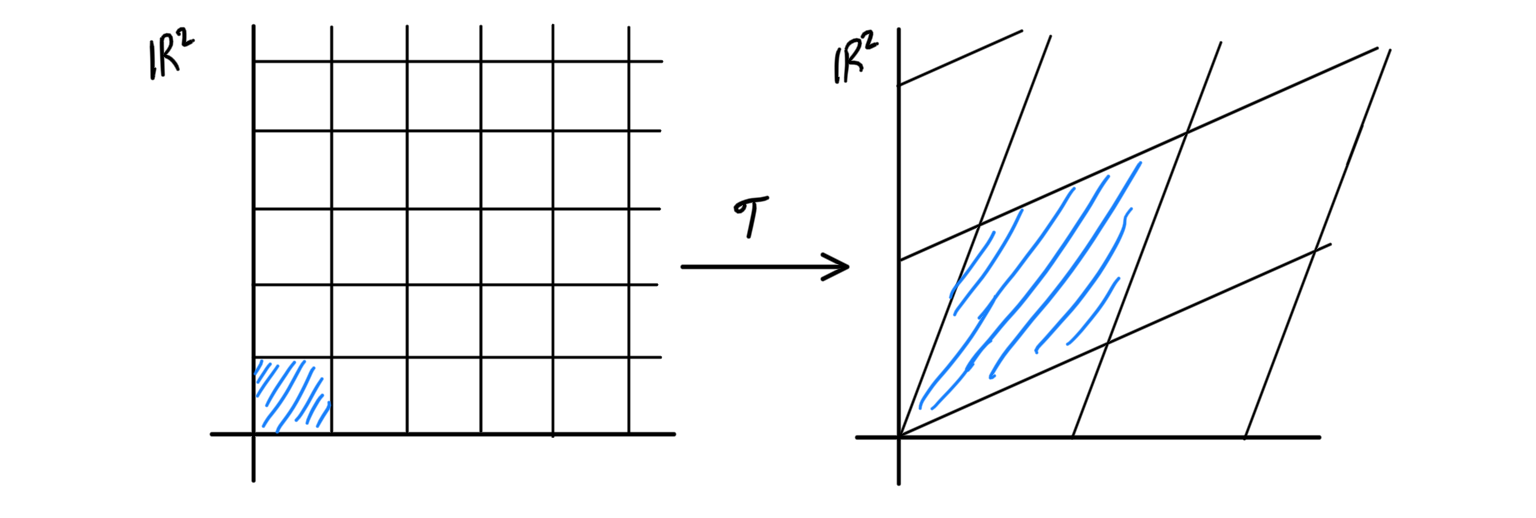
\includegraphics[scale=0.25]{Images/Determinant.PNG}
\end{center}

\begin{proposition}
The column vectors of $A$ are linearly dependent if and only if $\det{A} = 0$. 
\end{proposition}
\begin{proof}
By linearity, it is sufficient to prove that if two column vectors $a_i$ and $a_j$ of a matrix $A$ are equal, then $\det{A} = 0$. This can be easily seen by property (ii) of determinants. 
\end{proof}

\begin{theorem}
\[ \det{\bigg(\prod_i A_i \bigg)} = \prod_i \det{A_i}\]
\end{theorem}

\begin{theorem}
A matrix is invertible if and only if its determinant is nonzero. 
\end{theorem}
\begin{proof}
A matrix is invertible $\iff$ it is nonsingular $\iff$ its columns are linearly independent $\iff$ its determinant is nonzero, by the previous proposition. 
\end{proof}

\begin{corollary}
Given $n \times n$ matrix $A$,
\[\det{(A^{-1})} = \frac{1}{\det{A}}\]
\end{corollary}

\begin{theorem}
The determinants of similar matrices are equal. 
\end{theorem}
\begin{proof}
Let $A$ and $B$ be similar matrices. Then, there exists an $S$ such that $A = S^{-1} B S$ and 
\[ \det{(A)} = \det{(S^{-1} B S} = \det{(S^{-1})} \det{(B)} \det{(S)} = \det{B}\]
\end{proof}

This theorem implies that the determinant is an intrinsic property of a linear transformation, so it is invariant under a change of basis. That is, choosing different matrix representations of a linear transformation does not change the determinant.  

\begin{corollary}
\[\det{(A)} = \det{(A^T)}\]
\end{corollary}
\begin{proof}
$A$ is similar to $A^T$, which will be proven in chapter 6. 
\end{proof}

\begin{proposition}
The properties of the determinant combined with the previous corollary implies that 
\begin{enumerate}
    \item Adding a scalar multiple of a row/column to another row/column doesn't affect the determinant. 
    \item Interchanging two rows/columns switches the sign of the determinant. 
    \item Multiplying a row/column by $\alpha$ multiplies the determinant by $\alpha$. 
\end{enumerate}
\end{proposition}

\begin{theorem}
Let $A$ be an $n \times n$ matrix whose first column is $e_1$
\[A = \begin{pmatrix}
1&*&*&* \\
0 &&& \\
\ldots& & A_{11}& \\
0&&&
\end{pmatrix}\]
where $A_{11}$ is the $(n-1) \times (n-1)$ submatrix of $A$ with entries $a_{i j}, \; i, j > 1$. Given this, 
\[\det{A} = \det{A_{11}}\]
\end{theorem}
\begin{proof}
Using column reduction, we can see that 
\[ \det{A} = \det{\begin{pmatrix}
1&0&0&0 \\
0 &&& \\
\ldots& & A_{11}& \\
0&&&
\end{pmatrix}}\]
it is clear that the right hand side is equal to $\det{A_{11}}$ since it behaves exactly like $\det{A_{11}}$ with respect to the three properties. 
\end{proof}

\begin{corollary}
Let $A$ be an upper or a lower triangular matrix. Then the determinant of $A$ is the product of its diagonal entries. That is,  
\[ \det{A} = \prod_{i} a_{i i}\]
\end{corollary}
\begin{proof}
We apply the previous theorem recursively to satisfy when $A$ is upper triangular. Since $\det{(A)} = \det{(A^T)}$, this fact can be applied to lower triangular matrices too. 
\end{proof}

It is once again verified that the three elementary row (and column) operations affect the determinant in the way stated in Proposition 5.5. To elaborate, since $E_1, E_2$, and $E_3$ are all lower triangular, we can compute their determinants easily
\begin{align*}
    \det{E^1_{\alpha \times i + j}} = 1 \\
    \det{E^2_{i j}} = -1 \\
    \det{E^3_{\alpha \times i}} = \alpha
\end{align*}
and multiplying matrix $A$ by elementary matrices $E^1, E^2$, and $E^3$ multiplies the determinant by $1, -1$, and $\alpha$, respectively. 
\\

We can describe the determinant visually. Given a linear mapping $A: V \longrightarrow V$, we can fix any basis $\{e_1, e_2, ..., e_n\}$ on $V$. Note that these basis vectors do not need to be orthogonal, nor are they restricted to any magnitude. The set of vectors 
\[\Big\{ \sum_{i=1}^n c_i e_i \; | \; 0 \leq c_i \leq 1, i = 1, 2, ..., n\Big\}\]
forms an $n$-dimensional parallelepiped in $V$. Let the volume of this parallelepiped be $U$. Let $W$ be the volume of the parallelepiped 
\[\Big\{ \sum_{i=1}^n c_i A e_i \; | \; 0<c_i<1, i = 1, 2, ..., n\Big\}\]
which is formed by the transformed basis vectors $\{Ae_1, Ae_2, ..., Ae_n\}$. We can view this latter shape as the image of the first parallelepiped under transformation $A$. Then, 
\[ \det{A} = W / V \]
That is, the ratio of the transformed parallelepiped to the original parallelepiped is the determinant. This is consistent with the properties of the determinant. For example, if $A$ is not isomorphic, then the parallelepiped will get "squished" into a lower-dimensional parallelepiped with volume $0$. The fact that we use a ratio between the original and transformed parallelepiped allows this value to be invariant under the basis that we use. 

Computationally, finding the LUP decomposition of a matrix $A$ is the best known algorithm to compute the determinant of a general $n \times n$ matrix. That is, 
\[ \det{A} = \det{L} \det{U} \det{P} = \pm \det{U} = \pm \prod_i u_{i i}\]
since $\det{L} = 1$ and $\det{P} = \pm 1$. 

There are other methods to compute the determinant. First, we state the simple but useful formula.

\begin{proposition}
\[\det{\begin{pmatrix}
a&b\\c&d 
\end{pmatrix}} = a d - b c\] 
\end{proposition}

\begin{definition}
Given an $n \times n$ matrix $A$, the $(i j)$th minor of $A$, denoted $A_{i j}$, is the determinant of the $(n-1) \times (n-1)$ matrix formed by removing the $i$th row and $j$ th column from $A$. 
\end{definition}

\begin{theorem}[Laplace Expansion]
Let $A$ be an $n \times n$ matrix and $j$ any index between $1$ and $n$. Then
\[\det{A} = \sum_i (-1)^{i + j} a_{i j} A_{i j}\]
that is, the alternating sums of the $ij$th minors multiplied by the $ij$th entries in the $j$th column of $A$. This can be done by choosing an arbitrary $i$th row, which leads to the alternative formula 
\[\det{A} = \sum_j (-1)^{i + j} a_{i j} A_{i j} \]
\end{theorem}

\begin{theorem}[Cramer's Rule]
Given a system of linear equations in the form $A x = b$ where $A$ is an $n \times n$ matrix, the solutions of this system can be expressed with the formulas 
\[ x_i = \frac{ \det{A_i}}{\det{A}}\]
where $\det{A_i}$ is the matrix formed by replacing $a_i$, the $i$th column of $A$, by the column vector $b$. 
\end{theorem}

Albeit very computationally heavy, determinants can also be used to calculate the inverse of a matrix. 

\begin{theorem}
The inverse matrix $A^{-1}$ of an invertible matrix $A$ has the form 
\[(A^{-1})_{i j} = (-1)^{i+j} \frac{\det{A_{i j}}}{\det{A}}\]
\end{theorem}

\begin{definition}
The trace of a square matrix $A$, denoted $\Tr{A}$, is the sum of its diagonal entries. 
\[\Tr(A) = \sum_{i} a_{ii}\]
\end{definition}

\begin{proposition}
\[\Tr(\lambda A + \alpha B) = \lambda \Tr(A) + \alpha \Tr(B)\]
\end{proposition}
\begin{proof}
Obvious if we look at the entries of $A$ and $B$ and see that it is bilinear.
\end{proof}

\begin{theorem}[Cyclic Property of the Trace]
\[\Tr{\bigg(\prod_{i=1}^n A_i\bigg)} = \Tr{\bigg(A_n \prod_{i=1}^{n-1} A_i\bigg)}\]
\end{theorem}
\begin{proof}
We first prove when $m=2$. Given that the subscripts $i j$ denote that $(i,j)$th element of a matrix, observe that
\begin{align*}
    (AB)_{ij} = \sum_{k} A_{ik} B_{kj} & \implies (AB)_{ii} = \sum_{K} A_{ik} B_{ki} \\
    & \implies \Tr(AB) = \sum_{i} \sum_{k} A_{ik} B_{ki} \\
    & \;\;\;\;\;\;\;\;\;\;\;\;\;\;\;\;\;\;\;\;\;\;= \sum_{k} \sum_{i} B_{ki} B_{ik} = Tr(BA)
\end{align*}
Similarly, for $m=3$
\begin{align*}
    (ABC)_{ij} = \sum_{k,l} A_{ik} B_{kl} C_{lj} & \implies \Tr(ABC) = \sum_{i,k,l} A_{ik} B_{kl} C_{li} \\ 
    & \;\;\;\;\;\;\;\;\;\;\;\;\;\;\;\;\;\;\;\;\;\;\;\;\;= \sum_{i,k,l} C_{li} A_{ik} B_{kl} = \Tr(CAB)
\end{align*}
And so we can generalize for $m$. 
\end{proof}

\begin{corollary}
The trace is invariant under a change of basis. That is, the trace is an intrinsic property of a linear transformation since it does not change depending on how it is represented. 
\end{corollary}
\begin{proof}
Given that $A$ is similar to $B$. 
\[\Tr(B) = \Tr(S A S^{-1}) = \Tr(S^{-1} S A) = \Tr(A) \]
\end{proof}

\begin{theorem}
Let $A$ be a $n \times n$ skew-symmetric matrix over $\mathbb{C}$ (or any field of characteristic $\neq 2$). If $n$ is odd, 
\[\det{A} = 0 \]
\end{theorem}
\begin{proof}
\[\det{A} = \det{A^T} = \det{-A} = (-1)^n \det{A} \implies \det{A} = 0 \]
\end{proof}

We can actually conclude something even futher about antisymmetric matrices. 

\begin{theorem}
The determinant of an antisymmetric matrix $A$ of even order is the square of a homogeneous polynomial of degree $n/2$ in the entries of $A$. That is, 
\[\det{A} = P^2\]
The polynomial $P$ is called the \textit{Pfaffian}. 
\end{theorem}

\begin{definition}
A \textit{Vandermonde matrix} is a square matrix whose columns form a geometric progression. That is, let $a_1, a_2, ..., a_n$ be $n$ scalars. Then, $V(a_1, a_2, ..., a_n)$ is the $n \times n$ matrix
\[\begin{pmatrix}
1&1&\ldots&1&1 \\
a_1&a_2&\ldots&a_{n-1}&a_n\\
\vdots&\vdots&\ddots&\vdots&\vdots\\
a_1^{n-2}&a_2^{n-2}&\ldots&a_{n-1}^{n-2}&a_n^{n-2}\\
a_1^{n-1}&a_2^{n-1}&\ldots&a_{n-1}^{n-1}&a_n^{n-1}
\end{pmatrix}\]
\end{definition}

\begin{theorem}
The determinant of a Vandermonde matrix is
\[\det{V(a_1, a_2, ..., a_n)} = \prod_{j>i} (a_j - a_i)\]
\end{theorem}

A symmetry in the multivariable expression of a determinant can also reveal a symmetry in the matrix.

\begin{example}[2019 Putnam A1]
The symmetric polynomial 
\[ f(x, y, z) = x^3 + y^3 + z^3 - 3 x y z\]
can be expressed as the determinant of the $3 \times 3$ matrix
\[\det{\begin{pmatrix}
x&y&z\\
z&x&y\\
y&z&x
\end{pmatrix}}\]
\end{example}

\subsection{Matrices in Block Form}
\begin{theorem}
Given $2 \times 2$ block matrices
\[X = \begin{pmatrix}
A_1&B_1\\C_1&D_1
\end{pmatrix}, \; \; Y = \begin{pmatrix}
A_2&B_2\\C_2&D_2
\end{pmatrix}\]
We can compute $X Y$ similarly to regular matrix multiplication, treating the blocks as entries. 
\[ X Y = \begin{pmatrix}
A_1&B_1\\C_1&D_1
\end{pmatrix} \begin{pmatrix}
A_2&B_2\\C_2&D_2
\end{pmatrix} = \begin{pmatrix}
A_1 A_2 + B_1 C_2 & A_1 B_2 + B_1 D_2 \\
C_1 A_2 + D_1 C_2 & C_1 B_2 + D_1 D_2 
\end{pmatrix}\]
Furthermore, this process can be done in general for any $m \times n$ block matrix $X$ and $n \times p$ block matrix $Y$. 
\end{theorem}

\begin{theorem}
Given that $I_N, A, B$ are $n \times n$ matrices, define the $(2n) \times (2n)$ matrix 
\[X = \begin{pmatrix}
I & 0 \\ A & B
\end{pmatrix}\]
Then 
\[\det{X} = \det{B}\]
\end{theorem}
\begin{proof}
We can perform Gauss elimination to reduce $X$ without affecting the determinant.
\[\det{\begin{pmatrix}
I&0\\A&B
\end{pmatrix}} = \det{
\begin{pmatrix}
I&0\\
0&B
\end{pmatrix}} = \det{B}\]
since it satisfies the correct properties for $\det{B}$. 
\end{proof}

\begin{corollary}
\[\det{\begin{pmatrix}
A&0\\C&D
\end{pmatrix}} = \det{A} \det{D}\]
\end{corollary}

\begin{proof}
\[ \det{\begin{pmatrix}
A&0\\C&D 
\end{pmatrix}} = \det{\begin{pmatrix}
A&0\\C&I
\end{pmatrix} \begin{pmatrix}
I&0\\0&D
\end{pmatrix}} = \det{\begin{pmatrix}
A&0\\C&I
\end{pmatrix}} \det{\begin{pmatrix}
I&0\\0&D
\end{pmatrix}}\]
\end{proof}

However, 
\[\det{\begin{pmatrix}
A&B\\C&D
\end{pmatrix}} \neq \det{A} \det{D} - \det{B} \det{C}\]

Rather, we introduce the following theorem

\begin{theorem}
\begin{align}
    \det{\begin{pmatrix} A&B\\C&D \end{pmatrix}}  & = \det{(A)} \det{(D - C A^{-1} B)} \\
    & = \det{(D)} \det{(A - B D^{-1} C)}
\end{align}
\end{theorem}
\begin{proof}
\[\begin{pmatrix} A&B\\C&D\end{pmatrix} = \begin{pmatrix}
A&0\\C&I\end{pmatrix} \begin{pmatrix}
I& A^{-1} B \\ 0 & D - C A^{-1} B
\end{pmatrix}\]
by similarity, equation $(6)$ is equal to equation $(7)$. 
\end{proof}

\begin{definition}
A \textit{block diagonal matrix} is a square matrix in block form such that the diagonal blocks are square matrices and all off-diagonal blocks are zero matrices. 
\[A = \begin{pmatrix}
A_1&0&\ldots&0\\
0&A_2&\ldots&0\\
\vdots&\vdots&\ddots&\vdots\\
0&0&\ldots&A_k
\end{pmatrix}\]
\end{definition}

\begin{theorem}
Given a matrix $A$ in block diagonal form, with diagonal blocks $A_1, A_2, ..., A_k$,
\[\det{A} = \prod_{i=1}^k A_i, \; \; \Tr{A} = \sum_{i=1}^k \Tr{A_i}\]
Furthermore, $A$ is invertible if and only if all the $A_i$'s are invertible, and 
\[A^{-1} = \begin{pmatrix}
A_1&0&\ldots&0\\
0&A_2&\ldots&0\\
\vdots&\vdots&\ddots&\vdots\\
0&0&\ldots&A_k
\end{pmatrix} = \begin{pmatrix}
A_1^{-1}&0&\ldots&0\\
0&A_2^{-1}&\ldots&0\\
\vdots&\vdots&\ddots&\vdots\\
0&0&\ldots&A_k^{-1}
\end{pmatrix}\]
\end{theorem}
\begin{proof}
The results are obvious when performing block multiplication or Gauss Elimination. 
\end{proof}

\subsection{Dodgson Condensation}
We already know that the LUP decomposition is an algorithm used to compute the determinant of a general $n \times n$ matrix. We will introduce another, called \textit{Dodgson condensation}. The algorithm can be described in the following steps.

\begin{enumerate}
    \item Let $A$ be a given $n \times n$ matrix. Arrange $A$ so that no zeros occur in its interior (this can be done by any combination of elementary row or column operations that would not change the determinant). 
    \item Create an $(n-1) \times (n-1)$ matrix $B$ consisting of the determinants of every $2 \times 2$ submatrix of $A$. Explicitly, 
    \[B = \det{\begin{pmatrix}
    a_{i,j} & a_{i,j+1} \\ a_{i+1,j} & a_{i+1,j+1}
    \end{pmatrix}}\]
    \item With this $(n-1) \times (n-1)$ matrix $B$, perform step $2$ to obtain an $(n-2) \times (n-2)$ matrix $C$. Divide each term in $C$ by the corresponding term in the interior of $A$. 
    \[C_{i,j} = \det{\begin{pmatrix}
    b_{i,j} & b_{i,j+1} \\ b_{i+1,j} & b_{i+1,j+1}
    \end{pmatrix}} \bigg/ a_{i+1,j+1}\]
    \item Let $A = B$ and $B=C$. Repeat step $3$ as necessary until the $1 \times 1$ matrix is found, which is the determinant. 
\end{enumerate}

The reason that we do not want $0$s in $A$ is because then in doing step $3$ we may divide by $0$. 

\begin{example}
Let us find
\[\det{\begin{pmatrix}
-2&-1&-1&-4\\-1&-2&-1&-6\\-1&-1&2&4\\2&1&-3&-8
\end{pmatrix}}\]
All of the interior elements are nonzero, so there is no need to rearrange the matrix. We calculate
\[\begin{pmatrix}
-2&-1&-1&-4\\-1&-2&-1&-6\\-1&-1&2&4\\2&1&-3&-8
\end{pmatrix} \rightarrow \begin{pmatrix}
3&-1&2\\-1&-5&8\\1&1&-4
\end{pmatrix} \rightarrow \begin{pmatrix}
-16&2\\4&12
\end{pmatrix}\]
With this $2 \times 2$ matrix, we must divide each term by the interior of the original $A$. 
\[\begin{pmatrix}
-16/-2 & 2/-1\\4/-1 & 12/2
\end{pmatrix} = \begin{pmatrix}
8&-2\\-4&6
\end{pmatrix}\]
Calculating this determinant gives $40$, and dividing by the interior of the $3 \times 3$ matrix $(-5)$ gives $\det{A} = 40/-5 = -8$. 
\end{example}

\subsection{Matrix Calculus}
There is nothing special about matrix calculus on its own, since matrices are themselves vectors; they can be sufficiently analyzed using vector calculus. Regardless, we will emphasize a few points. Let
\[A: \mathbb{R} \longrightarrow \text{Mat}(m \times n, \mathbb{R})\]
be a matrix valued differential function. That is, the $m \times n$ component functions of $A$ is differentiable. Then, just like in calculus, we introduce differentiation rules.
\begin{align*}
    & \frac{d}{d x} \big( A(t) + B(t)\big) = \frac{d}{d t} A(t) + \frac{d}{d t} B(t) \\
    & \frac{d}{d x} \big( c A(t)\big) = c \frac{d}{d t} A(t)
\end{align*}
The scalar multiplication can actually be extended. By linearity (of matrix multiplication), we can say that if $A$ is independent of $t$, then 
\[\frac{d}{d x} A B (x) = A \frac{d}{d x} B(x)\]
The linearity of the derivative allows us to state more rules. Given that $v: \mathbb{R}^n \longrightarrow \mathbb{R}$ is a scalar valued function and $l \in (\mathbb{R}^n)^*$, then  
\[\frac{d}{d x} l \big( v(x) \big) = l \bigg( \frac{d}{d x} v(x) \bigg)\]
This result can be extended to when $v$ is replaced by matrix valued function $A$ and $l$ is replaced by $\phi: \text{Mat}(m \times n, \mathbb{R}) \longrightarrow \mathbb{R}$. 
\[\frac{d}{d x} \phi \big( A(x) \big) = \phi \bigg( \frac{d}{d x} A(x) \bigg)\]
Since the trace is a linear operator, we have the following theorem. 

\begin{theorem}
Given a linear function $A: \mathbb{R} \longrightarrow \text{Mat}(n, \mathbb{R})$ with paramater $x$, 
\[\frac{d}{d x} \Tr{A} = \Tr \bigg( \frac{d}{d x} A \bigg)\]
Note that $A$ in here really means $A(x)$.
\end{theorem}

The product rule of matrix calculus is similar.
\[\frac{d}{d x} A B = \bigg(\frac{d}{d x} A\bigg) \cdot B + A \cdot \bigg(\frac{d}{d x} B \bigg)\]
It is also noting that the derivative of the inner product of two vector valued functions $v, w: \mathbb{R} \longrightarrow \mathbb{R}^n$ is 
\[\frac{d}{d x} \big( v(x), w(x) \big) = \Big( \frac{d}{d x} v(x), w(x) \Big) + \Big( v(x), \frac{d}{d x} w(x) \Big)\]

\begin{definition}
A matrix valued function $A$ is \textit{invertible at a point $x \in \mathbb{R}$} if there exists a function, denoted $A^{-1}$ such that
\[A(x) A^{-1} (x) = A^{-1}(x) A(x) = I\]
where $I$ is the identity matrix. If there exists such $A^{-1}$ for all values $x \in \mathbb{R}$, then $A$ is said to be \textit{invertible}. 
\end{definition}

\begin{theorem}
Let $A$ be a matrix valued function, differentiable and invertible. Then, the function $A^{-1}$ is also differentiable and 
\[\frac{d}{d x} A^{-1} = - A^{-1} \bigg( \frac{d}{d x} A \bigg) A^{-1}\]
\end{theorem}
\begin{proof}
We derive this using the product rule. 
\begin{align*}
    0 = \frac{d}{d x} I & = \frac{d}{d x} \big( A(x) A^{-1} (x) \big) \\
    & = A(x) \bigg(\frac{d}{d x} A^{-1} (x) \bigg) + \bigg( \frac{d}{d x} A(x) \bigg) A^{-1} (x) \\
    \implies \frac{d}{d x} A^{-1} (x) & = - A^{-1} (x) \bigg( \frac{d}{d x} A(x) \bigg) A^{-1}(x)
\end{align*}
\end{proof}
Note that the chain rule is a rule of differentiaion that applies for scalar valued functions. That is, given $f: V \longrightarrow \mathbb{R}$ and $g: \mathbb{R} \longrightarrow V$ ($V$ vector space), 
\[\frac{d}{d x} f \circ g (x) = f^\prime \big( g(x) \big) \cdot \frac{d}{d x} g(x)\]
The $\cdot$ operation in the right hand side is the operation of multiplication in the field $\mathbb{R}$. But given $f: \text{Mat}(n, \mathbb{R}) \longrightarrow \mathbb{R}$ and $A \mathbb{R} \longrightarrow \text{Mat}(n, \mathbb{R})$, multiplication within the algebra of matrices are inherently different than component-wise operations, so the chain rule does not apply (it would apply if matrix multiplication was defined component-wise). 

\begin{example}
Let $f(A) \equiv A^2$, and let $A$ be a matrix valued function. Then, 
\begin{align*}
    \frac{d}{d x} f \circ A(x) = \frac{d}{d x} \big( A(t) \big)^2 & = \bigg( \frac{d}{d x} A(x) \bigg) \cdot A(x) + A(x) \cdot \bigg( \frac{d}{d x} A(x) \bigg) \\
    & \neq 2 A(x) \cdot \frac{d}{d x} A(x)
\end{align*}
since matrix multiplication is in general not commutative. 
\end{example}

\begin{proposition}
\[\frac{d}{d x} A^k = A^\prime A^{k-1} + A A^\prime A^{k-2} + ... + A^{k-2} A^\prime A + A^{k-1} A^\prime\]
\end{proposition}
\begin{proof}
We inductively apply the product rule
\[\frac{d}{d x} A^k = A^\prime A^{k-1} + A \frac{d}{d x} A^{k-1}\]
\end{proof}

\begin{corollary}
Given any polynomial $p$ with $A$ a differentiable, square matrix valued function, if $A$ and $A^\prime$ commute, then 
\[\frac{d}{d x} p(A) = p^\prime (A) A^\prime\]
\end{corollary}
\begin{proof}
We can completely define differentiation over the vector space of polynomials with the formula
\[\frac{d}{d x} A^k = k A^{k-1} A^\prime \; \forall k \in \mathbb{N}\]
\end{proof}

\begin{corollary}
Given polynomial $p$ with $A$ a differentiable, square matrix valued function, 
\[\frac{d}{d x} \Tr{p(A)} = \Tr{\big( p^\prime(A) \cdot A^\prime \big)}\]
\end{corollary}
\begin{proof}
Use the cyclic trace property.
\end{proof}

\begin{definition}
The \textit{exponential map} is defined
\[\text{exp}: \text{Mat}(n, \mathbb{C}) \longrightarrow \text{Mat}(n, \mathbb{C})\]
where 
\[e^A = I + A + \frac{1}{2!} A^2 + \frac{1}{3!} A^3 + ... = \sum_{k=0}^\infty \frac{1}{k!} A^k\]
where $A^0 \equiv I$. This can clearly be extended to when $A$ is a square, matrix valued function. 
\end{definition}

This final theorem establishes the connection between the determinant and trace. 

\begin{theorem}
Given a differentiable square matrix valued function $A$ such that $A$ is invertible for a certain $x \in \mathbb{R}$, then 
\[\frac{d}{d x} \log{\det{A}} = \Tr \bigg( A^{-1} \frac{d}{d x} A \bigg)\]
Where the log mapping is the inverse of the exponential mapping of matrices. 
\end{theorem}

\begin{definition}
The \textit{commutator} in the algebra of $n \times n$ matrices is defined as 
\[[A, B] = A B - B A\]
\end{definition}

\begin{theorem}
If $A$ and $B$ are commuting square matrices, then 
\[e^{A + B} = e^A \, e^B\]
In general, the solution $C$ to the equation
\[e^{A} \, e^B = e^C\]
is given by the \textit{Baker-Campbell-Hausdorff formula}, defined
\[C = A + B + \frac{1}{2}[A,B] + \frac{1}{12} [A,[A,B]] - \frac{1}{12} [B,[A,B]] + ...\]
consisting of terms involving higher commutators of $A$ and $B$. The full series is much too complicated to write, so we ask the reader to be satisfied with what is shown. 
\end{theorem}

\begin{corollary}
\[\Tr{\log{e^A \, e^B}} = \Tr{A} + \Tr{B}\]
\end{corollary}

\section{Spectral Theory} 
\subsection{Spectral Theory of General Mappings}
\begin{definition}
Let $A: V \longrightarrow V$ be a linear transformation over $\mathbb{F}$. If there exists a vector $v \in V$ such that
\[ A v = \lambda v, \; \lambda \in \mathbb{F}\]
then $a$ is called an \textit{eigenvalue} of $A$, and $v$ is an \textit{eigenvector} of $A$. Clearly, if a basis is realized for $V$ and $A$ is represented as a matrix, $v$ would have a basis representation. However, the value of $\lambda$ is invariant. The set of all eigenvalues 
\[\lambda(A) \equiv \{ \lambda_1, \lambda_2, ..., \lambda_k\}\]
is called the \textit{spectrum} of $A$. 
\end{definition}

\begin{remark}
For a given eigenvalue $\lambda$ and its corresponding eigenvector $v$, it is clear that by linearity, every vector in $\Span v$ is an eigenvector, too. 
\end{remark}

Now that we have defined eigenvalues and eigenvectors, we first provide a visual description of these terms. Given a linear transformation $A: V \longrightarrow V$, we can visualize a certain basis of $V$ such that all the linear transformation $A$ does on that basis is merely extend or contract the basis vectors.

\begin{definition}
Given a $n \times n$ matrix $A$, the \textit{characteristic polynomial} of $A$, denoted $p_A (t)$, is defined
\[ p_A (t) \equiv \det{(A - t I)}\]
The mapping $A \mapsto p_A (t)$ can be thought of as a mapping from Mat$(n, \mathbb{F}) \longrightarrow \mathbb{F}[t]$, where Mat$(n, \mathbb{F})$ is the algebra of $n \times n$ matrices over field $\mathbb{F}$, and $\mathbb{F}[t]$ is the polynomial algebra over $\mathbb{F}$. $p_A (t)$ is invariant under matrix similarity. 
\end{definition}

The motivation for defining such a polynomial is that it allows us to compute the eigenvalues of $A$. 
\begin{definition}
The \textit{characteristic equation} of $A$ is defined by equating $p_A (t) = 0$. 
\end{definition}

\begin{proposition}
The solutions of the characteristic equation of $A$ (i.e. the roots of $p_A (t)$) is precisely the spectrum of $A$. 
\end{proposition}

\begin{proof} $(\rightarrow)$ Let there be a $t = \lambda$ such that $p_A (\lambda) = 0 \iff \det{(A - \lambda I)} = 0$ which is equivalent to saying that ker$(A - \lambda I)$ is nontrivial. There must exist a $v \in $ ker$(A - \lambda I)$, meaning that $(A - \lambda I) v = 0 \iff A v = \lambda v$. By definition, $\lambda$ is an eigenvalue of $A$. \\
$(\leftarrow)$ This reasoning can be extended in the opposite direction. 
\end{proof}

\begin{theorem}
Eigenvectors of a linear transformation $A$ corresponding to different eigenvalues are linearly independent, but not necessarily orthogonal. It follows that if the characteristic polynomial of a $n \times n$ matrix $A$ has $n$ distinct roots, then $A$ has $n$ linearly independent eigenvectors. 
\end{theorem}

\begin{proof}
Simple, by contradiction.
\end{proof}

\begin{example}
It is clear that the Fibonacci sequence can be produced with matrix multiplication as such 
\[ \begin{pmatrix}
a_{n+1} \\ a_n
\end{pmatrix} = A^n \begin{pmatrix}
a_1 \\ a_0
\end{pmatrix} = \begin{pmatrix}
1&1\\1&0
\end{pmatrix}^n \begin{pmatrix}
1\\1
\end{pmatrix}\]
Given that 
\[\lambda_1 = \frac{1+\sqrt{5}}{2}, \; \lambda_2 = \frac{1 - \sqrt{5}}{2}\]
we can diagonalize $A$ into the form 
\[A = \begin{pmatrix}
\frac{1}{\lambda_1 - \lambda_2} & \frac{\lambda_2}{\lambda_2 - \lambda_1} \\
\frac{1}{\lambda_2 - \lambda_1} & \frac{\lambda_1}{\lambda_1 - \lambda_2}
\end{pmatrix} \begin{pmatrix}
\lambda_1 & 0 \\ 0 & \lambda_2 
\end{pmatrix} \begin{pmatrix}
\lambda_1 & \lambda_2 \\
1 & 1
\end{pmatrix} \implies A^n = S^{-1} \begin{pmatrix}
\lambda_1^n & 0 \\ 0 & \lambda_2^n 
\end{pmatrix} S\]
which implies that after evaluating, we get 
\[ a_n = \frac{1}{\sqrt{5}} \bigg( \Big(\frac{1+\sqrt{5}}{2}\Big)^n - \Big(\frac{1-\sqrt{5}}{2}\Big)^n \bigg)\]
This is a surprising result since it also says that the expression above is always an integer for all natural number $n$. 
\end{example}
\begin{definition}
Given a subspace $U_1 \subset U$ and linear transformation $T: U \longrightarrow U$. We say that $U_1$ is \textit{invariant} under $T$ if 
\[u \in U_1 \implies T u \in U_1\]
\end{definition}

\begin{theorem} 
Let $a_1, a_2, ..., a_n$ be the eigenvalues of $A$. Then 
\[\sum_i a_i = \Tr{A}, \;\;\; \prod_i a_i = \det{A}\]
\end{theorem}

\begin{proof}
The mapping $A \mapsto \det{(A - x I)}$ is a mapping from the set of $n \times n$ matrices to the polynomial algebra $\mathbb{F}[x]$. Direct application of the Viete's formulas in $\mathbb{F}[x]$ produces the statement and this result can be extended to the rest of the formulas. 
\end{proof}

\begin{theorem}[Spectral Mapping Theorem]
Let $q$ be any polynomial, $A$ a square matrix with an eigenvalue $a$. Then: 

i) $q(a)$ is an eigenvalue of $q(A)$. 

ii) Every eigenvalue $q(A)$ is of the form $q(a)$, where $a$ is an eigenvalue of $A$. 
\end{theorem}
\begin{proof} 
i) Let $h$ be an eigenvector of A with corresponding eigenvalue $a$. 
\begin{align*}
    Ah = ah & \implies A^{2} h = Aah = aAh = a^{2} h \\
 & \implies A^{n} h = a^{n} h   \\
 & \implies q(A)h = q(a)h \\
 & \implies q(a) \text{ is an eigenvalue of }q(A)
\end{align*}
ii) Let $p$ be the eigenvalue of $q(A) \iff \det{\big(q(A) - p I\big)} = 0$. We expand: 
$$ q(s) - p = c\prod \big(s-r_{i}\big), r_{i} \in \mathbb{C} $$ 
Replacing the variable $s$ with $A$, we have
$$ q(A) - pI = c \prod \big(A-r_{i}I\big) $$
Since $\det{\big( q(A) - pI\big)} = 0$, at least one $r_{i}$, say $r_{k}$ exists such that $\det{\big( A - r_{k} I \big)} = 0 \iff r_{k}$ is an eigenvalue of $A$. Since $q(r_{j})-p = 0$, $p = q(r_{j})$ is an eigenvalue of $q(A)$. 
\end{proof}

The following theorem is an equivalent version of the spectral mapping theorem.
\begin{theorem}
Let $A$ be a $n \times n$ matrix and let $f$ be a polynomial. If the chracteristic polynomial of $A$ has factorization 
\[p_A (t) = \prod_{i = 1}^n (t - \lambda_i)\]
then the characteristic polynomial of the matrix $f(A)$ is given by 
\[p_{f(a)} (t) = \prod_{i = 1}^n (t - f(\lambda_i))\]
\end{theorem}

We can actually create a bound on the spectrum of a square matrix. 

\begin{theorem}[Gershgorin Circle Theorem]
Let $A \in $ Mat$(n, \mathbb{C})$ with entries $a_{i j}$. Let $R_i = \sum_{i \neq j} |a_{i j}|$ be the sum of the absolute values of the non-diagonal entries of the $i$th row, and let $D_(a_{i i}, R_i) \subset \mathbb{C}$ be a closed disk with radius $R_i$ centered at $a_{i i}$ in the complex plane, called a \textit{Gershgorin Disk}. Then every eigenvalue of $A$ lies within the union of all $n$ Gershgorin Disks. That is, 
\[ \lambda_j (A) \in \bigcup_{i= 1}^{n} D_(a_{i i}, R_i) \subset \mathbb{C}, \text{ for all } j\]
\end{theorem}

\begin{proof}
Let $\lambda$ be an eigenvalue of $A$ with its eigenvector $v = (v_j)$. Scale $v$ by multiplying it by $ \pm 1 / \max{\{|v_j|\}_j}$ to get a vector $x$ with its maximal entry $x_i = 1$ and $|x_j| \leq 1, \; j \neq i$. Then, 
\[A x = \lambda x \implies \sum_{j} a_{i j} x_j = \lambda x_i = \lambda \implies \sum_{j \neq i} a_{i j} x_j + a_{i i} = \lambda\]
Applying the triangle inequality, 
\[| \lambda - a_{i i} | = \bigg| \sum_{j \neq i} a_{i j} x_j\bigg| \leq \sum_{j \neq i} |a_{i j}| |x_j| \leq \sum_{j \neq i} |a_{i j}| = R_i\]
\end{proof}

\begin{corollary}
The eigenvalues of $A$ must also lie within the Gershgorin discs $C_j$ corresponding to the columns of $A$. 
\end{corollary}

\begin{proof}
This is a direct result from the fact that $A$ is similar to $A^T$. Alternatively, we can apply the same process in the proof above to $A^T$.
\end{proof} 

If one observes that the off-diagonal entries of $A$ are small in absolute value, it can be concluded that the diagonal entries are "close" to the true eigenvalues of $A$. $A$ is diagonal if and only if the Gershgorin disks are points. 

\begin{theorem}[Cayley Hamilton]
Every matrix $A$ satisfies its own characteristic equation. That is, 
\[ p_{A}(A) = 0\]\
\end{theorem} 

\subsection{Eigendecompositions and Jordan Normal Form}

However, the entire concept of matrices are not fully grasped with just eigenvectors. If it were, then linear algebra would be a much simpler matter. To extend our toolkit, we must introduce generalized eigenvectors. From here, we will assume that our field is over $\mathbb{C}$. We use the fact that the field is over $\mathbb{C}$ because it allows us to claim that the characteristic polynomial in $\mathbb{C}[t]$ can be factored into linear components, by the fundamental theorem of algebra. 

\begin{definition}
A genuine eigenvector of $A$ satisfies $(A-aI)h = 0$. A \textit{generalized eigenvector} $f$ satisfies $(A-a I)^{d} f = 0$ for some $d \geq 1$. 
\end{definition}

To provide a visual intuition of how generalized eigenvectors transform under $A$, observe that 
\begin{align}
    (A - aI) h = 0 \text{ and } (A - aI)^2 f = 0 & \implies (A - aI)^f = h \\
    & \implies A f = a f + h, \; Ah = ah \\
    & \implies A^2 f = a A f + A h = a^2 f + 2 a h \\
    & \implies A^N f = A^N f + N a^{N-1} h 
\end{align}
This implies that the generalized eigenvector is first scaled by a factor of $a$, similar to a genuine eigenvector, but then a factor of the genuine eigenvector is then added to the scaled generalized one. Note that in higher dimensions of $N$, a greater multiple of $h$ must be added after scaling $f$. 

This means that given an eigenvalue $\lambda$, there is always at least one genuine eigenvalue associated with $\lambda$. Furthermore, there may be additional generalized eigenvectors also corresponding to $\lambda$. This leads to the following definition

\begin{definition}
The subspace formed by the span of the generalized (and genuine) eigenvectors of $\lambda$ form what is called the \textit{eigenspace associated with $\lambda$}, denoted $E(\lambda)$. 
\end{definition}

We can measure the characteristics of the eigenspaces with the following definitions. 

\begin{definition}
The \textit{algebraic multiplicity} of an eigenvalue $\lambda$ is the dimension of its eigenspace. It is precisely
\[\dim{E(\lambda)}\]  
In order to compute the algebraic multiplicity of $\lambda_i$ in $A$, we find the maximal value of $d_i$ such that $(t-\lambda)^{d_i}$ divides $p_A (t)$. With this, we can define 
\[E(\lambda) = \ker{(A - \lambda_i I)^{d_i}}\]
\end{definition} 

\begin{theorem}
Given $A: V \longrightarrow V$ with eigenspaces $E(\lambda_1), E(\lambda_2), ..., E(\lambda_k)$, 
\[E(\lambda_1) \oplus E(\lambda_2) \oplus ... \oplus E(\lambda_k) = V\]
That is, every vector $v \in V$ can be uniquely expressed as the sum 
\[ v = h_1 + h_2 + ... + h_k, \; h_i \in E(\lambda_i)\]
this is called the \textit{eigenbasis of $V$}. 
\end{theorem}
\begin{proof}
The definition of algebraic multiplicity implies that each eigenspace is disjoint except at $0$ and that their dimensions sum to $\dim{V}$. 
\end{proof}

\begin{definition}
The \textit{geometric multiplicity} of an eigenvalue $\lambda$ of a linear transformation $A$ is the dimension of the span of genuine eigenvectors in its eigenspace. It is precisely 
\[\dim{\ker{(A - \lambda I)}}\]
Note that since the span of genuine eigenvectors is a subspace of $E(\lambda)$, the geometric multiplicity is always less than or equal to the algebraic multiplicity. 
\end{definition}

Now we are ready to introduce the eigendecomposition of a linear mapping $A$.

\begin{theorem}
Given a linear mapping $A$ with its eigenvalues $\lambda_1, \lambda_2, ..., \lambda_k$ and associated eigenspaces $E(\lambda_1), E(\lambda_2), ..., E(\lambda_k)$, $A$ maps each eigenspace to itself. That is, 
\[A\big( E(\lambda_i) \big) \subset E(\lambda_i), \; i = 1, 2, ..., k\]
\end{theorem}

\begin{corollary}[Jordan Normal Form]
Every linear mapping $A: V \longrightarrow V$ can be decomposed into the sum of the linear mappings of each eigenspace $E(\lambda_i)$. That is, it can be expressed in the form 
\[A: \prod_i E(\lambda_i) \longrightarrow \prod_i E(\lambda_i)\]
which we can define, given $h_i \in E(\lambda_i)$, 
\[A(v) = A\bigg(\sum_i h_i \bigg) = \sum_i A(h_i), \; A(h_i) \in E(\lambda_i) \]
\end{corollary}

The process of eigendecomposition for a linear mapping $A$ is really just a clever change of basis for the $n \times n$ matrix representation of $A$ over $\mathbb{C}$, where the new basis is now the set of genuine and generalized eigenvectors. The new matrix formed by performing the change of basis on matrix $A$ is called the \textit{Jordan Normal Form}, or \textit{Jordan Canonical Form}, of $A$. We will now describe the construction of the JNF of an arbitrary $n \times n$ matrix. 

It is actually simple. Let the eigenvalues of the matrix $A$ be $\lambda_1, \lambda_2, ..., \lambda_k$, with its associated eigenspaces $E(\lambda_i)$. Let the algebraic multiplicity of eigenspace $E(\lambda_i)$ be $alg_i$. Then, every $n \times n$ matrix over $\mathbb{C}$ has the block form 
\[ J = \begin{pmatrix}
A_1&0&0&0\\
0&A_2&0&0\\
0&0&...&0\\
0&0&0&A_k
\end{pmatrix}\]
where each block $A_i$ represents the transformation in $E(\lambda_i)$. This means that each $A_i$ must be an $alg_i \times alg_i$ submatrix. The definition of the generalized eigenvectors shown in equation $(11)$ shows that each block must be of form 
\[A_i = \begin{pmatrix}
\lambda_i & 1 & 0 & ... & 0\\
0 &\lambda_i & 1 &...&0 \\
0&0&\lambda_i&...&0\\
...&...&...&...&1\\
0&0&...&0&\lambda_i
\end{pmatrix}\]
With $\lambda_i$'s in the main diagonal and $1$'s in the superdiagonal of $A_i$. The first column of $A$ refers to the transformation of the genuine eigenvector, while the other columns refers to the transformation of the generalized eigenvectors, where $\lambda_i$ refers to the scaling of the $d$th generalized eigenvector and the $1$ refers to the adding of the $(d-1)$th generalized eigenvector to the scaled $d$th vector. If there are no generalized eigenvectors in an eigenspace $E(\lambda_i)$, then $A_i$ is a $1 \times 1$ matrix $( \lambda_i )$. Observe that this form is consistent with our previous theorems, especially the fact that $A$ maps distinct eigenspaces to themselves. 

Finally, the change of basis is represented through the matrix multiplication. 
\[J = P^{-1} A P, \; P = \begin{pmatrix}
|&|&|&| \\ 
f_1&f_2&...&f_n \\
|&|&|&|
\end{pmatrix} \]
where $f_i$ is the genuine/generalized eigenvectors corresponding to the transformation represented in the $i$th column of $J$. The Jordan Normal Form of a matrix is unique up to the permutations of its diagonal blocks. 

Notice that the Jordan Normal Form must be an $n \times n$ matrices over $\mathbb{C}$, not $\mathbb{R}$. However, given a matrix $A$ over $\mathbb{R}$, we can construct a similar block diagonal form over $\mathbb{R}$. Since $A$ is real $\implies p_A (t) \in \mathbb{R}[t]$, $\mu \in \mathbb{C}$ is a root of $p_A$ implies that $\bar{\mu}$ is also a root. This means that in the case where $\mu = a \pm b i$ is a pair of complex eigenvectors with eigenvectors $z$ and $\bar{z}$. The associated $2 \times 2$ Jordan block will be of form
\[\begin{pmatrix}
a&-b\\ b&a
\end{pmatrix}\]
with the associated column vectors in $P$ being
\[v_1 = \frac{z + \bar{z}}{2}, \; v_2 = \frac{i (z - \bar{z})}{2}\]
Notice that $z \in \mathbb{C}^n$ is a complex eigenvector belonging to complex eigenvalue $\mu$, and we make the best "approximations" of $z, \bar{z}$ and $\mu, \bar{\mu}$ with the new real vectors $v_1$ and $v_2$. Note that the Jordan block states that
\[A(v_1) = a v_1 + b v_2, \; A(v_2) = -b v_1 + a v_2\]
which is true since 
\begin{align*}
    A(v_1) = A\Big( \frac{z + \bar{z}}{2} \Big) & = \frac{1}{2} \big( A(z) + A(\bar{z}) \big) \\
    & = \frac{1}{2}\big( (a+bi)z + (a-bi) \bar{z} \big) \\
    & = \frac{1}{2} \big( (a)(z + \bar{z}) + (bi) (z - \bar{z})\big) \\
    & = a \frac{z + \bar{z}}{2} + b \frac{i(z-\bar{z}}{2} = a v_1 + b v_2 \\
\end{align*}
and 
\begin{align*}
    A(v_2) = A \Big( \frac{i(z-\bar{z})}{2} \Big) & = \frac{i}{2} \big( A(z) - A(\bar{z}) \big) \\
    & = \frac{i}{2} \big( (a+bi) z - (a-bi) \bar{z}\big) \\
    & = \frac{i}{2} \big( (a) (z - \bar{z}) + (bi)(z+\bar{z})\big) \\
    & = a \frac{i(z-\bar{z})}{2} - b \frac{z + \bar{z}}{2} = a v_2 - b v_1
\end{align*}
It suffices to only modify this case for $2 \times 2$ blocks because all complex eigenvalues of real matrices must come in conjugate pairs (but this is not necessarily true for complex matrices, which have characteristic polynomials in $\mathbb{C}[t]$). 

\begin{corollary}
The following $2 \times 2$ Jordan block of the form shown below can be turned into the complex Jordan block and vice versa. 
\[\begin{pmatrix}
\cos{\theta} & -\sin{\theta} \\
\sin{\theta} & \cos{\theta} 
\end{pmatrix} \xleftrightarrow{} \begin{pmatrix}
e^{i \theta} & 0 \\
0 & e^{- i \theta}
\end{pmatrix}\]
\end{corollary}

However, there could be bigger Jordan blocks of generalized eigenspaces corresponding to conjugate pairs. Observe the following JNF, with columns (from left to right) corresponding to the transformations $h_1$ (genuine), $k_1$ (generalized), $h_2$ (genuine), and $k_2$ generalized). 
\[\begin{pmatrix}
e^{i \theta} & 1 & & \\
& e^{i \theta} & & \\
& & e^{-i \theta} & 1 \\
& & & e^{i- \theta}
\end{pmatrix}\]
Using the corollary shown above, we can modify the eigenvalues and eigenvectors into real values and construct the simplest "real form" (assuming $i \neq 0, \pi$) of the matrix 
\[\begin{pmatrix}
\cos{\theta} & - \sin{\theta} & 1 & 0 \\
\sin{\theta} & \cos{\theta} & 0 & 1 \\
0 & 0 & \cos{\theta} & - \sin{\theta} \\
0 & 0 & \sin{\theta} & \cos{\theta}
\end{pmatrix}\]
where the columns (from left left to right) now correspond to transformation of real eigenvectors
\[\frac{h_1 + h_2}{2}, \frac{i(h_1 - h_2)}{2}, \frac{k_1 + k_2}{2}, \frac{i(k_1 - k_2)}{2}\]
Therefore, we can state that the linear transformation represented by the two matrices in their respective bases are equivalent. 

\begin{example}
The linear operator that rotates around a vector $v$ by an angle $\theta$ has an eigendecomposition of the span of $v$ as shown (with eigenvalue $1$) and the 2-dimensional plane (having two complex eigenvalues). 
\begin{center}
    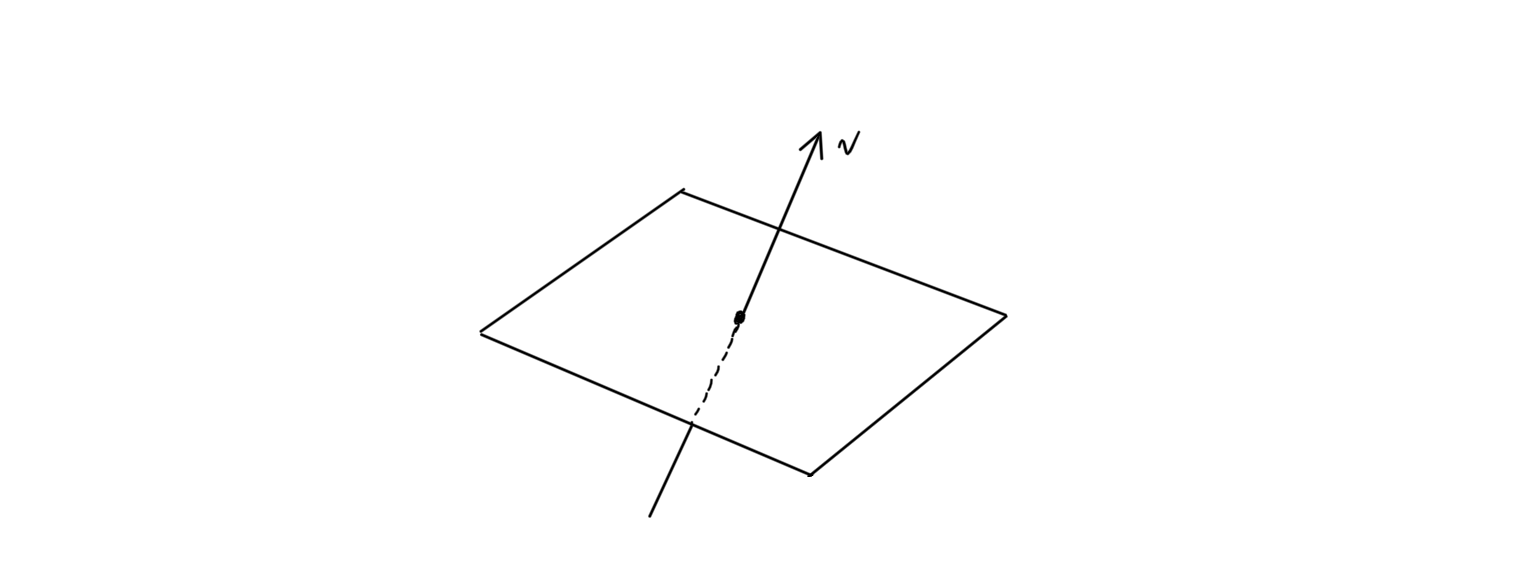
\includegraphics[scale=0.25]{Images/Rotation_Map_Eigendecomposition.PNG}
\end{center}
\end{example}

\begin{definition}
A matrix is \textit{diagonalizable} if we can perform a change of basis on it to create a diagonal matrix. 
\end{definition}

\begin{theorem}
A matrix is diagonalizable if and only if its algebraic multiplicities is equal to its geometric multiplicities. That is, if the matrix only has genuine eigenvectors. This is also equivalent to saying that all of $A$'s eigenspaces have dimension $1$. 
\end{theorem}

It is clear that since eigendecompositions are intrinsic to linear mappings, the JNF of similar matrices are the same. That is, the eigenvalues and the dimensions of the eigenspaces are invariant under a change of basis. 

\begin{proposition}
Two matrices are similar if and only if their eigendecompositions are the same. That is, if they have the same eigenvalues and the dimensions of the corresponding eigenspaces are the same. 
\end{proposition}

\begin{proof}
$(\rightarrow)$ $A \sim B \implies A = S^{-1} B S = S^{-1} P^{-1} J P S = (PS)^{-1} J (PS) \implies$ JNF of $A$ and $B$ are the same.  \\
$(\leftarrow)$ $A$ and $B$ have same JNF $\implies A = P^{-1} J P, B = Q^{-1} J Q \implies J = Q B Q^{-1} \implies A = P^{-1} Q B Q^{-1} P = (Q^{-1} P)^{-1} B (Q^{-1} P) \implies A \sim B$. 
\end{proof}

\begin{theorem}
$A \sim A^T$. 
\end{theorem}
\begin{proof}
By the proposition above, it is sufficient to prove that $A$ and $A^T$ have the same eigendecomposition. Since $(A - \lambda I)^T = A^T - \lambda I$, $\det{(A - \lambda I)} = 0 \iff \det{(A - \lambda I)^T} = \det{(A^T - \lambda I)} \implies $ $A$ and $A^T$ have the same eigenvalues. Similarly, $\big( (A - \lambda I)^d \big)^T = (A^T - \lambda I)^d \implies$ the eigenspaces of $A$ and $A^T$ have the same dimension. 
\end{proof}

\section{Further Properties of Linear Mappings}
\subsection{Adjoint Operators}
\begin{definition}
Let $A: U \longrightarrow V$ be a linear mapping between inner product spaces, with the inner product in $U$ and $V$ denoted $(\cdot,\cdot)_U$ and $(\cdot,\cdot)_V$, respectively. We can fix any $v \in V$ and define the linear function $l \in U^*$
\begin{equation}
    l(\cdot) = \big(A(\cdot), v\big)_V
\end{equation}
Since $U$ is naturally isomorphic to $U^*$, we can define
\begin{equation}
    l(\cdot) \equiv (\cdot, u^\prime)
\end{equation} 
to get 
\begin{equation}
    \big(\cdot, u^\prime \big)_U \equiv \big(A(\cdot), v \big)_V
\end{equation}
By combining $(8)$, which defines an isomorphism between $U^*$ and $V$, and $(9)$, the natural isomorphism between $U$ and $U^*$, equation $(10)$ takes the composition of these to define an isomorphism from $V$ to $U$. This isomorphism is called the \textit{adjoint} of $A$. 
\[A^\dagger: V \longrightarrow U, \;  \big(\; \cdot \;, A^\dagger v \big)_U = \big( A(\cdot), v \,\big)_V \]
By definition, given any $v \in V$, $A^\dagger v$ is defined so that the equality
\[(u, A^\dagger v) = (A u, v)\]
holds for all values of $u \in U$. 
\end{definition}

It is important to note that the adjoint is not the same as the transpose since the transpose is a mapping between the dual spaces. Furthermore, the transpose is canonically defined upon defining the linear transformation $A: U \longrightarrow V$, while defining the adjoint requires the additional structure of an isomorphism from $U$ to $U^*$ and from $V$ to $V^*$. There are two ways to define these isomorphisms. \\

First, we can define dot products on both $U$ and $V$ and define the natural isomorphism 
\begin{align*}
    &i: U \longrightarrow U^*, \; i(u) \equiv (u, \cdot) \in U^*\\
    &j: V \longrightarrow V^*, \; j(v) \equiv (v, \cdot) \in V^*
\end{align*}
This canonically creates the mapping 
\[i^{-1} A^T j: V \longrightarrow U\]
which we define as the adjoint $A^\dagger$. This method using natural isomorphisms is precisely how we have defined the adjoint above. \\

There is a second way, however. We can fix \textit{orthonomal} bases on $U$ and $V$ and then assign them their respective dual spaces (satisfying the Kronecker delta function). Let the basis of $U$ be $\{u_1, ..., u_n\}$, $U^*$ be $\{u_1^\prime, ..., u_n^\prime\}$, $V$ be $\{v_1, ..., v_m\}$, and $V^*$ be $\{v_1^\prime, ..., v_m^\prime\}$. Now we can define the isomorphisms 
\begin{align*}
    & i^\prime: U \longrightarrow U^*, \; i^\prime (u) \equiv c_1 u_1^\prime + ... + c_n u_n^\prime \\
    & j^\prime: V \longrightarrow V^*, \; j^\prime (v) \equiv k_1 v_1^\prime + ... + k_m v_m^\prime
\end{align*}
and then define the adjoint as 
\[A^\dagger \equiv i^{\prime -1} A^T j^\prime\]
Let us compare these two definitions. Given a vector $u = a_1 u_1 + ... + a_n u_n, \Tilde{u} = b_1 u_1 + ... b_n u_n \in U$, 
\begin{align*}
    &i(u)(\Tilde{u}) \equiv (u, \Tilde{u}) = \Big(\sum_{\alpha = 1}^n a_\alpha u_\alpha, \sum_{\beta = 1}^n b_\beta u_\beta \Big) = \sum_{\alpha, \beta} a_\alpha b_\beta \delta^\alpha_\beta = \sum_{\gamma=1}^n a_\gamma b_\gamma \\
    &i^\prime(u)(\Tilde{u}) \equiv \Big(\sum_{i=1}^n a_i u_i^\prime \Big) \Big( \sum_{j=1}^n b_j u_j \Big) = \sum_{i, j} a_i b_j u_i^\prime (u_j) = \sum_{i, j} a_i b_j \delta^i_j = \sum_{k=1}^n a_k b_k
\end{align*}
Similarly for vector $v = g_1 v_1 + ... g_n v_n, \Tilde{v} = h_1 v_1 + ... + h_n v_n \in V$, 
\begin{align*}
    &i(v)(\Tilde{v}) \equiv (v, \Tilde{v}) = \Big(\sum_{\alpha = 1}^n g_\alpha v_\alpha, \sum_{\beta = 1}^n h_\beta v_\beta \Big) = \sum_{\alpha, \beta} g_\alpha h_\beta \delta^\alpha_\beta = \sum_{\gamma=1}^n g_\gamma h_\gamma \\
    &i^\prime(v)(\Tilde{v}) \equiv \Big(\sum_{i=1}^n g_i u_i^\prime \Big) \Big( \sum_{j=1}^n h_j v_j \Big) = \sum_{i, j} g_i h_j v_i^\prime (v_j) = \sum_{i, j} g_i h_j \delta^i_j = \sum_{k=1}^n g_k h_k
\end{align*}
Therefore, $i = i^\prime$ and $j = j^\prime$, meaning that the two derivations of the adjoint $A = i^{-1} A^T j = i^{-1 \prime} A^T j^\prime$ are exactly the same! We must note that the basis endowed on both $U$ and $V$ must be orthonormal for it to "mimic" the inner product. The derivation of the adjoint in these two equivalent methods may help the reader further understand that the adjoint $A^\dagger$ is really just a composition of fundamental linear functions $j: V \longrightarrow V^*$, $A^T: V^* \longrightarrow U^*$, and $i^{-1}: U^* \longrightarrow U$ that are all canonically created as soon as $A: U \longrightarrow V$ is created, along with the inner product spaces $U$ and $V$. 
\[
  \begin{tikzcd}
    U \arrow{r}{A} \arrow{d}{i} & V \arrow{d}{j}\\
    U^* & V^* \arrow{l}{A^T}
  \end{tikzcd}
\]

However, it is hard to grasp a visual intuition of adjoint operators in general. Note that the properties of the transpose indicate that given $A: \mathbb{R}^n \longrightarrow \mathbb{R}^m$ with the standard orthonormal basis and dot product, the matrix representation of $A^\dagger$ is just $A^T$. If $A$ is a matrix over $\mathbb{C}$, then $A^\dagger$ is $A^H \equiv \bar{A}^T$, the \textit{Hermitian transpose}, or \textit{conjugate transpose}, of $A$. 

\begin{remark}
Note that this definition of the adjoint of linear operators is completely unrelated to the definition of an adjoint of a matrix! 
\end{remark}

We now describe one common application of adjoints. 
\begin{theorem}
Let $A \in$ Mat$(m \times n, \mathbb{R})$ with $m > n$. This means that the system of equations $A x = p$ is an overdetermined system and will have no solutions with probability 1. However, we can find the \textit{best-fit solution} of the system. That is, the vector $x$ that minimizes $||A x -p||^2$ is the solution $z$ of 
\[ A^\dagger A z = A^\dagger p\]
$z$ is therefore, the "closest approximation" of the solution of $A x = p$ that lives in $\mathbb{R}^n$. 
\end{theorem}

The QR decomposition is often used to simplify these linear least squares problems into a more manageable equation. 

\begin{theorem}[QR Decomposition]
Any real $m \times n$ matrix $A$ mapping $\mathbb{R}^n \longrightarrow \mathbb{R}^m$ may be decomposed as
\[A = Q R\] 
where $Q$ is a $m \times n$ matrix with column vectors that are pairwise orthonormal and $R$ is an upper triangular square matrix. $Q$ having pairwise orthonormal columns $\implies Q^T Q = I$, so we can simplify the normal equation
\begin{align*}
    A^T A x = A^T b & \implies (Q R)^T (Q R) x = R^T Q^T Q R x = R^T R x = R^T Q^T b \\
    & \implies R x = Q^T b \\
    & \implies x = R^{-1} Q^T b
\end{align*}
\end{theorem}

\begin{theorem}
Let $P_Y$ be the orthogonal projection onto $Y$. Then, 
\begin{enumerate}
    \item $P_Y = P_Y^2$. 
    \item $P_Y = P_Y^\dagger$. 
\end{enumerate}
\end{theorem}

\begin{theorem}[Properties of the Adjoint] Let $A, B: X \longrightarrow U, \; C: U \longrightarrow V$ be linear mappings. Then, 
\begin{enumerate}
    \item $(A + B)^\dagger = A^\dagger + B^\dagger$
    \item $(C A)^\dagger = A^\dagger C^\dagger$
    \item $(A^{-1})^\dagger = (A^\dagger)^{-1}$ if $A$ is bijective
    \item $(A^\dagger)^\dagger = A$
\end{enumerate}
\end{theorem}

\begin{definition}
Linear mapping $A$ is \textit{self adjoint} if and only if $A = A^\dagger$. If $M$ is any linear mapping, then its self-adjoint part is 
\[M_\delta = \frac{M + M^\dagger}{2}\]
\end{definition}

\begin{theorem}[Spectral Theorem]
A $n$-dimensional self-adjoint map $H$ over $\mathbb{C}$ has real eigenvalues and an orthonormal basis of genuine eigenvectors. That is, its eigendecomposition consists of $n$ pairwise orthogonal eigenspaces. 
\end{theorem}

\begin{corollary}
Given a real self-adjoint matrix $H$, there exists a real invertible matrix $M$ such that $M^\dagger H M = D$, with $D$ diagonal and the column vectors form an orthonormal basis.
\\

So, given self-adjoint $H: X \longrightarrow X$, the whole space can be written as the direct sum of pairwise orthogonal eigenspaces. 
\[X = \bigoplus_{i=1}^n E(\lambda_i)\]
which implies that every $x \in X$ can be written uniquely as 
\[x = x_1 + x_2 + ... + x_n, \; x_i \in E(\lambda_i) \]
\end{corollary}

\begin{definition}
Given that $P_j$ is the orthogonal projection onto the $j$th eigenspace $E(\lambda_j)$, that is
\[P_j (x) = x_j \in E(\lambda_j), \; \text{ ($P_j$ also self adjoint)}\]
the \textit{spectral resolution} of self-adjoint mapping $H$ is the decomposition into the form 
\[H = \sum_j \lambda_j P_j \implies H x = \bigg( \sum_j \lambda_j P_j \bigg) x = \sum_j \lambda_j x_j\]
The resolution of the identity is
\[I = \sum_j P_j\]
\end{definition}

\begin{proposition}
Given the spectral resolution of self-adjoint $H$, 
\[H  = \sum_j \lambda_j P_j \implies H^2 = \sum_j \lambda_j^2 P_j\]
\end{proposition}

Note that the spectral resolution of a self adjoint mapping is precisely the eigendecomposition of the mapping into its 1-dimensional eigenspaces. It is merely a simpler form of the eigendecomposition in the specific case when the linear mapping is self-adjoint. 

\begin{theorem}
Let $H, K$ be self-adjoint mappings such that $H K = K H$. Then $H$ and $K$ have the same spectral resolution, i.e. they have the same eigendecomposition. 
\[H = \sum_j a_j P_j, \; \; K = \sum_j b_j P_j\]
\end{theorem}
\begin{proof}
$ x \in E(a) H x = a x \implies K H x = a K x \implies H K x = a K x \implies K x \in E(a)$. Similarly, we can do this with $K$ to find $x \in E(a) \implies H x \in E(a)$, meaning that $K$ and $H$ have the same eigendecompositions (though their eigenvalues are not necessarily equal). 
\end{proof}

\begin{definition}
Map $A$ is \textit{anti-self adjoint }if $A^\dagger = - A$. Conjugate symmetry implies that
\[ A^\dagger = A \iff (i A)^\dagger = - (i A)\]
So, given an anti-self adjoint map $A$, we can apply the spectral resolution to $iA$. 
\end{definition}

\begin{theorem}
Given anti-self adjoint $A: \mathbb{C}^n \longrightarrow \mathbb{C}^n$, 

i) eigenvalues of $A$ are purely imaginary

ii) we can choose an orthonormal basis of eigenvectors of $A$
\end{theorem}

\begin{proof}
This easily follows from the Spectral Theorem. 
\end{proof}

\begin{definition}
$N: X \longrightarrow X$ is a \textit{normal mapping} if $N^\dagger N = N N^\dagger$. Self-adjoint, anti-self adjoint, and unitary matrices are all normal. Surprisingly, the set of normal matrices are not closed under addition nor multiplication, so they do not form a group. 
\end{definition}

\begin{theorem}
A map $N$ is normal if and only if it has an orthonormal basis of eigenvectors, i.e. it is unitarily diagonalizable. That is, 
\[N = U^\dagger D U \]
\end{theorem}

\begin{proof}
$(\rightarrow)$ Let 
\[H = \frac{1}{2} (N + N^\dagger), \; A = \frac{1}{2} (N - N^\dagger)\]
$N^\dagger N = N N^\dagger \implies A H = H A$, where $H$ is self adjoint, $A$ is anti-self adjoint, and $N = H + A, N^\dagger = H - A$. Since $A H = H A$, they have the same spectral resolution of orthonormal eigenspaces, which also forms the same spectral resolution for $N = H + A$. \\
$(\leftarrow)$ $A = U^\dagger D U \implies A^\dagger A = (U^\dagger D U) (U^\dagger \bar{D} U) = U^\dagger D \bar{D} U = A A^\dagger$. 
\end{proof}

\subsection{Lie Groups and the Exponential Map}
\begin{definition}
Aut$(V)$ of vector space $V$ also forms a group under composition. We denote it GL$(V)$. The group of automorphisms of $\mathbb{R}^n$ and $\mathbb{C}^n$ is denoted GL$(\mathbb{R}^n)$ and GL$(\mathbb{C}^n)$, respectively. The group of all invertible $n \times n$ matrices over $\mathbb{R}$ and $\mathbb{C}$ is denoted GL$_n(\mathbb{R})$ and GL$_n(\mathbb{C})$. GL$_n(\mathbb{R})$ is also denoted GL$(n, \mathbb{R})$, and similarly for GL$(n, \mathbb{C})$. 
\end{definition}

\begin{proposition}
Given that $V$ is a real vector space, 
\[GL(V) \simeq GL(\mathbb{R}^n) \simeq GL_n (\mathbb{R})\]
since GL$_n(\mathbb{R})$ are representations of linear operators. Similarly, if $V$ is a complex vector space, 
\[GL(V) \simeq GL(\mathbb{C}^n) \simeq GL_n (\mathbb{C})\]
\end{proposition}

\begin{definition}
The group of all real $n \times n$ matrices that have determinant $1$ is called the \textit{special linear group}, denoted SL$_n (\mathbb{R})$. It is a subgroup of GL$_n (\mathbb{R})$. The group of all complex $n \times n$ matrices with determinant $1$ is denoted SL$_n (\mathbb{C})$. It is a subgroup of GL$_n(\mathbb{C})$. 
\end{definition}

\begin{definition}
An \textit{isometry} $M$ of metric space $(X, d)$ is a mapping that preserves all distances. That is, for all $x, y \in X$, 
\[d(x, y) = d(M x, M y) \]
The set of all isometries, denoted Isom$(X)$, is a group that is generated by all translations, rotations, and reflections. 
\end{definition}

Since linear maps always preserve the origin, we will focus on origin-preserving isometries, which is a subgroup called the orthogonal group.

\begin{definition}
The \textit{orthogonal group} of a real Euclidean space of dimension $n$, denoted $O(n)$, is the group of all origin-preserving isometries of the space consisting of rotations and reflections. The matrix representation of this group is the set of real $n \times n$ matrices where the column vectors form an orthonormal basis. Note that the determinant of every element of $O(n)$ is $\pm 1$. 
\end{definition}

\begin{definition}
An \textit{orthogonal matrix} is the matrix representation of an element in $O(n)$. It is the real $n \times n$ matrix where all the column vectors are pairwise orthogonal and all have magnitude 1. 
\end{definition}

\begin{proposition}
The rows of an orthogonal matrix are also pairwise orthonormal.
\end{proposition}

\begin{proposition}
Given an orthogonal matrix $M$,
\[M^T = M^{-1}\]
\end{proposition}

\begin{definition}
The \textit{special orthogonal group} of a real Euclidean space of dimension $n$, denoted $SO(n)$, is the group of all isometries that preserve the handedness of the space consisting only of rotations. It is a subgroup of $O(n)$. The matrix representation of this group is the set of real $n \times n$ matrices where the column vectors are pairwise orthonormal and the determinant $=1$. 
\end{definition}

We extend this concept to complex Euclidean spaces. 

\begin{definition}
The \textit{unitary group of degree $n$} is the group of all complex $n \times n$ matrices where the columns are pairwise orthogonal. It is denoted $U(n)$. 
\end{definition}

\begin{example}
$U(1)$ is the set of complex numbers with norm $1$. 
\end{example}

\begin{definition}
The \textit{special unitary group of degree $n$} is the group of all complex $n \times n$ matrices where the columns are pairwise orthogonal and determinant $=1$. It is denoted $SU(n)$. 
\end{definition}

The groups mentioned in this section are examples of \textit{Lie Groups}. Lie groups in general will not be defined in here, since they require knowledge of smooth manifolds and differential geometry. In order to analyze these abstract groups, we use the exponential map $e \in$ End$($ Mat$(n, \mathbb{F})$ to reduce these Lie groups to Lie algebras.

\subsection{Singular Values, Norms of Linear Mappings}
Since the algebra of linear operators is itself a vector space, we can also define structures on it, too. We focus on matrix norms. 

\begin{definition}
Let $A: X \longrightarrow U$ be linear. Then, we define
\[||A|| = \sup_{||x||=1} ||A x||\]
Note that $||A x||$ is measure with respect to the norm of $U$ and $||x||$ the norm of $X$. 
\end{definition}

There is a very nice visualization of this. Given that $\dim{X}=n$, imagine the $n$-dimensional unit ball in $X$ being transformed under $A$. The image of the ball should be an ellipsoid (of dimension $\leq m$) in $U$. 
\begin{center}
    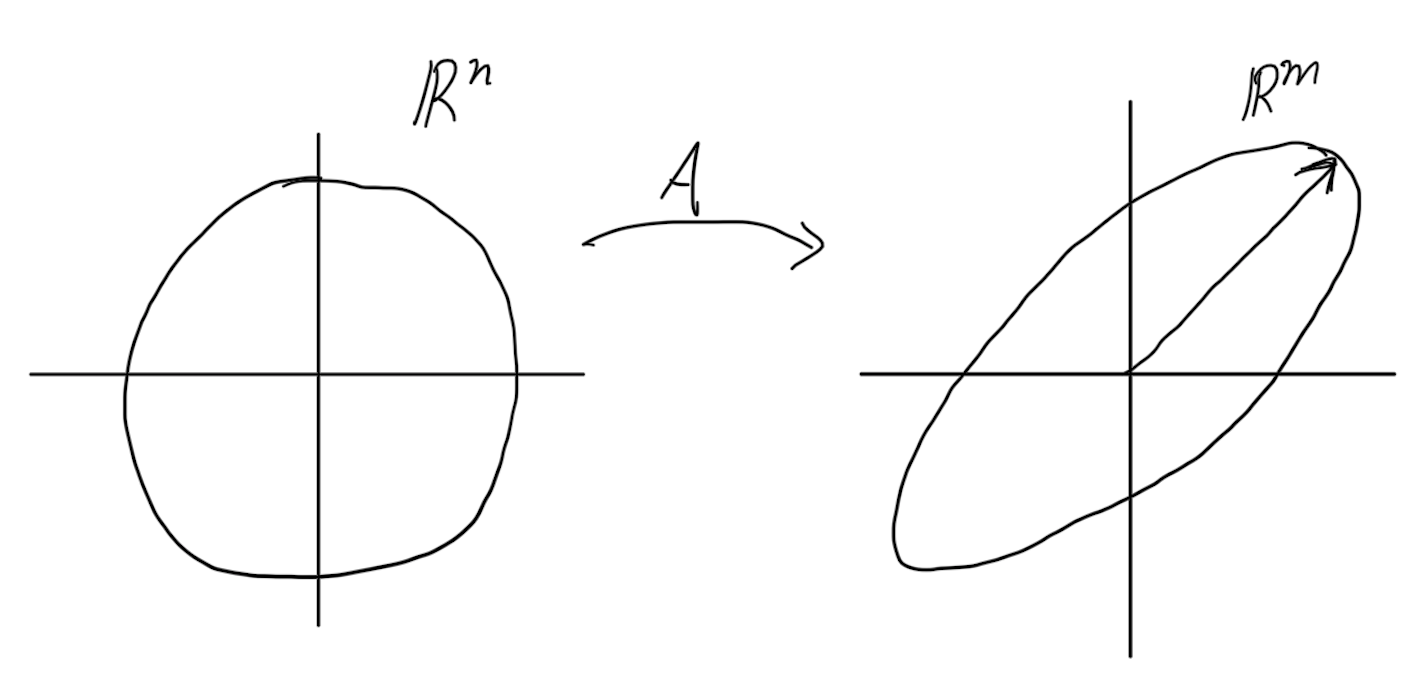
\includegraphics[scale=0.4]{Images/Matrix_Norm_Visualization.png}
\end{center}
The norm of $A$ is the length of the major axis of the ellipsoid. 

\begin{theorem}
\begin{align}
    ||A z|| \leq ||A|| ||z|| \text{ for all } z \in X \\
    ||A|| = \sup_{||x||, ||v|| = 1} (A x, v)
\end{align}
\end{theorem}
\begin{proof}
\begin{align*}
    &||A z|| \leq \sup{||A z||} = \sup{\Big|\Big| A \frac{z}{||z||} \Big|\Big|} = ||A|| ||z|| \\
    &||u|| \equiv \max_{||v||=1} (u, v) \implies ||A x|| \equiv \max_{||v||=1} (Ax, v) \implies ||A|| \equiv \sup_{||x||, ||v|| =1} (A x, v)
\end{align*}
\end{proof}

\begin{theorem}[Properties of Matrix Norm]
Let there exist any $k \in \mathbb{F}$, with any $A, B: X \longrightarrow U$, $C: U \longrightarrow V$. Then, 
\begin{enumerate}
    \item $||k A|| = |k| ||A||$
    \item $||A + B|| \leq ||A|| + ||B||$
    \item $||C A|| \leq ||C|| ||A||$
    \item $||A|| = ||A^\dagger||$
\end{enumerate}
\end{theorem}

\begin{definition}
The \textit{spectral radius} of $A$ is defined
\[r(A) \equiv \max_i |a_i|, \; a_i \text{ are eigenvalues}\]
\end{definition}

\begin{proposition}
A simple lower and upper bound of $||A||$ can be defined
\[ r(A) \leq ||A|| \leq \bigg( \sum_{i, j} a_{i j}^2 \bigg)^\frac{1}{2}\]
\end{proposition}

Matrix norms have extremely useful applications in determining the existence of invereses. 

\begin{theorem}
Let $A$ be invertible and 
\[||A - B|| < \frac{1}{||A^{-1}||}\]
in the sense that $B$ is "close" to $A$. Then $B$ is invertible. 
\end{theorem}
We now proceed to another crucial decomposition, called the singular value decomposition. While the JNF allows us to choose the most convenient choice of basis for a square matrix, the Singular Value Decomposition (SVD) allows us to decompose general $m \times n$ matrices. 

\begin{theorem}[Singular Value Decomposition]
Any linear mapping $M$ from an $n$-dimensional inner product space to a $m$-dimensional inner product space can be decomposed into 
\[ M = U \Sigma V^\dagger = \begin{pmatrix}
 \vert & \vert & \vert & \vert\\
y_1 & y_2 & \ldots & y_m \\
\vert & \vert & \vert & \vert
\end{pmatrix}\begin{pmatrix}
\sigma_1 & & & &0\\
&\ddots &&& \vdots \\
& & \sigma_p & & 0\\
& & & \ddots &\vdots \\
0 & \ldots &0& \ldots &0
\end{pmatrix} \begin{pmatrix}
\text{---}&x_1&\text{---} \\
\text{---}&x_2&\text{---} \\
\text{---}&\vdots&\text{---} \\
\text{---}&x_n&\text{---}
\end{pmatrix} \]
where $U \in U(m), V \in U(n)$ and $\Sigma$ has diagonal elements with nonnegative real entries. Also, $p = $ rank$(M) \leq \min{\{n,m\}}$. This form is known as the \textit{singular value decomposition}. The columns of $U$, denoted $y_i$, are called the \textit{left singular vectors} and the columns of $V$ (i.e. the rows of $V^\dagger$), denoted $x_i$, are called the \textit{right singular vectors}. The diagonal entries of $\Sigma$ are called the \textit{singular values}. 
\\

The SVD is unique up to the order of singular values, but it is generally constructed so that $\sigma_1 \geq \sigma_2 \geq ... \geq \sigma_p$. 
\end{theorem}

To provide a brief, yet unrigorous, justificiation of why the SVD exists, we look at the linear mapping $M: X \longrightarrow Y$, with $\dim{X} = n, \dim{Y} = m$. If $M$ is injective $(\iff m \geq n)$, given the basis $\{e_i\}$ for $X$, we can complete the linearly independent set $\{Me_i\}_{i=1}^n$ to a basis in $Y$ and represent $M$ as the mapping
\[\Sigma_{inj} = \begin{pmatrix}
&&\\
&I_n&\\
&&\\
0&\ldots &0
\end{pmatrix}\]
If $M$ is surjective $(\iff m \leq n)$, then given basis $\{f_i\}_{i=1}^m$ of $Y$, we can choose a basis $\{e_j\}_{j=1}^n$ of $X$ such that $M(e_i) = f_i (i = 1, 2, ..., m)$, and $M(e_i) = 0$ when $i > m$. This produces the matrix
\[\Sigma_{surj} = \begin{pmatrix}
&&&0\\&I_m&& \vdots \\&&&0\end{pmatrix}\]
We now present the following theorem without proof. 

\begin{theorem}
Any map $M: X \longrightarrow Y$ can be written as a surjective map followed by an injective map. 
\end{theorem}

This theorem implies that any map, when given the right choice of basis, can be written as 
\[ \Sigma_{inj} \Sigma_{surj} = \begin{pmatrix}
&&&...&0\\
&I_p&&...&0\\
&&&...&...\\
...&...&...&...&0\\
0&0&...&0&0
\end{pmatrix} = \begin{pmatrix}
1&&&&0\\
&...&&&...\\
&&1&&0\\
&&&...&...\\
0&...&0&...&0
\end{pmatrix}\]
where rk$(M) = p = $ the number of $1$'s in $\Sigma_{inj} \Sigma_{surj}$. As for choosing the proper set basis for $X$ and $Y$, we can find these passive transformations in the unitary groups $U(n)$ and $U(m)$. 
\\

We now present a geometric description of the singular value decomposition. Think of the unit $n$-ball being rotated and flipped ($V^\dagger$ applied) under the unitary transformation. Then, it is stretched along its othogonal axes to result in an ellipsoid living in an $m$-dimensional space. The factor of stretching and compressing the axes are precisely the singular values. Finally, this ellipsoid is rotated and flipped ($U$ applied) back to its original basis. 

\begin{theorem}
Geometrically, we can see that the largest singular value is the matrix norm, also called the operator norm. 
\[||M|| = \sigma_1\]
\end{theorem}

\begin{theorem}[Properties of Singular Values] Given linear mapping $A$ from a $n$-dimensional inner product space to $m$-dimensional inner product space, 
\begin{enumerate}
    \item $\sigma_i(A) = \sigma_i (A^T) = \sigma_i (A^\dagger) = \sigma_i (\bar{A})$
    \item $\forall \; U \in U(m), V \in U(n), \; \sigma_i (A) = \sigma_i (U A V)$
    \item Relation to eigenvalues
\[\sigma_i^2(A) = \lambda_i (A^\dagger A) = \lambda_i (A A^\dagger)\]
\end{enumerate}
\end{theorem}

We now present the (not the best) process of computing SVD of small matrices by hand. Given matrix $M$, $M = U \Sigma V^\dagger \implies M^\dagger M = V \Sigma^2 V^\dagger$. The eigenvalues of $M^\dagger M$ are $\sigma_i^2$ with corresponding eigenvectors being the columns of $V$, which can all be found by putting $M^\dagger M$ into JNF. We repeat this process for $M M^\dagger = U \Sigma^2 U^\dagger$ to find the eigenvectors that make up the column vectors of $U$. 

\begin{theorem}
Let $A: X \longrightarrow Y$, with $\dim{X} = n, \dim{Y} = m$, and let $k \leq \min{\{m, n\}}$, with $A = U \Sigma V^\dagger$. Then, amongst all rank $k$ $m \times n$ matrices $B$, the matrix $A^{(k)}$ minimizes 
\[||A-B||_2, \; A^{(k)} = U \Sigma^{(k)} V^\dagger\]
and $\Sigma^{(k)}$ is $\Sigma$ with $\sigma_{k+1} = \sigma_{k+2} = ... = 0$. Therefore, to see how "close" $B$ is to $A$, we can compare the singular values of $A$ and $B$, given that they both have the same unitary matrices $U$ and $V$. 
\end{theorem}

The singular value decomposition has many applications in high dimensional data analysis and data compression. For example, in a set of $m$ data points in $\mathbb{R}^n$ that each lie in the rows of matrix $A$, if the singular values of $A$ suddenly drops (e.g. 120, 118, 107, 98, 2, 1, 0.3, ...) then we can determine that the points "almost" lie in a subspace in $\mathbb{R}^n$. Knowing this allows us to compress high dimensional data to $A^{(k)}$, which is a more manageable form. This is especially useful in the data compression of electronic images, where each pixel is treated as a single number to form a matrix. 

It can also be used to define the "pseudo-inverse" of a matrix that may not be invertible. 

\begin{definition}
Given matrix $M = U \Sigma V^\dagger$ in SVD, we define the \textit{pseudo-inverse} $M^+ = V \Sigma^+ U^\dagger$, where $\Sigma^+$ is $\Sigma$ with entries $\sigma_i^{-1}$, or $0$ if $\sigma_i = 0$. For example,
\[ \Sigma = \begin{pmatrix}3&0&0\\0&2&0\\0&0&0\end{pmatrix} \implies \Sigma^+ = \begin{pmatrix}1/3&0&0\\0&1/2&0\\0&0&0\end{pmatrix}\]
$\implies M^+ M = V \Sigma^+ \Sigma V^\dagger$. If $M$ is square and all $\sigma_i \neq 0$, then $M^\dagger M = V V^\dagger \implies M^\dagger M = I \implies  M^+ = M^{-1}$. 
\end{definition}

By computing the SVD of $M$, where $\sigma_p \neq 0, p =$ rk$\,M = $ rk$\,\Sigma$, we can automatically compute the 4 fundamental spaces. 
\[M = U \Sigma V^\dagger = \begin{pmatrix}&&&&|&\\&&&&|&\\&&U&&|&U^\prime\\&&&&|&\\&&&&|&
\end{pmatrix} \begin{pmatrix}
\sigma_1&&&&0\\
&\sigma_2&&&0\\
&&...&&...\\
&&&\sigma_p&0\\
0&0&...&0&0
\end{pmatrix}\begin{pmatrix}
&&&&\\&&&&\\&&V^\dagger&&\\&&&&\\\text{---}&\text{---}&\text{---}&\text{---}&\text{---}
\\&&V^{\dagger \prime}&&
\end{pmatrix}\]
\begin{enumerate}
    \item $\im{M} = C(U)$
    \item $\ker{M} = R(V^{\dagger \prime}) = C(V^\prime)$
    \item $\ker{M^\dagger} = C(U^\prime)$
    \item $\im{M^\dagger} = C(V) = R(V^\dagger)$
\end{enumerate}

One of the main differences between the JNF and SVD of a matrix $A$ lies in how they are affected by perturbations in the elements of $A$. For example, take the small change 
\[ A = \begin{pmatrix}
1 & 1\\
0 & 1
\end{pmatrix} \longrightarrow A^\prime  = \begin{pmatrix}
1 & 1 \\
0 & 1.00001
\end{pmatrix}\]
The SVD of $A^\prime$ will "change" continuously for changes in the elements of $A$, but the JNF of $A$ is completely different from the JNF of $A^\prime$. More specifically, the JNF of $A$ is $A$ itself, but the JNF os $A^\prime$ is now diagonalizable, meaning that the 2-dimensional eigenspace $E(1)$ "breaks up" into two 1-dimensional eigenspaces from small perturbations. 

\begin{definition}
The \textit{Frobenius norm} of a $m \times n$ matrix $A$ is defined
\[||A||_F \equiv \sqrt{\Tr{(A^\dagger A)}} = \sqrt{\Tr{\Sigma^2}} = \bigg( \sum_{i, j} a_{i j}^2 \bigg)^{\frac{1}{2}} \]
By Singular Value Decomposition, we can reduce its calculations to
\[ ||A||_F = \sqrt{\sum_i \sigma_i^2}\]
where $\sigma_i$'s are the singular values. Clearly, 
\[||A||_2 \leq ||M||_F\]
In quantum mechanics, the Frobenius norm is also called the \textit{Hilbert Schmidt norm} in the context of infinite dimensional Hilbert spaces. 
\end{definition}

We end by defining two more common decompositions of square matrices. 

\begin{theorem}[Schur Decomposition]
Every $n \times n$ matrix $A$ over $\mathbb{C}$ can be decomposed into
\[A = Q T Q^\dagger\]
where $Q \in U(n)$ and $T$ is upper triangular. 
\end{theorem}
\begin{proof}
This is an obvious result of the Grahm-Schmidt algorithm. 
\end{proof}

\begin{theorem}[Polar Decomposition]
Every complex $n \times n$ matrix $A$ can be factored into the form
\[A = U P\]
where $U \in U(n)$ and $P$ is a positive semidefinite self-adjoint matrix. If $A$ is a real matrix, then $U \in O(n)$. 
\end{theorem}
\begin{proof}
We take the SVD to get 
\[A = W \Sigma V^\dagger\]
and we can assign 
\[U = W V^\dagger, \; P = V \Sigma V^\dagger\]
Since $V, W$ are unitary, this confirms that $P$ is positive definite and self-adjoint along with $U$ being unitary. Thus, the existence of the SVD implies the existence of the polar decomposition. 
\end{proof}

\subsection{Positive Definite Matrices}
\begin{definition}
A self-adjoint linear mapping $H$ from a real or complex Euclidean space onto itself is \textit{positive definite} if 
\[(x, H x) > 0 \text{ for all } x \neq 0\]
$H$ is called \textit{positive semidefinite} if 
\[(x, H x) \geq 0\]
\end{definition}

\begin{theorem}[Polar Decomposition]
Given a Euclidean space $\mathbb{E}^n$ and any linear endomorphism $f$ of $\mathbb{E}^n$, there are two positive definite self-adjoint linear maps $h_1, h_2 \in$ End$(\mathbb{E}^n)$ and $g \in$ O$(n)$ such that
\[f = g \circ h_1 = h_2 \circ g\]
That is, such that $f$ can be decomposed into the following as shown in this commutative diagram. 
\[\begin{tikzcd}
\mathbb{E}^n \arrow{r}{h_2} & \mathbb{E}^n \\
\mathbb{E}^n \arrow{u}{g} \arrow{ur}{f} \arrow{r}{h_1} & \mathbb{E}^n \arrow{u}{g}
\end{tikzcd}\]
\end{theorem}

\begin{theorem}[Properties of Positive Definite Matrices] Here we state basic properties. 
\begin{enumerate}
    \item $I$ is positive definite. 
    \item Positive mappings form a subspace in the space of linear mappings. 
\begin{align*}
    &M, N \text{ positive} \implies M + N \text{ is positive} \\
    &M \text{ positive} \implies a M \text{ is positive for all} a \in \mathbb{F}
\end{align*}
    \item $H$ positive and $Q$ invertible $\implies Q^\dagger H Q$ positive. 
\end{enumerate}
\end{theorem}

\begin{theorem}
$H$ is positive definite if and only if all of its eigenvalues are positive. Furthermore, every positive mapping is invertible.
\end{theorem}

\begin{theorem}
Every positive mapping $M$ has a unique positive square root. That is, there exists a unique positive mapping $N$ such that
\[ N^2 = M \]
We denote $N$ as $\sqrt{M}$. 
\end{theorem}

\begin{definition}
Given that $M, N$ are positive definite mappings. 
\[M > N \iff M - N > 0, \text{ that is, $M$ is positive}\]
\end{definition}

\begin{theorem}
If $M, N$ are positive definite mappings 
\[ M > N \implies M^{-1} < N^{-1}\]
\end{theorem}

\begin{proposition}
In $\mathbb{R}^n$ endowed with the dot product, a $n \times n$ matrix $A$ is positive definite if and only if 
\[(x, A y) = x^T A y > 0 \]
for every $x, y \in \mathbb{R}^n$. $A$ is positive semi-definite if and only if 
\[(x, A y) = x^T A y \geq 0\]
\end{proposition}

The following is a useful fact regarding inner products of $\mathbb{R}^n$. 
\begin{proposition}
The set of all inner products that can be defined on $\mathbb{R}^n$ is bijective to the set of positive-definite symmetric $n \times n$ matrices $A$ (which is itself bijective to the set of all positive-definite mappings). That is, every inner product of $\mathbb{R}^n$ can be defined 
\[(x, y) \equiv x^T A y\]a
Note that when $A = I_n$, the inner product is the regular dot product.
\end{proposition}

\subsection{Stochastic Matrices, Markov Chains}
\begin{definition}
A real $n \times n$ matrix $P$ is \textit{entrywise positive} if all entries are positive real numbers. We similarly define entrywise positive vectors having components as positive real numbers. With this notion of positiveness. We can define
\[A > B \iff A - B > 0 \iff (A-B)_{i j} > 0 \; \forall i, j\]
\end{definition}

\begin{remark}
Note that this definition of positive matrices is \textit{not} the same as positive-definite matrices! 
\end{remark}

\begin{theorem}[Perron's Theorem]
Every entrywise positive matrix $P$ has a real \textit{dominant eigenvalue}, denoted $\lambda(P) \in \mathbb{R}$ satisfying
\begin{enumerate}
    \item $\lambda(P) > 0$, and the associated eigenvector $h >0$
    \item $\lambda(P)$ is a simple eigenvalue
    \item every other eigenvalue $\kappa$ satisfies: $|\kappa| < \lambda(P)$
    \item there is no other eigenvector $\geq 0$, i.e. all other eigenvectors have at least 1 negative entry.
\end{enumerate}
\end{theorem}

\begin{definition}
A \textit{stochastic matrix} is a matrix $A$ where the elements of each column $a_i$ sum up to $1$. $A$ is \textit{doubly stochastic} if $A$ and $A^T$ are stochastic. 
\end{definition}

\begin{theorem}
Let $S > 0$ be a positive stochastic matrix. Then, $\lambda(S) = 1$. Furthermore, given any nonnegative vector $x \geq 0$, 
\[\lim_{N \rightarrow \infty} S^N x = c h\]
where $h$ is the dominant eigenvector and $c$ is some positive constant. 
\end{theorem}

A common application of this theorem likes in probability and statistics. Since nonnegative stochastic matrices can be used to represent discrete-time Markov Chains, with the dominant eigenvector representing the stationary distribution $\pi$. 

Another application lies within defining Google's Page Rank Algorithm. Upon representing a page as a node, if there is one link that directs the user from page $A$ to page $B$, we can represent this as an oriented path from node $A$ to node $B$. Given that we have $n$ nodes, we can construct a $n \times n$ matrix $A$ where 
\[a_{i j} \equiv  \frac{\text{number of paths from node $i$ to node $j$}}{\text{number of nonzero entries in $j$th column}}\]

For example, the adjacency matrix of the directed graph of five nodes 
\begin{center}
    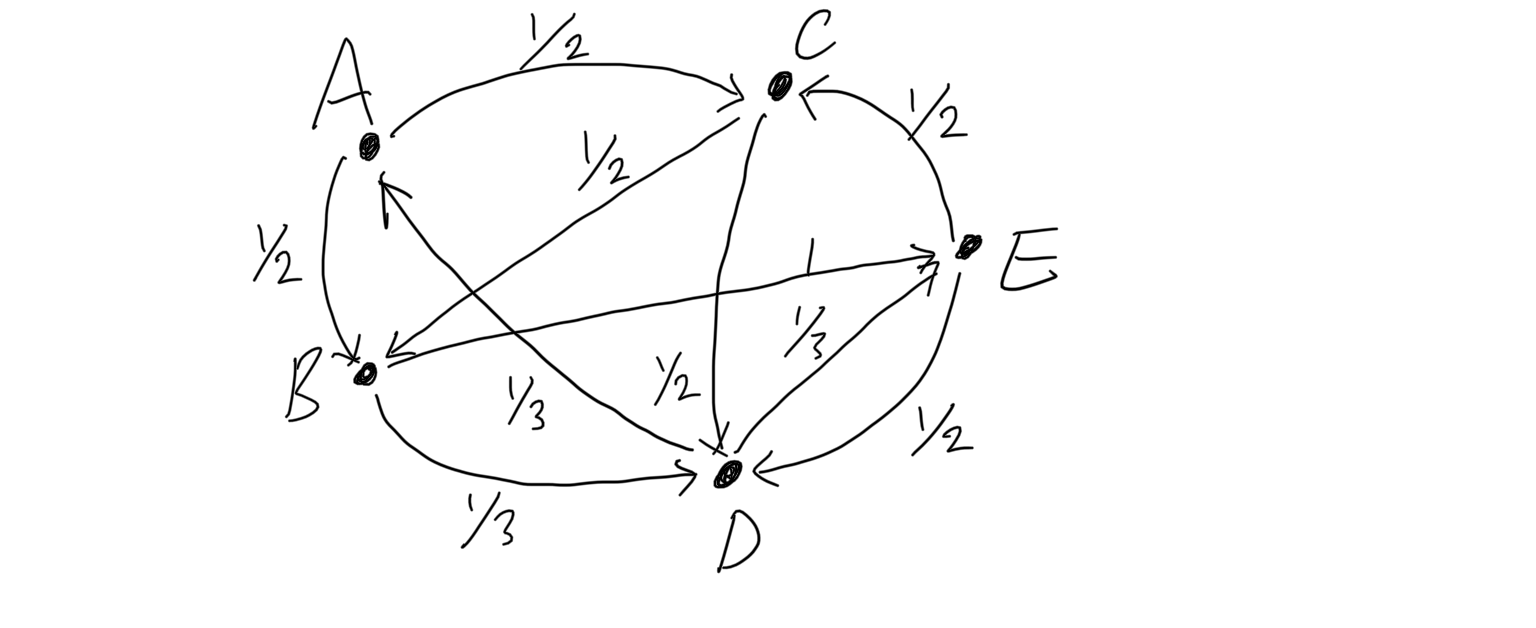
\includegraphics[scale=0.22]{Images/Markov_Chain_Example.PNG}
\end{center}
is
\[\begin{pmatrix}0&0&0&\frac{1}{3}&0\\
\frac{1}{2}&0&\frac{1}{2}&\frac{1}{3}&0\\
\frac{1}{2}&0&0&0&\frac{1}{2}\\
0&0&\frac{1}{2}&0&\frac{1}{2}\\
0&1&0&\frac{1}{3}&0\end{pmatrix}\]
However, the theorem above requires the matrix to be strictly positive, which is often not true for Markov chains in general. This theorem does not hold true in the following example, 
\[A = \begin{pmatrix}
0&0&0&\frac{1}{3} \\
\frac{1}{2}&0&0&\frac{1}{3} \\
0&0&0&\frac{1}{3} \\
\frac{1}{2}&0&0&0
\end{pmatrix} \implies A^{1000} 
    \begin{pmatrix}
\frac{1}{4} \\ \frac{1}{4} \\ \frac{1}{4} \\ \frac{1}{4}
\end{pmatrix} = 
    \begin{pmatrix}
0 \\ 9/20 \\ 11/20 \\ 0
\end{pmatrix}, \; A^{1001} 
    \begin{pmatrix}
\frac{1}{4} \\ \frac{1}{4} \\\frac{1}{4} \\ \frac{1}{4}
\end{pmatrix} = 
    \begin{pmatrix}
0 \\ 11/20 \\ 9/20 \\ 0
\end{pmatrix}
\]
That is, $A^N v$ oscillates between these two values. Furthermore, given three notes $A, B, C$ as such
\begin{center}
    
\includegraphics[scale=0.25]{Images/Degeneratre_Markov_Chain.PNG} 
\end{center}
the entries of the adjacency matrix is not well-defined. 
\[ \begin{pmatrix} 0&0&? \\0&0&? \\1&1&?\end{pmatrix}\]
Google CEO Larry Page actually developed a solution by implementing what he called a \textit{dampening factor}. Given stochastic matrix $B_{i j} = \frac{1}{N}$, he redefined the chain to be 
\[M = \alpha A + (1-\alpha) B, \; 0< \alpha < 1\]
It is clear that $M$ is now a strictly positive stochastic matrix. The $\alpha$ is the dampening factor, and its optimal value is known to be about $0.67$. The value of the alpha determines how much of the data is "washed away." When $\alpha = 0$, none of the data is lost, and when $\alpha = 1$, all of the data is lost. 

Due to the limitations of Perron's theorem, we can extend it with the following.

\begin{theorem}[Frobenius Extension to Perron]
Any $n \times n$ matrix $F \geq 0$, $F \neq 0$ has eigenvalue $\lambda$ such that
\begin{enumerate}
    \item $\lambda \geq 0$ and $F h = \lambda h$, $h\geq 0$ \item every eigenvalue $\kappa$ satisfies: $|\kappa| \leq \lambda$ 
    \item if $|\kappa| = \lambda$, then 
\[\kappa = e^{\frac{2 \pi i k}{m}} \lambda, \; k, m \in \mathbb{Z}_+, \; m \leq n\]
\end{enumerate}
\end{theorem}

\subsection{Duality Theorem}
In this section we will denote vector inequalities as entry-wise inequalities.Recall that elements of a vector space $X$ can be interpreted as column vectors, and elements of the dual of the vector space $X^*$ can be interpreted as row vectors. Therefore, value of $\phi$ at $x$ is denoted
\[\phi (x) = \phi_1 x_1 + \phi_2 x_2 + ... + \phi_n x_n\]
Furthermore, the dual of $X^*$ is $X$ itself, and given that $Y$ is a linear subspace of $X$, the annihilator of $Y^\perp$ is $Y$. 
\[X = X^{**}, \;\; Y = Y^{\perp\perp}\]
Suppose $Y$ is defined as the linear space spanned by the $m$ vectors $y_1, y_2, ..., y_m$ in $X$. That is, $Y$ consists of all vectors $y$ of the form
\[y = \sum_{j=1}^m a_j y_j\]
It is clear by linearity that $\phi$ belongs to $Y^\perp$ if and only if
\[\phi (y_j) = 0, \;\; j = 1, 2, ..., m\]
That is, a vector $y$ can be written as a linear combination of $m$ given vectors $y_j$ if and only if every $\phi$ that annihilates the $m$ vectors a also annihilates $0$. Now, we state a theorem that allows us to check if a vector $y$ can be written as a \textit{nonnegative} linear combinations of the $y_j$s. 

\begin{theorem}
A vector $y$ can be written as a linear combination of given vectors $y_j$ with nonnegative coefficients if and only if every $\zeta \in X^*$ that satisfies 
\[ \zeta (y_j) \geq 0, \;\; j = 1, 2, ..., m\]
also satisfies 
\[\zeta (y) \geq 0\]
\end{theorem}
\begin{proof}
The proof is not the easiest to construct rigorously, but it can be visualized easily. 
\end{proof}

\begin{corollary}
Given a $n \times m$ matrix $Y$, a vector $y$ with $n$ components can be written in the form 
\[y = Y p, \;\; p \geq 0\]
if and only if every row vector $\zeta$ that satisfies 
\[\zeta Y \geq 0\]
also satisfies 
\[\zeta y \geq 0\]
\end{corollary}

\begin{theorem}
Given an $n \times m$ matrix $Y$ and a column vector $y$ with $n$ components, the inequality 
\[y \geq Y p, \;\; p \geq 0\]
is satisfied if and only if every $\zeta$ that satisfies
\[\zeta Y \geq 0, \;\; \zeta \geq 0\]
also satisfies 
\[\zeta y \geq 0\]
\end{theorem}

\begin{theorem}[Duality Theorem]
Let $Y$ be a given $n \times m$ matrix, $y$ a given column vector with $n$ components, and $\gamma$ a given row vector with $m$ components. Let 
\[S = \sup_p \{\gamma p\}\]
for all column vectors $p$ with $m$ components satisfying $y \geq Y p, \; p \geq 0$. A well-defined such $p$ is called \textit{supremum admissible}. Additionally, let 
\[s = \inf_\zeta \{ \zeta y\}\]
for all row vectors $\zeta$ with $n$ components satisfying $\gamma \leq \zeta Y, \; \zeta \geq 0$. A well-defined such $\zeta$ is called \textit{infimum admissible}. Given that admissible vectors $p$ and $\zeta$ exist, then $S$ and $s$ are finite and 
\[S = s\]
\end{theorem}

\subsection{Alternating Sign Matrices}
We now describe a generalization of permutation matrices. While these kinds of matrices haven't been studied deeply, its applications lie in measuring the computational complexity of the Dodgson Condensation method for computing matrix determinants. The set of alternating sign matrices also forms a bijection with combinatorial objects, such as plane partitions, aztec diamonds, ice models, etc. 

\begin{definition}
A matrix with elements $0, -1, 1$ where nonzero entries must alternate in the following pattern: $1, -1, 1, ..., -1, 1$ (i.e. begin and end with $1$) is called an \textit{alternating sign matrix}. This means that every row and column must add up to $1$. 
\end{definition}

\begin{example}
The following are alternating sign matrices. 
\[\begin{pmatrix}
0&1&0&0\\1&-1&0&1\\0&1&0&0\\0&0&1&0
\end{pmatrix}, \begin{pmatrix}
0&1&0\\1&-1&1\\0&1&0
\end{pmatrix}\]
\end{example}

As with permutation matrices, we would like to calculate how many $n \times n$ alternating sign matrices there are for a given $n$. Let the set of all $n \times n$ alternating sign matices be denoted
\[\text{ASM}(n)\]

\begin{proposition}[Alternating Sign Matrix Conjecture (Proved)]
The number of $n \times n$ alternating sign matrices is the following. 
\[\text{card ASM}(n) = \prod_{k=0}^{n-1} \frac{(3k+1)!}{(n+k)!}\]
\end{proposition}

We now define a bijection between ASMs and another type of $n \times n$ matrix. Given $A \in \text{ASM}(n)$, we define $f: \text{ASM}(n) \longrightarrow \text{Mat}(n, \{0,1\})$ such that
\[\big(f(A)\big)_{ij} = \sum_{k=i}^n (a)_{kj}\]
Basically, we leave the bottom row untouched and for each element on upper rows, we sum that element with all of the elements strictly below it. For example, 
\[\begin{pmatrix}
0&1&0&0\\1&-1&0&1\\0&1&0&0\\0&0&1&0
\end{pmatrix} \mapsto \begin{pmatrix}
1&1&1&1\\1&0&1&1\\0&1&1&0\\0&0&1&0
\end{pmatrix}\]

\begin{theorem}
The set of matrices $\im(f) \subset \text{Mat}(n, \{0, 1\})$ is bijective to the set of $n \times n$ 6-vertex (or Ice-type) models, which are used to model crystal lattices for hydrogen bonds. 
\end{theorem}

\section{Numerical Methods in Solving Linear Systems}
In this section, we will concern ourselves with a system of equations with only \textit{one solution}, represented by the matrix equation
\[A x = b\]
where $A$ is an invertible square matrix, $b$ some given vector, and $x$ the vector of unknowns to be determined. 

An algorithm for solving the system takes as inputs the matrix $A$ and vector $b$ and outputs some approximation to the solution $x$. However, with billions of arithmetic operations on top of each other, the errors can accumulate. Algorithms for which this does not happen are said to be \textit{arithmetically stable}. 

The use of finite digit arithmetic places an absolute limitation on the accuracy with which the solution can be determined. To demonstrate this, let us imagine a change $\delta b$ being made in the vector $b$, which causes a corresponding change in $x$, denoted $\delta x$. 
\[A(x + \delta x) = b + \delta b \implies A \delta x = \delta b\]
To compare the changes in $x$ with the changes in $b$, we define the following variable. 
\begin{definition}
The \textit{relative change in x with the relative change in $b$} is the quantity
\[\frac{|\delta x|}{|x|} \bigg/ \frac{|\delta b|}{|b|}\]
where the norm is convenient for the problem (usually a numerical approximation of the Euclidean norm for floating point numbers). We will assume the use of the Euclidean norm from now on. We can rewrite the value as the expression below with the following upper bound, denoted by $\kappa (A)$, called the \textit{condition number}. 
\[\frac{|b|}{|x|} \frac{|\delta x|}{|\delta b|} = \frac{|Ax|}{|x|} \frac{|A^{-1} \delta b|}{|\delta b|} \leq |A||A^{-1}| \equiv \kappa (A)\]
where $|A|$ is the matrix norm of $A$. 
A high value of this relative change would mean that small perturbations in $b$ would cause large changes in $x$.
\end{definition}

Note that $\kappa(A) \geq 1$. Notice also that the higher the condition number $\kappa (A)$, the harder it is to solve the equation $A x = b$, and $\kappa(A) = \infty$ when $A$ is not invertible. For a $k$-digit floating point arithmetic, the relative error in $b$ can be as large as $10^{-k}$, meaning that the relative error in $x$ can be as large as $10^{-k} \kappa (A)$. 

Let $\beta$ be the largest absolute value of the eigenvalues of $A$ and $\alpha$ as the smallest absolute value of the eigenvalues of $A$. Then 
\[\beta \leq |A|, \frac{1}{\alpha} \leq |A^{-1}| \implies \frac{|\beta|}{|\alpha|} \leq \kappa(A)\]


\begin{definition}
An algorithm that generates an exact solution after a finite number of arithmetic steps is called a \textit{direct method} (e.g. Gauss Elimination). An algorithm that generates successive approximations that converge onto the solution is called an \textit{iterative method}. 
\end{definition}

The methods mentioned in this section will be iterative. 
\begin{definition}
Let $\{ x_n\}$ be the sequence of approxmations generated by such an algorithm. The deviation of $x_n$ from the true value $x$ is caelled the \textit{error at the $n$th stage}, denoted by $e_n$. 
\[e_n \equiv x_n - x\]
The amount by which the $n$th approximation fails to satisfy the equation $Ax = b$ is called the $n$th residual, denoted by $r_n$. 
\[r_n \equiv A x_n - b\]
Error and residual are related by the equation. 
\[r_n = A e_n\]
\end{definition}
Note that since we do not know $x$, the error cannot be calculated, but the residuals can be. We further restrict our scope to solving linear systems in which $A$ is real, positive, and self-adjoint. Clearly, we already know that $|A| = \beta$, and since $A$ is positive, we can conclude that 
\[|A^{-1}| = \frac{1}{\alpha}\]
which implies that
\[\kappa(A) = \frac{\beta}{\alpha}\]

\subsection{Method of Steepest Descent}
Assume that $n \times n$ matrix $A$ is self-adjoint.
\begin{theorem}
The solution of $Ax = b$ minimizes the functional 
\[E (y) \equiv \frac{1}{2} (y, A y) - (y, b)\]
where $(\cdot, \cdot)$ is the Euclidean dot product. That is, the solution $x$ is
\[x = \min \big\{ E(y) \big\} = \min \Big\{ \frac{1}{2} (y, Ay) - (y, b) \Big\}\]
\end{theorem}
\begin{proof}
Add to $E(y)$ a constant, that is a term independent of $y$ to define a new function $F$. 
\[F(y) \equiv E(y) + \frac{1}{2} (x, b)\]
Then, by self adjointness of $A$, we can express $F(y)$ as 
\begin{align*}
    F(y) & = \frac{1}{2} (y, Ay) - (y, b) + \frac{1}{2} (x, b) \\
    & = \frac{1}{2} (y, Ay) - \frac{1}{2} (y, Ax) + \frac{1}{2} (Ax, x) - \frac{1}{2} (Ay, x) \\
    & = \frac{1}{2} \big( y, A(y-x)\big) + \frac{1}{2} \big( A(x-y), x\big) \\
    & = \frac{1}{2} \big( y - x, A(y - x)\big) 
\end{align*}
Since $F(x) = 0$ and $F(x) \geq 0$ (since it is an inner product with repsect to $y-x$), $F(y)$, and also $E(y)$, takes a minimum at $y =x$. 
\end{proof}

Now to actually compute the value of $x$, we us the method of steepest descent. Note that $E: \mathbb{R}^m \longrightarrow \mathbb{R}$, so we can utilize ordinary calculus on it. The gradient of $E$ can be computed by the formula 
\[\text{grad}\,E(y) = A y - b\]
So, if our $n$th approximation is $x_n$, then the $(n+1)$st approximation, $x_{n+1}$, is calculated as
\[x_{n+1} = x_n - s (Ax_n - b)\]
where $s$ is the step length in the direction $-$grad$\,E$. By calculating the residual $r_n = A x_n - b$, we can rewrite the above to
\[x_{n+1} = x_n - s r_n\]
Rather than keeping $s$ constant, we can actually determine an optimal value of $s$ at the $n$th step, denoted $s_n$, which minimizes $E(x_{n+1})$. This quadratic minimum problem is easily solved, since
\begin{align*}
    E(x_{n+1}) & = \frac{1}{2} \big(x_n - s r_n, A(x_n - s r_n) \big) - \big( x_n - s r_n, b\big) \\
    & = E(x_n) - s (r_n, r_n) + \frac{1}{2} s^2 (r_n A r_n)
\end{align*}
By taking the derivative and computing the value of $s$ where $E (x_{n+1}) = 0$, we see that the minimum is reached when 
\[s = s_n \equiv \frac{(r_n, r_n)}{(r_n, A r_n)}\]

\begin{theorem}
The sequence of approximations $\{x_n\}$, with $s$ optimized to be $s_n$, converges to the solution of $A x = b$. 
\end{theorem}

The error bound for this algorithm is 
\[||e_n||^2 \leq \frac{2}{\alpha} \bigg( 1-\frac{1}{\kappa(A)} \bigg)^n F(x_0)\]
which shows that the error $e_n$ tends to $0$ in $\mathbb{R}^m$. However, this algorithm has a very slow rate of convergence for large $\kappa(A)$. 

\subsection{Method of Chebyshev Polynomials}
The disadvantage of the method of steepest descent mentioned in the end of the last subsection renders it quite outdated and obsolete. This next method has a much better error bound that can handle large values of $\kappa$ more efficiently. However, we will need a positive lower bound $m$ for the smallest eigenvalue of $A$ and an upper bound $M$ for the largest eigenvalue. That is, 
\[m \leq \alpha, \beta \leq M\]
and all the eigenvalues of $A$ lie in the interval $[m, M]$. It follows that
\[\kappa = \frac{\beta}{\alpha} < \frac{M}{m}\]
We generate the same sequence of approximations $\{x_n\}$ by the same recursion formula
\[x_{n+1} = x_n - s(A x_n - b) \iff x_{n+1} = (I - s_n A) x_n + s_n b\]
Since the solution of $x$ satisfies the formula; that is, since $x = (I - s_n A) x + s_n b$, we subtract this equation from the top to get
\[e_{n+1} = (I - s_n A) e_n\]
Doing this recursively, we can deduce an explicit formula 
\[e_N = P_N (A) e_0 = \prod_{n=1}^N (1 - s_n a)\]
This allows us to estimate the size of $e_N$. 
\[||e_N|| \leq ||P_N (A)|| ||e_0||\]
The norm of a self adjoint matrix $A$ is the largest $|a|$, where $a$ is the eigenvalue, and the spectral mapping theorem states that the eigenvalues $p$ of $P_N (A)$ are of the form $p = P_N (a)$, where $a$ is an eigenvalue of $A$. This means that
\[||A|| \leq \max_{m \leq a \leq M} |a| \implies ||P_N (A)|| \leq \max_{m \leq a \leq M} |P_N (a)|\]
So, we are left with the bound
\[||e_N|| \leq ||e_0|| \max_{m \leq a \leq M} |P_N (a)|\]
To get the best estimate of $e_N$, we have to choose the $s_1, s_2, ..., s_N$ so that the polynomial $P_N$ has a small maximum on the interval $[m, M]$. Note that the polynomial $P_N$ satisfies the normalizing condition 
\[P_N(0) = 1\]
To find such a polynomial, we must first define Chebyshev polynomials. 

\begin{definition}
The \textit{$N$th Chebyshev polynomial} $T_N$ is defined for $-1 \leq u \leq 1$ by
\[T_N (u) = \cos (N \theta), \;\; u = \cos(\theta)\]
\end{definition}

\begin{proposition}
Among all polynomials $P_N$ of degree $N$ that satisfy $P_N (0) = 1$, the one that has the smallest maximum on $[m, M]$ is the \textit{rescaled Chebyshev polynomial} that rescales values from $[-1, 1]$ to the interval $[m, M]$ while preserving the condition that $P_N (0) = 1$. This polynomial is expressed as
\[P_N (a) \equiv T_N \bigg( \frac{M+m-2a}{M-m} \bigg) \bigg/ T_N \bigg(\frac{M+m}{M-m} \bigg)\]
\end{proposition} 
Now, assuming that $M/m \approx \kappa$, 
\[T_N \bigg( \frac{M+m}{M-m} \bigg) = T_N \bigg(\frac{\frac{M}{m} + 1}{\frac{M}{m}-1} \bigg) \approx T_N \bigg(\frac{\kappa + 1}{\kappa - 1} \bigg)\]
Since $|T_N (u)| \leq 1$ for $|u| \leq 1$, this also implies that
\[T_N \bigg( \frac{M + m - 2a}{M-m} \bigg) \leq 1\]
Combining this together, we get
\[||e_N|| \leq ||e_0|| \max_{m \leq a \leq M} |P_N (a)| = ||e_0|| \bigg/ T_N \bigg( \frac{\kappa+1}{\kappa-1} \bigg)\]
It is a fact that higher order Chebyshev polynomials tend to infinity faster once the value reaches out of $[-1, 1]$, meaning that as $N \rightarrow \infty$, $T_N\big( (\kappa+1)/(\kappa-1)\big)$ will also tend to infinity (note that $(\kappa+1)/(\kappa-1)$ is a constant, implying that $e_N$ tends to $0$ as $N$ tends to infinity. The error bound for $e_N$ is given by the following 
\[||e_N|| \leq 2 \bigg( 1 + \frac{2}{\sqrt{\kappa}} \bigg)^{-N} ||e_0|| \approx 2 \bigg( 1 - \frac{2}{\sqrt{\kappa}} \bigg)^{N} ||e_0||\]
Once again, this confirms that $e_N \rightarrow 0$ as $N \rightarrow \infty$. Furthermore, when $\kappa$ is large, the error bound works with $\sqrt{\kappa}$, which is must smaller than $\kappa$ itself. So, $e_N$ converges much faster through this algorithm than through the method of steepest descent. 

\section{Tensors as Multilinear Maps}
There are multiple ways to construct tensor product spaces. Note that all the constructions are equivalent and will lead to the exact same properties of tensors. The first method defines tensors outright as multilinear maps, without the need for a basis. 

\subsection{Tensor Product of Two Spaces}
\begin{definition}
The tensor product of two vector spaces $V$ and $W$ is a vector space, denoted $V \otimes W$, created by the bilinear map 
\[\otimes: V \times W \longrightarrow V \otimes W, \; (x, y) \mapsto x \otimes y\]
That is, 
\[V \otimes W \equiv \{ x \otimes y \; | \; x \in V, y \in W\} \]
where the elements of $V \otimes W$ are called \textit{tensors}. Note that since we have defined the operation $\otimes$ to be bilinear, it satisfies the properties
\begin{enumerate}
    \item $(u_1 + u_2) \otimes v = u_1 \otimes v + u_2 \otimes v$
    \item $v \otimes (u_1 + u_2) = v \otimes u_1 + v \otimes u_2$
    \item $(\lambda u) \otimes v = u \otimes (\lambda v) = \lambda (u \otimes v)$ 
\end{enumerate}
Moreover, each tensor $x \otimes y$ is itself a bilinear operator
\[x \otimes y: V^* \otimes W^* \longrightarrow \mathbb{F}\]
\end{definition}

Using these properties we will deduce further qualities of tensor product spaces. First, given a basis $\{e_i\}$ of $n$-dimensional space $V$ and $\{f_j\}$ of $m$-dimensional space $W$, we can construct a basis 
\[\{e_i \otimes f_j \; | \; 1 \leq i \leq n, 1 \leq j \leq m\}\]
of $V \otimes W$ using only the bilinearity properties of $\otimes$. 

\begin{example}
Let $V^*$ be a 4-dimensional vector space with basis $\{ e^0, e^1, e^2, e^3\}$. Then the basis of $V^* \otimes V^*$ is
\begin{align*} 
\{e^0 \otimes e^0, \; e^0 \otimes e^1, \;e^0 \otimes e^1, \;e^0 \otimes e^1, \\
e^1 \otimes e^0,\; e^1 \otimes e^1,\; e^1 \otimes e^2,\; e^1 \otimes e^3, \\
e^2 \otimes e^0,\; e^2 \otimes e^1,\; e^2 \otimes e^2,\; e^2 \otimes e^3, \\
e^3 \otimes e^0,\; e^3 \otimes e^1,\; e^3 \otimes e^2,\; e^3 \otimes e^3\}
\end{align*}
\end{example}

That is, every tensor can be expressed as a linear combination of these vectors, which implies
\[\dim{V \otimes W} = (\dim{V}) (\dim{W})\]
By equality of dimensionality and bilinearity, it is obvious that
\[V \otimes W \simeq \text{Hom}(V \times W, \mathbb{F})\]
In fact, they are naturally isomorphic. 
\\

Notice that we still haven't actually defined how to "calculate" using the operator $x \otimes y$. It turns out that defining a tensor product is unique up to isomorphism. That is, if $(V \otimes W, \otimes_1)$ and $(V \otimes W, \otimes_2)$ are two tensor product spaces sufficing bilinearity, then $V \otimes_1 W \simeq V \otimes_2 W$. This result is formally stated in the proposition below. 

\begin{proposition}[Universal Property of 2-tensors]
With this constructed basis, we can claim that for every map $\varphi: V \times W \longrightarrow \mathbb{F}$, there exists a unique linear map $\psi: V \otimes W \longrightarrow \mathbb{F}$ such that 
\[\varphi (x, y) = \psi (x \otimes y) \; \forall x \in V, y \in W\]
\end{proposition}
\begin{proof}
Since $\{e_i \otimes f_j\}$ is a basis for $V \otimes W$, we know that every element $z \in V \otimes W$ decomposes uniquely into 
\[z = \sum_{i, j} z_{i j} e_i \otimes f_j, \; z_{i j} \in \mathbb{F}\]
Thus, by linearity it suffices to define these maps for the basis vectors. This linear map is determined as 
\[\psi (e_i \otimes f_j) = \varphi (e_i, f_j)\]
\end{proof}
Denoting the map that is defined by taking all $e_i \otimes f_j \mapsto (e_i, f_j)$ as $S$, we can see that $S$ is clearly an isomorphism defined such that the diagram below commutes. 
\[\begin{tikzcd}
    V \otimes W \arrow{r}{\psi} \arrow{d}{S} & \mathbb{F} \\
    V \times W \arrow{ru}{\varphi}
\end{tikzcd}\]
That is, the unique isomorphism $S$ exists that determines $\psi$ such that 
\[\psi = \varphi \circ S \] 
which means that all definitions of $\otimes$ are equivalent under $S$. Note further that $S$ determines the isomorphism 
\[(V \otimes W)^* \equiv \text{Hom}(V \otimes W, \mathbb{F}) \simeq \text{Hom}(V \times W, \mathbb{F})\]
Therefore, it does not matter how we choose to concretely define the operator $x \otimes y$ for computations. However, it is customary to define it as
\[(x \otimes y) (\alpha, \beta) = \alpha (x) \cdot \beta (y), \; \alpha \in V^*, \beta \in W^*\]
Given $x \otimes y \in V \otimes W$, we can also choose to input elements "partially." That is, if we only input one vector $\alpha \in V^*$ into $x \otimes y$, we get
\[(x \otimes y) (\alpha, \cdot) = \alpha(x) y (\cdot) = \alpha (x) y \in W\]
meaning that the isomorphisms below are all canonical
\[V \otimes W \simeq \text{Hom}(V \times W, \mathbb{F}) \simeq \text{Hom}(V^*, W)\]
This means that
\[V^* \otimes W \simeq \text{Hom}(V, W)\]
That is, an element $\alpha \otimes y \in V^* \otimes W$ is a linear map from $V$ to $W$! We will focus a bit more on elements of $V^* \otimes W$. Given the previous bases $e_i$ and $f_j$ for $V$ and $W$, let $\{\epsilon_i\}$ be the dual basis for $V^*$. Then, the tensor $\alpha \otimes w \in V^* \otimes W$ can be represented as 
\begin{align*}
    \alpha \otimes w & \equiv \bigg(\sum_i \alpha_i \epsilon_i \bigg) \otimes \bigg( \sum_j w_j f_j \bigg) \\
    & = \sum_{i, j} \alpha_i w_j \, \epsilon_i \otimes f_j = \sum_{i, j} A_{i j} \, \epsilon_i \otimes f_j
\end{align*}
In fact, the $A_{i j}$ are precisely the $i j$th components of the matrix representation of linear operator $\alpha \otimes y$ with respect to basis $\{\epsilon_i\}$ and $\{f_j\}$. Indeed,
\begin{align*}
    (\alpha \otimes y)(e_j) & = \bigg( \sum_{i, j} e_i \otimes f_j \bigg) e_j \\
    & = \sum_{i, j} A_{i j} e_i \cdot \delta^j_j = \sum_{i} A_{i j} e_i
\end{align*}
which is consistent with the column space interpretation of matrix multiplication discussed in the beginning of Chapter 4. The realization of this tensor product between a covector and a vector is realized as an \textit{outer product}. 

\begin{definition}
Given vector spaces $U, V$ with defined bases in each of them, the \textit{outer product} of two vectors $u \in U$ and $v \in V$ is defined
\[u \otimes v \equiv u v^T \equiv \begin{pmatrix}
u_1 \\ u_2 \\ ... \\ u_m
\end{pmatrix} \otimes \begin{pmatrix}
v_1 & ... & v_n
\end{pmatrix} = \begin{pmatrix}
u_1 v_1 & ... & u_1 v_n \\
u_2 v_1 & ... & u_2 v_n \\
... & ... & ... \\
u_m v_1 & ... & u_m v_n 
\end{pmatrix}\]
Note that the $\otimes$ symbol in here represents the outer product, not the tensor product. Note that the tensor rank of the outer product of two vectors is $(2,0)$. 
\end{definition}

Abstractly speaking, the outer product of $u \in U$ and $v \in V$ is the element $u \otimes v \in U \otimes V$, which is a rank-(2,0) tensor, not a rank-(1,1) tensor! Just because it "looks" like a matrix, $u \otimes v$ should not be interpreted as a linear map. Such a $m \times n$ matrix could really be the realization of either a (2,0) tensor, (1,1) tensor, or a (0,2) tensor. 

However, if $U$ is an inner product space, then it is possible to define $u \times v$ as a linear map from $U \longrightarrow W$. The structure of the inner product on $U$ allows us to define the canonical isomorphism $\phi$ between $U$ and $U^*$. Then, we can define the canonical injections $i: U \longrightarrow U \otimes V$ and $j: U^* \longrightarrow U^* \otimes V$ to get the commutative diagram 

\[\begin{tikzcd}
    U \otimes V \arrow{r}{\gamma} & U^* \otimes V \\
    U \arrow{u}{i} \arrow{r}{\phi} & U^* \arrow{u}{j}
\end{tikzcd}\]
Given that 
\[\phi(u) \equiv l \text{ such that } (u, x) = l(x) \forall x \in U\]
we can define the mapping $\gamma: j \phi i^{-1}$ such that 
\[\gamma (u \otimes v) \equiv \phi(u) \otimes v \equiv l \otimes v \in U^* \otimes V\]
which is ultimately a linear mapping from $U \longrightarrow V$ since
\[l \otimes v (u_0, \cdot) \equiv l(u_0) v(\cdot)\]
with $l(u_0) \in \mathbb{F}$ and $v(\cdot)$ a vector. This proves the following theorem. 

\begin{proposition}
The matrix rank of the outer product of any 2 vectors is $1$. 
\end{proposition}
\begin{proof}
Trivial.
\end{proof}

We can extrapolate and see that for higher order tensor products, we would get an $n$-dimensional array of scalars. A matrix is a $2$-dimensional array of numbers since it is the tensor product of two vectors. 

\begin{definition}
Given vector spaces $U, V$ with defined bases in each of them, the \textit{Kronecker product} of two vectors $u \in U$ and $v \in V$ is defined
\[u \otimes_{Kron} v \equiv \begin{pmatrix}
u_1 \\ u_2 \\ ... \\ u_m
\end{pmatrix} \otimes \begin{pmatrix}
v_1 & ... & v_n
\end{pmatrix} = \begin{pmatrix}
u_1 v_1 \\ u_1 v_2 \\ ... \\ u_m v_{n-1} \\ u_m v_n 
\end{pmatrix}\]
\end{definition}

Clearly, the outer product and Kronecker product are closely related, and we can interpret the Kronecker product as a form of "vectorization" or "flattening out" of the outer product. 

\subsection{Higher Order Tensor Product Spaces}
Since $U \otimes W$ is a vector space itself, we can multiply it further to create higher order tensor product spaces. 
\[U \otimes W \otimes U \otimes ...\]
Note that by construction, the operation of tensor product on vector spaces is commutative and associative in the sense that 
\[V \otimes W \simeq W \otimes V\]
and 
\[(U \otimes V) \otimes W \simeq U \otimes (V \otimes W) \simeq U \otimes V \otimes W \]
which allows us to write tensor products of any finite number of vector spaces $V_1, V_2, ..., V_n$ without parantheses. By induction, we can keep constructing higher order tensor products as such 
\[V_1 \otimes V_2 \rightarrow (V_1 \otimes V_2) \otimes V_3 \rightarrow \big((V_1 \otimes V_2) \otimes V_3 \big) \otimes V_4 \rightarrow ...\]
to get the tensor product space
\[\bigotimes_{i=1}^{n} V_{i} \equiv V_1 \otimes V_2 \otimes ... \otimes V_n\]
with tensors in the form 
\[ \bigotimes_{i=1}^{n} v_{i} \equiv v_{1} \otimes v_{2} \otimes v_{3} \otimes ... \otimes v_{n}; \; v_{i} \in V_{i}\]
defined as the following multilinear map 
\[ \bigotimes_{i=1}^{n} v_{i}: \prod_{i=1}^{n} V_{i}^{*} \longrightarrow \mathbb{F}, \;\;\; \bigg( \bigotimes_{i=1}^{n} v_{i} \bigg) \big( l_{1}, l_{2}, ..., l_{n} \big) \equiv \prod_{i=1}^{n} v_{i}(l_{i}), \; l_i \in V_i^* \]
This map can then be used to easily see the following statement
\[\bigotimes_{i=1}^n V_i \simeq \text{Hom}\Big( \prod_{i=1}^n V_i^*, \mathbb{F} \Big)\]
Similarly to the section about the tensor product of two spaces, we can "partially" fill in the inputs of a general tensor $v_1 \otimes v_2 \otimes ... \otimes v_n$ to interpret them as multilinear operators that can take in $k$ vectors and output $n-k$ vectors. That is, tensors (written as $\tau$ below) are multilinar maps from a cartesian product of vector spaces to a tensor product of vector spaces. 
\[\tau: V_1 \times ... \times V_n \longrightarrow W_1 \otimes ... \otimes W_m \]
For example, 
\[\text{Hom}\Big( \prod_{i=1}^n V_i^*, \mathbb{F} \Big) \simeq 
\text{Hom}\Big( \prod_{i=2}^n V_i^*, V_1 \Big) \simeq 
\text{Hom}\Big( \prod_{i=3}^n V_i^*, V_1 \otimes V_2 \Big) \simeq ... \]
Furthermore, we can generalize the universal property of two tensors to the following proposition, which is also called the \textit{fundamental principle of tensor algebra}. 

\begin{proposition}[Universal Property]
Given a linear mapping $\varphi: V_1 \times ... \times V_n \longrightarrow \mathbb{F}$, there exists a unique linear map $\psi: V_1 \otimes ... \otimes V_n \longrightarrow \mathbb{F}$. That is, 
\[\text{Hom}\Big( \bigotimes_{i=1}^n V_i, \mathbb{F} \Big) \equiv \bigg( \bigotimes_{i=1}^n V_i \bigg)^* \simeq \text{Hom}\Big(\prod_{i=1}^n V_i, \mathbb{F}\Big)\]
\end{proposition}

\begin{definition}
Given that 
\[ \{ e_{i_{j}}\}_{i_{j}=1}^{k_{j}} \text{ of } V_{j},\; j = 1, 2, ..., n\]
are $n$ sets of bases for each $V_{j}$, 
\[ \{ \bigotimes_{j=1}^{n} e_{i_{j}} \}_{i_{1}, ..., i_{n}} \text{ is a basis of } \bigotimes_{j=1}^{n} V_{j}\]
\end{definition}

\begin{proposition}
Given vector spaces $V_1, V_2, ..., V_n$, 
\[ \dim \bigotimes_{i=1}^{n} V_i = \prod_{i=1}^{n} \dim V_{i}\]
\end{proposition}
\begin{proof}
This follows naturally from the construction of the basis.
\end{proof}

We move on to talk about something quite enlightening: the tensor product of linear operators, which are themselves tensors. 

\begin{definition}
Given linear operators $A \in $ End$(V)$, $B \in $ End$(W)$, we can construct the linear operator 
\[A \otimes B \in \text{End}(V \otimes W)\] 
such that 
\[(A \otimes B) (x \otimes y) \equiv A x \otimes B y \in V \otimes W\]
Notice that since $A, B$ are linear operators, they are tensors. More specifically, $A \equiv \alpha \otimes u$ and $B \equiv \beta \otimes v$, so
\begin{align*}
    (A \otimes B) (x \otimes y) & \equiv A x \otimes B y \\
    & = (\alpha \otimes u) x \otimes (\beta \otimes v) y \\
    & = \alpha (x) \beta (y) \, u \otimes v \\
    & = \big((\alpha \otimes \beta)(x \otimes y)\big) (u \otimes v)(\cdot, \cdot) \\
    & = \big((\alpha \otimes \beta) \otimes (u \otimes v)\big) \big((x \otimes y), (\cdot \otimes \cdot)\big) \\
    & = \big((\alpha \otimes \beta) \otimes (u \otimes v)\big)(x \otimes y) 
\end{align*}
$\implies A \otimes B \equiv \alpha \otimes \beta \otimes u \otimes v$. 
\end{definition}
We will work through an example that gives the matrix representation of the tensor product of linear mappings. For simplicity, let us work with the example when 
\[A = \begin{pmatrix}
a_{11} & a_{12} \\ a_{21} & a_{22}
\end{pmatrix}, \; B = \begin{pmatrix}
b_{11} & b_{12} \\ b_{21} & b_{22}
\end{pmatrix}\]
Given that $U$ has basis $\{u_1, u_2\}$ and $V$ has basis $\{v_1, v_2\}$, $U \otimes V$ will have basis 
\[\{u_1 \otimes v_1, u_1 \otimes v_2, u_2 \otimes v_1, u_2 \otimes v_2\}\]
We then define the induced linear mapping $A\otimes B: U \otimes V \longrightarrow U \otimes V$ by defining it on its basis vectors. Note that the linear mapping $(A \otimes B)(u\otimes v)$ must be an element of $U \otimes V$, implying that it is defined
\[(A \otimes B)(u\otimes v) \equiv Au \otimes Bv\]
This is called the \textit{tensor product} of operators $A$ and $B$.
So, the tensor product of matrices $A$ and $B$ can be calculated
\begin{align*}
    (A \otimes B) (u_1 \otimes v_1) &= (a_{11} u_1 + a_{21} u_2) \otimes (b_{11} v_1 + b_{21} v_2) \\
    & = a_{11} b_{11} (u_1 \otimes v_1) + a_{11} b_{21} (u_1 \otimes v_2) \\
    & + a_{21} b_{11} (u_2 \otimes v_1) + a_{21} b_{21} (u_2 \otimes v_2) \\
    ... & = ... \\
    (A \otimes B) (u_2 \otimes v_2) & = (a_{12} u_1 + a_{22} u_2) \otimes (b_{12} v_1 + b_{22} v_2) \\
    & = a_{12} b_{12} (u_1 \otimes v_1) + a_{12} b_{22} (u_1 \otimes v_2) \\
    & + a_{22} b_{12} (u_2 \otimes v_1) + a_{22} b_{22} (u_2 \otimes v_2) 
\end{align*}
In matrix form, this results in the $4\times 4$ matrix (also in block form)
\[A \otimes B \equiv \begin{pmatrix}
a_{11} b_{11} & a_{11} b_{12} & a_{12} b_{11} & a_{12} b_{12} \\
a_{11} b_{21} & a_{11} b_{22} & a_{12} b_{21} & a_{12} b_{22} \\
a_{21} b_{11} & a_{21} b_{12} & a_{22} b_{11} & a_{22} b_{12} \\
a_{21} b_{21} & a_{21} b_{22} & a_{22} b_{21} & a_{22} b_{22} 
\end{pmatrix} = \begin{pmatrix}
a_{11} B & a_{12} B \\
a_{21} B & a_{22} B 
\end{pmatrix}\]
representing the linear transformation from $U \otimes V$ to itself under the basis $\{u_i \otimes v_j\}$. 
\begin{proposition}
In general,the tensor product of matrices $A \in $ End$(V)$ and $B \in $ End$(W)$ (with basis of $V, W$ defined) is the $(m n) \times (m n)$ matrix
\[A \otimes B \equiv \begin{pmatrix}
a_{11} B & a_{12} B & ... & a_{1n} B \\
a_{21} B & a_{22} B & ... & a_{2n} B \\
... & ... & ... & ... \\
a_{n1} B & a_{n2} B & ... & a_{nn} B 
\end{pmatrix}\]
represented in block form. 
\end{proposition}

\begin{proposition}
\begin{align*}
    & \Tr{A \otimes B} = \Tr{A} \cdot \Tr{B} \\
    & \det{A \otimes B} = (\det{A})^n (\det{B})^m
\end{align*}
\end{proposition}

\begin{proposition}
For finite dimensional space $V$ and $W$, 
\[\text{End}(V \otimes W) = \text{End}(V) \otimes \text{End}(W)\]
\end{proposition}
\subsection{Contractions, Tensor Algebras}
\begin{definition}
Given vector space $V$, a \textit{rank }$(k, l)$-\textit{tensor product space} of $V$, denoted $\mathbb{T}^{k}_{l} V$, is defined
\[ \mathbb{T}^k_l V \equiv \bigg( \bigotimes_{i=1}^{k} V \bigg) \otimes \bigg( \bigotimes_{j=1}^{l} V^{*} \bigg) \equiv V^{\otimes k} \otimes V^{* \otimes l}\]
That is, $\mathbb{T}^{k}_{l}$ is the space of all $(k, l)$-tensors. A \textit{rank }$(k, l)$-\textit{tensor} is an element of a rank $(k, l)$ tensor product space. Note that all tensors are vectors and all tensor product spaces are vector spaces, too. 
\\

The order in which we multiply $V$'s and $V^*$'s matter, but in most cases, and from now, we will work with tensor product spaces strictly in the form 
\[ V^{\otimes k} \otimes V^{* \otimes l} \]
where the $V$'s are multiplied first and $V^*$'s last. So, $\mathbb{T}^{1}_{1} \equiv V \otimes V^*$, but $\mathbb{T}^{1}_{1} \not\equiv V^* \otimes V$. We can do this because the tensor product of spaces are commutative in the sense that we can always find an isomorphism
\[V \otimes W \simeq W \simeq V\]
\end{definition}

\begin{example}
$\mathbb{F}$ is a rank (0,0)-tensor space. $V$ is a rank (1,0)-tensor space, and $V^{*}$ is a rank (0,1)-tensor space. 
\end{example}

We can now think of the tensor product now as a bilinear operator
\[\otimes: \mathbb{T}^p_q V \times \mathbb{T}^r_s V \longrightarrow \mathbb{T}^{p+r}_{q+s} V\]
such that
\[\bigg( \bigotimes_{i=1}^p v_i \otimes \bigotimes_{j=1}^q w_j \bigg) \otimes \bigg( \bigotimes_{i = p+1}^{p+r} v_i \otimes \bigotimes_{j=q+1}^{q+s} w_j \bigg) = \bigotimes_{i=1}^{p+r} v_i \otimes \bigotimes_{j=1}^{q+s} w_j \in \mathbb{T}^{p+r}_{q+s} V\]

\begin{proposition}
\[\mathbb{T}^2_2 V \simeq \text{End}(V) \otimes \text{End}(V)\]
That is, the tensor multiplication $\mathbb{T}^1_1 \times \mathbb{T}^1_1 \longrightarrow \mathbb{T}^2_2$ is precisely the multiplication of the linear operators. 
\end{proposition}
\begin{proof}
Letting $A = u \otimes \alpha, B = v \otimes \beta$ with $u, v \in V$ and $\alpha, \beta \in V^*$, we know that
\[A \otimes B = u \otimes v \otimes \alpha \otimes \beta\]
$\implies \text{End}(V) \otimes \text{End}(V) \simeq V \otimes V \otimes V^* \otimes V^* \simeq \mathbb{T}^2_2 V$. 
\end{proof}

When working with tensors in general, we use the Einstein Summation Notation to write vectors in shorthand form
\[ A^{\mu} e_{\mu} \equiv \sum_{i=1}^{n} A^{i} e_{i}\]
The indices in this context are not important here (but they are significant in physics). For example, the Einstein notation for rank (2,0) tensors is written
\[ T_{\mu \nu} e^{\mu} \otimes e^{\nu} \equiv \sum_{\mu, \nu} T_{\mu \nu} e^{\mu} \otimes e^{\nu}\]
and for an $n$ vectors, 
\begin{align*}
T_{\mu_{1}, ..., \mu_{n}} \bigotimes_{i=1}^{n} e^{\mu_{i}} & \equiv T_{\mu_{1}, ..., \mu_{n}} e^{\mu_{1}} \otimes e^{\mu_{2}} \otimes ... \otimes e^{\mu_{n}} \\
     & \equiv \sum_{\mu_{1}, ..., \mu_{n}} T_{\mu_{1}, ..., \mu_{n}} e^{\mu_{1}} \otimes e^{\mu_{2}} \otimes ... \otimes e^{\mu_{n}} \\
     & \equiv \sum_{\mu_{1}, ..., \mu_{n}} T_{\mu_{1}, ..., \mu_{n}} \bigotimes_{i=1} e^{\mu_{i}}
\end{align*}
Since the coefficients of the shorthand tensor notation implies the tensors themselves, we can simply write
\[ T_{\mu_{1}, ..., \mu_{n}} \equiv T_{\mu_{1}, ..., \mu_{n}} \bigotimes_{i=1}^{n} e^{\mu_{i}} \]
Clearly, this notation is not restricted to the tensor product of contravariant vectors. For example,
\[T_{\mu \;\;\;\;\nu}^{\; \alpha \beta} \; e^{\mu} \otimes e_{\alpha} \otimes e_{\beta} \otimes e^{\nu}  \equiv \sum_{\mu, \alpha, \beta, \nu} T_{\mu \;\;\;\; \nu}^{\; \alpha \beta} \; e^{\mu} \otimes e_{\alpha} \otimes e_{\beta} \otimes e^{\nu}\]
is the form of a general tensor in the tensor space $V^* \otimes V \otimes V \otimes V^*$. Note that the order of the subscripts/superscripts in the coefficients of $T$ matters, but again, we usually work with $\mathbb{T}^p_q$ where vector spaces $V$'s come first and then the dual spaces $V^*$'s come later. 

\begin{example}
Let $e_{\mu} \otimes e^{\nu} \otimes e^{\lambda} \in \mathbb{T}^{1}_{2}$. Then 
\begin{align*}
(e_{\mu} \otimes e^{\nu} \otimes e^{\lambda}) \big( B_{\epsilon} e ^{\epsilon}, A^{\delta} e_{\delta}, C^{\sigma} e_{\sigma} \big) & = e_{\mu} (B_{\epsilon} e^{\epsilon}) \cdot e^{\nu} (A^{\delta} e_{\delta}) \cdot e^{\lambda} (C^\sigma e_{\sigma}) \\
 & = B_{\epsilon} A^{\delta} C^{\sigma} \; \delta_{\mu}^{\epsilon} \, \delta_{\delta}^{\nu} \, \delta_{\sigma}^{\lambda} \\
 & = B_{\mu} A^{\nu} C^{\lambda} \in \mathbb{R} 
 \end{align*}
\end{example}

We now define the contraction of a tensor. 

\begin{definition}
A \textit{contraction} is a linear map
\[C^m_n: \mathbb{T}^p_q \longrightarrow \mathbb{T}^{p-1}_{q-1}, \; 1 \leq m \leq p, 1 \leq n \leq q\]
defined as follows. Let us define the map 
\[\Tilde{C}^m_n: \prod_{p} V \times \prod_q V^* \longrightarrow \mathbb{T}^{p-1}_{q-1} V\]
such that (where the hatted elements are taken out)
\[ (x_1, ..., x_p, \alpha_1, ..., \alpha_q) \mapsto \alpha_n (x_m) \; x_1 \otimes ... \hat{x_m} ... \otimes x_p \otimes \alpha_1 \otimes ... \hat{\alpha_n} ... \otimes \alpha_q\]
This is clearly a multilinear map, so by the universal property, there exists a unique linear map $C^m_n: \mathbb{T}^p_q V \longrightarrow \mathbb{T}^{p-1}_{q-1} V$ such that 
\[ \bigotimes_{i=1}^p x_i \otimes \bigotimes_{j=1}^q \alpha_j \mapsto \alpha_n (x_m) \, \bigotimes_{i \neq m} x_i \otimes \bigotimes_{j \neq n} \alpha_j\]
This mapping $C^m_n$ is called the $m n$th contraction of a tensor in $\mathbb{T}^p_q V$. 
\end{definition}

Note that there are multiple mappings from $\mathbb{T}^p_q \longrightarrow \mathbb{T}^{p-1}_{q-1}$, depending on the choice of $m, n$. This contraction function is also canonical, i.e. we did not have to endow any structures to $V$ to define $C^n_m$. 

We could also contract multiple steps at once with the map $\mathbb{T}^p_q \longrightarrow \mathbb{T}^{p-k}_{q-k}$, but this is really just a composition of single contractions 
\[\mathbb{T}^p_q \longrightarrow \mathbb{T}^{p-1}_{q-1} \longrightarrow \mathbb{T}^{p-2}_{q-2} \longrightarrow ... \longrightarrow \mathbb{T}^{p-k}_{q-k} \]

\begin{definition}
Given a $(0, 2)$-tensor $F_{\alpha \beta}$, we can find its \textit{symmetric component}
\[ F_{ \{ \alpha \beta\}} = \frac{1}{2} \big(F_{\alpha \beta} + F_{\beta \alpha} \big)\]
and its \textit{anti-symmetric component}
\[ F_{ [ \alpha \beta]} = \frac{1}{2} \big(F_{\alpha \beta} - F_{\beta \alpha} \big)\]
such that 
\[ F_{\alpha \beta} = F_{ \{ \alpha \beta \}} + F_{[\alpha \beta]}\]
\end{definition}

In shorthand form, to form a contraction, we can just write the indices that are being contracted as the same letter. 

\begin{example}
When performing a contraction, it is common to make the indices that are being contracted the same. For example, $X^{a b c}_{\;\;\;\;\;\; d} \in V^{\otimes 3} \otimes V^*$ can be contracted, so if we can choose the $a$ and $d$ indices to contract, we get 
\[X^{a b c}_{\;\;\;\;\;\; a} \in V \otimes V\]
\end{example}

\begin{proposition}
The contraction of a linear operator $A = u \otimes \alpha$ is its trace. Notice how that the vector $u$ comes first and the covector $\alpha$ comes second, since we're working in $\mathbb{T}^1_1 V$. 
\end{proposition}
\begin{proof}
Given that $\{e_i\}$ is the basis for $n$-dimensional space $V$ and $\{f_i\}$ is the dual basis of $V^*$.
\begin{align*}
    C^1_1 (x \otimes \alpha) = \alpha (u) 
    = \Big( \sum_{i=1}^n \alpha_i f_i  \Big) \Big( \sum_{j=1}^n x_j e_j \Big)  = \sum_{i, j} \alpha_i x_j \delta^j_i = \sum_{i=1}^n \alpha_i x_i 
\end{align*}
which is clearly the definition of the trace. 
\end{proof}

In addition to contracting a tensor with itself, we can contract a tensor $X$ with another tensor $Y$. 

\begin{example}
$X^{a b c} Y_d \in V^{\otimes 3} \otimes V^*$ 
\end{example}

\begin{proposition}
The contraction of a linear operator $A = u \otimes \alpha$ and a vector $x$ is precisely $A x$, the image of $x$ under the linear operator $A$. 
\[A x = (u \otimes \alpha) x = \alpha (x) u \in V\]
Calculating this after defining coordinates aligns with matrix multiplication of form
\[\begin{pmatrix}
\text{---} & A_1 & \text{---} \\
\text{---} & A_2 & \text{---} \\
... & ... & ... \\
\text{---} & A_n & \text{---} \\
\end{pmatrix} \begin{pmatrix}
... \\ x \\ ... 
\end{pmatrix} = \begin{pmatrix}
 A_1 \cdot x \\ A_2 \cdot x \\ ... \\ A_n \cdot x
\end{pmatrix}\]
\end{proposition}

\begin{proposition}
The contraction of the tensor product of linear operators $A, B$ is just the regular composition $A B$. Note that this contraction contracts the second index of $A$ with the first index of $B$. That is, 
\[C(A \otimes B) = C\big( (u \otimes \alpha) \otimes (v \otimes \beta) \big) = \alpha(v) \, u \otimes \beta \in \mathbb{T}^1_1\]
Clearly, $\alpha(v) \, u \otimes \beta$ is a really another linear map. We can evaluate $A B x$ by performing the contraction on $A B$ first and then contracting it with $x$. 
\[A B x = \alpha (v) (u \otimes \beta) (x) = \alpha (v) \beta(x) u \]
Alternatively, we can evaluate $A B x$ equivalently by performing the contraction on $B x$ first and then $A$ 
\[A B x = \beta (x)\, A v = \alpha(v) \beta(x) u\]
Either way, it results in the same vector $\alpha (v) \beta (x) u$. This is expected because tensor products are associative. 
\end{proposition}

Similarly, we can contract the tensor products of general tensors $T$ and $R$, which is called a \textit{contraction of $T$ with $R$}. 
\\

Furthermore, just like linear mappings or vectors, we can factorize arbitrary tensors in their own way. The field of math dealing with this is called \textit{Tensor Network Theory}, which has multiple applications in computer science, chemistry, and physics. 

\begin{definition}
We can factorize a complex tensor $X$ into a product of tensors that can be contracted to result in $X$. We can think of factoring tensors as analogous to anti-contraction. This process is best illustrated with the following example. Let us factor the tensor into three different tensors: a rank (1,2) tensor $A$, rank (2,2) tensor $B$, and rank (1,2) tensor $C$. 
\[X_{abde}^{\;\;\;\;\;\;\;hg} = A_{ab}^{\;\;\;\;c} \otimes B_{de}^{\;\;\;\;fg} \otimes C_{cf}^{\;\;\;\;h}\]
We can visually represent factorization with the tensor network diagram
\begin{center}
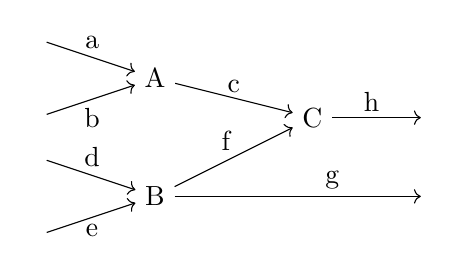
\begin{tikzpicture}
    [scale=.5, auto=center]
    \node (a) at (0,5) {};
    \node (b) at (0,3) {};
    \node (d) at (0,2) {};
    \node (e) at (0,0) {};
    \node (h) at (10,3) {};
    \node (A) at (3,4) {A};
    \node (B) at (3,1) {B};
    \node (C) at (7,3) {C};
    \node (g) at (10,1) {};
    \node (a_1) at (1.4,4.9) {a};
    \node (b_1) at (1.4,3) {b};
    \node (d_1) at (1.4,2) {d};
    \node (e_1) at (1.4,0.14) {e};
    \node (c_1) at (5,3.8) {c};
    \node (f_1) at (4.8,2.4) {f};
    \node (g_1) at (7.5,1.4) {g};
    \node (h_1) at (8.5,3.4) {h};
    \draw[->]
        (a) edge (A) (b) edge (A) (d) edge (B) (e) edge (B) (A) edge (C) (C) edge (h) (B) edge (g) (B) edge (C); 
\end{tikzpicture}
\end{center}
where the "inputs" at each node are covectors and the "outputs" are vectors. Therefore, the entire diagram, which represents the tensor $X$ has a total of 4 inputs (indices $a, b, d, e$) and two outputs (indices $h, g$). We can see from the diagram that the indices $c$ and $f$, which travels "between" the factors are the ones that are being contracted. Therefore, the contraction of $c$ and $f$ contracts the rank (4,6) tensor $A \otimes B \otimes C$ to a rank (2,4) tensor. 
\end{definition}

\begin{definition}
The \textit{tensor algebra} of vector space $V$ over field $\mathbb{F}$ is an associative, noncommutative algebra defined
\begin{align*}
    T(V) \equiv \bigoplus_{n = 0}^{\infty} V^{\otimes n} & = V^{\otimes 0} \oplus V^{\otimes 1} \oplus V^{\otimes 2} \oplus V^{\otimes 3} \oplus ... \\
    & = \mathbb{F} \oplus V \oplus V^{\otimes 2} \oplus V^{\otimes 3} \oplus V^{\otimes 4} \oplus ...
\end{align*}
with elements being infinite-tuples
\[ (a, B^\mu, C^{\nu \gamma}, D^{\alpha \beta \epsilon}, ...)\]
The addition operation is defined component-wise, and the multiplication operation is the tensor product 
\[\otimes: T(V) \times T(V) \longrightarrow T(V)\]
and the identity element is
\[I = (1, 0, 0, ...) \]
Linearity is easily proved. 
\end{definition}

The tensor algebra is used to "add" differently ranked tensors together. In order to do this rigorously, we must define the map (which is also an isomorphism)
\[i_j: V^{\otimes j} \longrightarrow T(V), \; i_j (T^{\kappa_1, ..., \kappa j}) = (0, ...,0, T^{\kappa_1, ..., \kappa j}, 0, ..., 0) \]
So, we can implicitly define the addition of arbitrary tensors $A \in V^{\otimes n}$ and $B \in V^{\otimes m}$ as 
\[ A + B \equiv i_n (A) + i_m (B) \in T(V)\]
along with the tensor multiplication of the form
\[ A \otimes B \equiv i_n(A) \otimes i_m(B) \equiv i_{n+m} (A \otimes B)\]
This allows us to alternatively define the tensor product operation as
\[i_i(V^{\otimes i}) \otimes i_j( V^{\otimes j}) \equiv i_{i+j} (V^{\otimes (i+j)})\]

\subsection{Exterior Algebras and Symmetric Algebras}
We can define the symmetric and exterior algebras multiple ways. In here, we will construct their powers separately as quotient spaces and direct sum them to create their respective algebras. But first, we must introduce the Schmidt decomposition, which is the foundation of all the results of this section. 

\begin{theorem}[Schmidt Decomposition]
For any $w \in U \otimes V$, where $U, V$ ($\dim{U} = n, \dim{V} = m$)  are inner product spaces over $\mathbb{F} \in \{ \mathbb{R}, \mathbb{C}\}$, there exists an orthonormal basis $\{u_i\}$ of $U$ and $\{v_j\}$ of $V$ such that 
\[ w = \sum_{i=1}^{\min{\{n, m\}}} \alpha_i u_i \otimes v_i, \; \alpha_i \in \mathbb{F}\]
\end{theorem}
\begin{proof}
Since $U \otimes V \simeq $ Hom$(V^*, U)$, we can interpret $w$ as a matrix $\Tilde{w}$. Using singular value decomposition, there exists unitary matrices $A, B$ and diagonal matrix $\Sigma$ such that
\[\Tilde{w} = A \Sigma B^\dagger\]
$C(A)$ and $R(B^\dagger)$ determine the orthonormal basis of $U \otimes V$, and we can thus see that the minimum number of required $u \otimes v$'s is precisely the number of nonzero singular values, which is the rank of $\Tilde{w}$. 

\end{proof}

\begin{definition}
Let $I$ be a subspace of $V \otimes V$ generated by elements of the form $x \otimes x \in V \otimes V$. That is, given a basis $\{e_i\}$ of $n$-dimensional space $V$, all tensors of the form $x \otimes x \in V \otimes V$ can be written 
\[x \otimes x = \sum_{i=1}^n a_i (e_i \otimes e_i) + \sum_{i \neq j} b_{i j} (e_i \otimes e_j + e_j \otimes e_i)\]
which implies that the components of $e_i \otimes e_j$ and $e_j \otimes e_i$ must be the same for every element in $I$. 
\end{definition}

\begin{example}
Given that $V$ is 2-dimensional, a vector $x \in V$ can be written $x = a e_1 + b e_2$, which implies
\begin{align*}
    x \otimes x & = (a e_1 + b e_2) \otimes (a e_1 + b e_2) \\
    & = a^2 (e_1 \otimes e_1) + a b (e_1 \otimes e_2) + b a (e_2 \otimes e_1) + b^2 (e_2 \otimes e_2) \\
    & = a^2 (e_1 \otimes e_1) + b^2 (e_2 \otimes e_2) + a b (e_1 \otimes e_2 + e_2 \otimes e_1) 
\end{align*}
\end{example}

Since we can group the components $e_i \otimes e_j$ and $e_j \otimes e_i$ together to $e_i \otimes e_j + e_j \otimes e_i$, the basis of $I$ is 
\[\{e_1 \otimes e_1, ..., e_n \otimes e_n, e_1 \otimes e_2 + e_2 \otimes e_1, ..., e_{n-1} \otimes e_n + e_n \otimes e_{n-1}\}\]

\begin{definition}
Now, we can define the \textit{second exterior power of $V$} as
\[\Lambda^2 V \equiv \frac{V \otimes V}{I}\]
and it follows that 
\[\dim{\Lambda^2 V} = n^2 - \dim{I} = \frac{1}{2} n (n-1)\]
We denote the elements of $\Lambda^2 V$ as $x \wedge y$, which really just represents the equivalence class of $x \otimes y$ in the quotient space. It is clear that $x \otimes x \in I \implies x \wedge x = 0$, so
\begin{align*}
    0 = (x + y) \wedge (x + y) & = x \wedge x + x \wedge y + y \wedge x + y \wedge y \\
    & = x \wedge y + y \wedge x \\
    \implies & x \wedge y = - y \wedge x
\end{align*}
That is, the wedge product is antisymmetric. Note also that we can assume distributivity of $\wedge$ since it is just the quotient operation of another operation $\otimes$ that satisfies distributivity. 
\\

We can construct a basis on $\Lambda^2 V$, given by 
\[\{e_i \wedge e_j \; | \; i < j\}\]
Again, we note that $i < j$ since $e_i \wedge e_i = 0$ and $e_i \wedge e_j = - e_j \wedge e_i$. 
\end{definition}

One realization of the space $\Lambda^2 \mathbb{R}^n$ is the set of antisymmetric $n \times n$ matrices. 
\\

We can construct higher order exterior powers, too. For $n = 3$ (and assuming that $\dim{V} \geq 3$), the subspace $I \subset V \otimes V \otimes V$ is the space generated by elements of the forms
\[x \otimes x \otimes y, x \otimes y \otimes x, y \otimes x \otimes x\]
Following a similar construction, the \textit{third exterior power of $V$} is
\[\Lambda^3 V \equiv \frac{V \otimes V \otimes V}{I}\]
with its elements being equivalence classes of the form
\[x \wedge y \wedge z,\; x, y, z \in V\]
such that
\begin{align*}
    x \wedge y \wedge z & = - x \wedge z \wedge y \\
    & = - y \wedge x \wedge z \\
    & = - z \wedge y \wedge x
\end{align*}
The basis of $\Lambda^3 V$ is
\[\{e_i \wedge e_j \wedge e_k \; | \; i < j < k\} \implies \dim{\Lambda^3 V} = \frac{1}{6} n (n-1) (n-2)\]
Generally, if $\sigma$ is a permutation of the ordered list $(1, 2, ..., n)$, and $x_1, x_2, ..., x_n \in V$, then 
\[x_{\sigma(1)} \wedge x_{\sigma(2)} \wedge ... \wedge_{\sigma(n)} = sgn(\sigma) \; x_1 \wedge x_2 \wedge ... \wedge x_n\]
which means that if $x_i = x_j$ for some $1 \leq i \neq j \leq n$, 
\[x_1 \wedge x_2 \wedge ... \wedge x_n = 0\]
By constructing all the exterior powers of $n$-dimensional space $V$, we can construct the algebra 
\begin{align*}
    \Lambda(V) \equiv \bigoplus_{k=0}^n \Lambda^k V \equiv \Lambda^0 V \oplus \Lambda^1 V \oplus \Lambda^2 V \oplus ... \oplus \Lambda^n V 
\end{align*}
Note that $\Lambda^0 V = \mathbb{F}$ and $\Lambda^1 V = V$. Unlike the tensor algebra, the exterior algebra is finite since the exterior powers vanish for finite $n$. In fact, 
\[ \dim{\Lambda^k V} = \begin{cases}
_n C_k & 0 \leq k \leq n \\
0 & n < k
\end{cases}\]
which implies that 
\[\dim{\Lambda(V)} = 2^n \]
\begin{definition}
The $n$th exterior power $\Lambda^n V$ is 1 dimensional, spanned by the singular basis vector 
\[e_1 \wedge e_2 \wedge ... \wedge e_{n-1} \wedge e_n\]
This vector is the \textit{determinant}. Note that this construction of the determinant is consistent with our previous construction of the determinant of a matrix since $e_1 \wedge ... \wedge e_n$ is indeed multilinear and antisymmetric. In its purest sense, 
\[e_1 \wedge ... \wedge e_n: \prod_{i=1}^n V^* \longrightarrow \mathbb{F}\]
is a mapping that is multilinear and antisymmetric. But there is an inconsistency. The matrix determinant takes in \textit{matrices} rather than taking in $n$-tuples of covectors. However, we can interpret the $n$ covectors in $V^* \times ... \times V^*$ as the column (or row) vectors of an $n \times n$ matrix. This completes the realization, and so we can conclude that the matrix determinant is just a realization of the more abstract determinant $e_1 \wedge ... \wedge e_n$. 

Note that any tensor in $\Lambda^n V$ satisfies multilinearity and antisymmetricity, but only the basis vector $e_1 \wedge ... \wedge e_n$ satisfies the normalizing condition
\[\det{I} = 1\]
Since, given that the dual basis of $V^*$ is $\{f_j\}$
\[(e_1 \wedge ... \wedge e_n) (f_1, f_2, ..., f_n) = \prod_{i=1}^n e_i (f_i) = \prod_{i=1}^n \delta_i^i = 1\]
\end{definition}

\begin{example}
Given 3 dimensional vector space $V$ with basis $\{e_1, e_2, e_3\}$, the wedge product of two vectors $a, b \in V$ is 
\begin{align*}
    a \wedge b & = (a_1 e_1 + a_2 e_2 + a_3 e_3) \wedge (b_1 e_1 + b_2 e_2 + b_3 e_3) \\
    & = (a_2 b_3 - a_3 b_2) e_2 \wedge e_3 + (a_3 b_1 - a_1 b_3) e_3 \wedge e_1 + (a_1 b_2 - a_2 b_1) e_1 \wedge e_2 
\end{align*}
which is essentially the formula for the cross product $\times$ in Euclidean space. We can therefore think of the realization of the wedge product in 3 dimensional space $V$ as the cross product. 
\[\wedge: V \times V \longrightarrow \Lambda^2 V\]
Note that $\Lambda^2 V \simeq V$ if $\dim{V} = 3$, so we can construct the more familiar $\times$ operation in $\mathbb{R}^3$. 
\[\times: \mathbb{R}^3 \times \mathbb{R}^3 \longrightarrow \Lambda^2 \mathbb{R}^3 \simeq \mathbb{R}^3\]
which is consistent with $\times$ taking two vectors and outputting a third vector living in $\mathbb{R}^3$ that is orthogonal to the two input vectors. 
\end{example}

\begin{example}
The realization of the wedge product of 3 vectors in 3 dimensional space $V$ is the \textit{triple scalar product}, which we will denote as $\times_3$
\[\wedge: V \times V \times V \longrightarrow \Lambda^3 V\]
Note that since $\Lambda^3 V \simeq V$ when $\dim{V} = 3$, we can write 
\[\times_3: \mathbb{R}^3 \times \mathbb{R}^3 \times \mathbb{R}^3 \longrightarrow \Lambda^3 \mathbb{R}^3 \simeq \mathbb{R}\]
which is consistent with $\times_3$ taking three vectors and outputting the signed volume of their parallelopiped which lies in $\mathbb{R}$. 
\end{example}

Now we introduce the symmetric algebra and its construction. Let $I$ be the subspace of $V \otimes V$ generated by all tensors of the form 
\[u \otimes v - v \otimes u, \; u, v \in V\]
For example, given $a, b \in V$ with basis $\{e_1, e_2\}$, 
\begin{align*}
    a \otimes b - b \otimes a & = (a_1 e_1 + a_2 e_2) \otimes (b_1 e_1 + b_2 e_2) - (b_1 e_1 + b_2 e_2) \otimes (a_1 e_1 + a_2 e_2) \\
    & = (a_1 b_2 - b_2 a_1) e_1 \otimes e_2 + (a_2 b_1 - b_2 a_1) e_2 \otimes e_1 
\end{align*}
is an element of $I$. We can generalize this to see that
\[\{e_i \otimes e_j - e_j \otimes e_i\}, \; i \neq j\]
is the basis for $I$. Now, let us define the \textit{second symmetric power of $V$} as 
\[\Sym^2 V \equiv \frac{V \otimes V}{I}\]
where, given that $\dim{V} = n$, 
\[\dim{\Sym^2 V} = n^2 - \frac{1}{2} n (n-1) = \frac{1}{2} n (n+1)\]
We denote the elements of $\Sym^2 V$ as $x \odot y$, which are really the equivalence classes $\{x \otimes y - y \otimes x\}$. Note that
\begin{align*}
    x \odot y - y \odot x & = \{x \otimes y - y \otimes x\} - \{ y \otimes x - x \otimes y\} \\
    & = \{ x \otimes y - y \otimes x - y \otimes x + x \otimes y\} \\
    & = \{0\} = 0
\end{align*}
$\implies x \odot y = y \odot x$. That is, the $\odot$ operator is symmetric, and $\Sym^2 V$ has basis 
\[ \{e_i \odot e_j\}_{j \geq k}\]
One realization of $\Sym^2 \mathbb{R}^n$ is the set of all symmetric $n \times n$ real matrices. 
\\

We can construct higher symmetric powers satisfying this property that its tensors are invariant under transpositions. 
\[x_1 \odot ... x_i \odot ... x_j \odot ... x_n = x_1 \odot ... x_j \odot ... x_i \odot ... x_n\]
for all $1 \leq i \neq j \leq n$, which implies that it is invariant under any permutation $p \in S_n$ of the $x_i$'s. Additionally, 
\[\dim{\Sym^k V} = {{n+k-1} \choose k }\]

\begin{definition}
The \textit{symmetric algebra} of vector space $V$ is constructed as such 
\[\Sym (V) \equiv \bigoplus_{k=0}^\infty \Sym^k V\]
Note that unlike the exterior algebra, $\Sym(V)$ is infinite dimensional. 
\end{definition}

\begin{example}
The inner product $(\cdot, \cdot)$ on $V$ is an element of $\Sym^2 V$, since it is a bilinear, symmetric operation on $V$. 
\[\odot, (\cdot, \cdot): V \times V \longrightarrow \mathbb{F}\]
\end{example}

There is a simple relationship between $V \otimes V$, $\Lambda^2 V$, and $\Sym^2 V$. 

\begin{theorem}
\[V \otimes V \simeq \Sym^2 V \oplus \Lambda^2 V\]
with isomorphism defined
\[v \otimes w \mapsto \Big( \frac{1}{2} (v \odot w), \frac{1}{2} (v \wedge w) \Big)\]
This is precisely the factoring of a rank (2,0) tensor into its symmetric and antisymmetric parts. 
\end{theorem}
\begin{proof}
Given $v \otimes w \in V \otimes V$, 
\[v \otimes w + w \otimes v \in \Sym^2 V \text{ and } v \otimes w - w \otimes v \in \Lambda^2 V\]
By defining $v \odot w$ and $v \wedge w$ as the expressions above, the isomorphism is satisfied. 
\end{proof}

Therefore, when working in $V \otimes V$, we can interpret 
\begin{align*}
    & v \wedge w = \frac{1}{2} (v \otimes w - w \otimes v) \\
    & v \odot w = \frac{1}{2} (v \otimes w + w \otimes v) 
\end{align*}

However, 
\[V \otimes V \otimes V \not\simeq \Sym^3 V \oplus \Lambda^3 V\]
\textit{Schur functors} are used to fix this discrepancy. 

Note that we have introduced these two algebras by first constructing the quotient spaces $\Lambda^n V$ and $\Sym ^n V$ from the tensor product spaces $T^{\otimes n}$ and then direct summing these powers to construct the algebras. We will introduce another type of construction that directly takes the quotient algebra of $T(V)$ with the two-sided ideal. 



\end{document}
